\documentclass[12pt]{report}
\usepackage{bm,amsmath,amsthm,amssymb,graphicx,listings,hyperref}
\usepackage{fullpage}
\usepackage{ccicons,xmpincl}
\usepackage[usenames,dvipsnames]{color}
\usepackage{mcode}
\newtheorem{theorem}{Theorem}[section]
\newtheorem{lemma}{Lemma}[section]
\newtheorem{corollary}{Corollary}[section]
\newtheorem{definition}{Definition}[section]
\newtheorem{proposition}{Proposition}[section]
\newtheorem{conjecture}{Conjecture}[section]
\newtheorem{remark}{Remark}[section]
\newtheorem{example}{Example}[section]

%% \setlength{\hoffset}{0cm}
%% \setlength{\marginparwidth}{0cm}
%% \setlength{\textwidth}{6.5in}

\definecolor{lightpurple}{rgb}{0.8,0.8,1}
\definecolor{gray}{rgb}{0.8,0.8,0.8}

\lstset{
  showstringspaces=false,
  numbers=left,
  stepnumber=1,
  numbersep=5pt,
  numberstyle=\tiny\color{black},
  showtabs=false,
  tabsize=2,
  captionpos=t,
  basicstyle=\footnotesize\ttfamily,
  breaklines=true,
  backgroundcolor=\color{white},
  frame=lines,
  rulesepcolor=\color{gray}
}

\lstdefinestyle{matlab_style}{
  %% backgroundcolor=\color{gray}
}

\lstdefinestyle{fortran_style}{
  %% backgroundcolor=\color{gray}
}

\lstdefinestyle{make_style}{
  backgroundcolor=\color{gray}
}

\lstdefinestyle{bash_style}{
  backgroundcolor=\color{gray}
}

\lstdefinestyle{python_style}{
  %% backgroundcolor=\color{gray}
}

\title{Parallel Spectral Numerical Methods}
\author{Gong Chen, Brandon Cloutier, Ning Li, Benson K. Muite and Paul Rigge \\ with contributions from\\ Sudarshan Balakrishnan, Andre Souza and Jeremy West}
\begin{document}
\maketitle

\tableofcontents

\newpage
\phantomsection \label{listoffig}
\addcontentsline{toc}{chapter}{List of Figures}
\listoffigures

\newpage
\phantomsection \label{listoflistings}
\addcontentsline{toc}{chapter}{Program Listings}
\lstlistoflistings

\chapter*{License}
This work is licensed under the Creative Commons Attribution 3.0 Unported
License. To view a copy of this license, visit
\url{http://creativecommons.org/licenses/by/3.0/} or send a letter to Creative
Commons, 444 Castro Street, Suite 900, Mountain View, California, 94041, USA.

The programs are available under the simplified BSD license:

Copyright \copyright 2012, Gong Chen, Brandon Cloutier, Ning Li , Benson Muite, Paul Rigge and Sudarshan Balakrishnan, Andre Souza Jeremy West. All rights reserved.

Redistribution and use in source and binary forms, with or without modification, are permitted provided that the following conditions are met:

    Redistributions of source code must retain the above copyright notice, this list of conditions and the following disclaimer.
    Redistributions in binary form must reproduce the above copyright notice, this list of conditions and the following disclaimer in the documentation and/or other materials provided with the distribution.

THIS SOFTWARE IS PROVIDED BY THE COPYRIGHT HOLDERS AND CONTRIBUTORS "AS IS" AND ANY EXPRESS OR IMPLIED WARRANTIES, INCLUDING, BUT NOT LIMITED TO, THE IMPLIED WARRANTIES OF MERCHANTABILITY AND FITNESS FOR A PARTICULAR PURPOSE ARE DISCLAIMED. IN NO EVENT SHALL THE COPYRIGHT HOLDER OR CONTRIBUTORS BE LIABLE FOR ANY DIRECT, INDIRECT, INCIDENTAL, SPECIAL, EXEMPLARY, OR CONSEQUENTIAL DAMAGES (INCLUDING, BUT NOT LIMITED TO, PROCUREMENT OF SUBSTITUTE GOODS OR SERVICES; LOSS OF USE, DATA, OR PROFITS; OR BUSINESS INTERRUPTION) HOWEVER CAUSED AND ON ANY THEORY OF LIABILITY, WHETHER IN CONTRACT, STRICT LIABILITY, OR TORT (INCLUDING NEGLIGENCE OR OTHERWISE) ARISING IN ANY WAY OUT OF THE USE OF THIS SOFTWARE, EVEN IF ADVISED OF THE POSSIBILITY OF SUCH DAMAGE.
\chapter*{Acknowledgements}

The example programs have used a similar structure to those in Trefethen~\cite{Tre00}, to which the reader is referred to for further code examples. The codes for the nonlinear Schr\"{o}dinger equation were developed in collaboration with Christian Klein and Kristelle Roidot. The codes for the Navier-Stokes equation were developed in collaboration with Hans Johnston. We thank Peter Miller, Brock Palen, David O'Neal,  Divakar Viswanath and Jared Whitehead for helpful comments, discussions and suggestions. A class project by Sou-Chi Chang and Sophie Zhang, influenced the presentation of the nonlinear Schr\"{o}dinger equation and the exercises on the Gross-Pitaevskii equation, while a class project by Fuzhou Hu and Yutao Qin influenced the presentation and exercises for the two dimensional Navier-Stokes equations. We also thank Daniel Brahan, Emily Cizmas, Kohei Harada, Seth Jordan, Joshua Kirschenheiter, Brian Leu, Albert Liu, Thomas Olsen, Henry Rensch, Parth Sheth, Jeffrey Smolik and Matthew Warnez for constructive criticism and testing the materials. We thank Danny Ellis for providing his notes taken during a lecture on some of this material. 

This tutorial was produced using resources of:
\begin{itemize}
\item  Hopper at the National Energy Research Scientific Computing Center, which is supported by the Office of Science of the U.S. Department of Energy under Contract No. DE-AC02-05CH11231. 
\item The Extreme Science and Engineering Discovery Environment (XSEDE), which is supported by National Science Foundation grant number OCI-1053575.
\item Jaguar at the Oak Ridge Leadership Computing Facility at the Oak Ridge National Laboratory, which is supported by the Office of Science of the U.S. Department of Energy under Contract No. DE-AC05-00OR22725.
\item SCREMS NSF DMS-1026317
\end{itemize}

Partial financial support was also provided by:
\begin{itemize}
\item A curriculum material development grant from The Blue Waters Undergraduate Petascale Education Program  administered by the Shodor foundation.
\item A Faculty Grant for Innovations in Teaching with Technology from the division of Literature, Sciences and Arts at the  University of Michigan.
\item CNRS (Centre National de la Recherche Scientifique)
\end{itemize}

This tutorial utilizes the following packages:
\begin{itemize}
\item Mcode created by Florian Knorn which can be downloaded at \url{http://www.mathworks.com/matlabcentral/fileexchange/8015-m-code-latex-package}
\end{itemize}
\chapter{Overview}
\section{Summary}
We start by taking a quick look at finite-precision arithmetic. We then discuss how to solve ordinary differential equations (ODE) and partial differential equations (PDE) using the technique of separation of variables. We then introduce numerical time-stepping schemes that can be used to solve ODEs and PDEs. Next we introduce pseudo spectral methods by giving an overview of the discrete Fourier Transform (DFT) and the Fast Fourier Transform (FFT) algorithm that is used to quickly calculate the DFT. Finally we will combine all of this to solve a couple of different PDEs first in a serial setting and then in a parallel setting. The programs will use Matlab\footnote{\url{http://www.mathworks.com/products/matlab/index.html} -- if this is not available, we suggest modifying the Matlab programs to use Octave which can be freely downloaded at {\url{http://www.gnu.org/software/octave/}}.} and Fortran. A Python{\footnote{\url{http://python.org/}} implementation of some of the Matlab programs is also provided. 

\section{Prerequisites}
We assume that the reader has introductory programming experience, for example using C, C++, Fortran, Matlab, Octave, Python or equivalent. Since detailed programming examples have been provided, we do not expect a significant programming background, but hope the required knowledge will be acquired as one works through the examples. We also assume the level of mathematical maturity obtained in a demanding calculus course, for example at the level of Courant and Johns ``Introduction to Calculus and Analysis''. A course in differential equations would also be helpful, but for many scientists or engineers, their fields of interest will provide numerous examples of these. More programming experience or mathematical background will make the material easier to understand. Checking whether the simulations are correct may also be easier for those with knowledge of the behavior of solutions of the partial differential equations that are being approximated, however we have tried to choose representative differential equations that will make it easy for one to use the programs and then adapt them to the use being considered.  

\section{Using the Programs}

The programs have been tested on several different computers. The programs are located in program directories which correspond to the chapter in which the programs first appear. While they are not explicitly hyperlinked, one can find their locations either by reading the LaTeX source code or by searching the appropriate directory.

The Matlab programs are guaranteed to work with Matlab R2011b, but should also work with other recent versions of Matlab. They should also be easy to modify so that they work with Octave. The Fortran programs have been tested primarily with the GCC 4.6.2 compiler suite, although they should work with most other recent compilers. If using an implementation of MPI that depends on a particular compiler, we suggest also using the GCC compiler. We expect that the programs should work with minor modifications with other compilers, but cannot guarantee this.  For simplicity and to allow checking of program correctness, we have chosen to use a low compiler optimization level. We encourage users to increase the compiler optimization level and compiler flags once they have checked that the programs are working correctly on their systems. FFTW, a free Fast Fourier transform library, is also required to run the programs. This can be downloaded from \url{http://fftw.org/}. The MPI programs make use of the library 2DECOMP\&FFT which can be downloaded from \url{http://www.2decomp.org}. Finally, the last part of the tutorial requires the use of the free and open source VisIt parallel visualization program, which can be obtained from \url{https://wci.llnl.gov/codes/visit/home.html}. If you expect to do large parallel simulations (A guide for large at present is 20\% of the system for systems larger than 10,000 cores), it may be worth learning the most efficient system settings for performing output and for parallelization. We do not address this in this tutorial, but suggest that you contact your computing center for suggestions.

\section{Course Outlines / Assessment Rubric}

The material in these notes can form the basis of a short course. The most important portions are chapters 1 to  11.  A selection can then be made from chapters 12, 13 and 14. A selection of the problems can be used to assess student learning. Note that problems in chapters 8.  12, 13 and 14 can develop into extensive research projects, so only a sample of these should be given to any students if they only have a limited time to solve them. A student will have successfully understood the material if they can run the example Matlab/Python, serial Fortran, OpenMP Fortran and MPI Fortran programs, and can also modify them to solve related problems. Successful completion of problems which test these abilities will be enough to indicate that students have understood the fundamental concepts.
\chapter{Finite Precision Arithmetic}

\footnote{For more on this see a text book on numerical methods such as Bradie~\cite{Bra06}.} Because computers have a fixed amount of memory, floating point numbers can only be stored with a finite number of digits of precision. This limits the accuracy to which the solution to a numerical problem can be obtained in finite time. Most computers use binary IEEE 754 arithmetic to perform numerical calculations. There are other formats, but this will be the one of most relevance to us.

%subsubsection
\section{Exercises}
\begin{enumerate}
\item[1)] Download the most recent IEEE 754 standard. \url{http://ieeexplore.ieee.org/xpl/mostRecentIssue.jsp?punumber=2355}, see also \url{http://grouper.ieee.org/groups/754/} -- unfortunately the links to the official standard requires either IEEE membership or a subscription. If you do not have this please see the wikipedia page (\url{http://en.wikipedia.org/wiki/IEEE_754-2008}) for the information you will need to answer the questions below\footnote{These links are correct as of 1 April 2012, should they not be active, we expect that the information should be obtained by a search engine or by referring to a numerical analysis textbook such as Bradie~\cite{Bra06}.}.
\begin{enumerate}
\item[a)] In this standard what is the range and precision of numbers in:
\begin{enumerate}
\item[i)] Single precision
\item[ii)] Double precision
\end{enumerate} 
\item[b)] What does the standard specify for quadruple precision?
\item[c)] What does the standard specify about how elementary functions should be computed? How does this affect the portability of programs?
\end{enumerate}
\item[2)] Suppose we discretize a function for $x\in[-1,1]$. For what values of $\epsilon$ is
$$\epsilon\log\left(\cosh\left(\frac{x}{\epsilon}\right)\right)=\lvert x \rvert$$
in
\begin{enumerate}
\item[i)] Single precision?
\item[ii)] Double precision?
\end{enumerate} 
\item[3)] Suppose we discretize a function for $x\in[-1,1]$. For what values of $\epsilon$ is
\begin{align*}
&{}\tanh\left(\frac{x}{\epsilon}\right)
=\left\{{1 \quad x\geq0}\atop{-1 \quad x < 0}\right.
\end{align*}
in
\begin{enumerate}
\item[i)] Single precision?
\item[ii)] Double precision?
\end{enumerate} 
\item[4)] 
\begin{enumerate}
\item[a)] What is the magnitude of the largest  4 byte integer in  the IEEE 754  specification that can be stored?
\item[b)] Suppose you are doing a simulation with $N^3$ grid points and need to calculate $N^3$. If $N$ is stored as a 4 byte integer, what is the largest value of $N$ for which $N^3$ can also be stored as a 4 byte integer?
\end{enumerate}
\end{enumerate}

\chapter{Separation of Variables}
Separation of variables is a technique which can be used to solve both ODEs and PDEs. The basic idea for an equation in two variables is to rewrite the equation so that each of the two variables is located on different sides of an equality sign, and since both sides of the equation depend on different variables, the two sides must be equal to a constant. We introduce this idea with the simple first order linear ODE
\begin{eqnarray}\label{eq:simpleode}
\ \frac{dy}{dt}=y.
\end{eqnarray}
As long as $y(t) \neq 0$ for any value of $t$, we can formally separate variables and rewrite eq.\ \eqref{eq:simpleode} as
\begin{eqnarray}
\ \frac{dy}{y}=dt.
\end{eqnarray}
Now we can solve for $y(t)$ by integrating both sides
\begin{eqnarray}
\int{\frac{dy}{y}}&=&\int{dt} \\
\ln{y}+a&=&t+b \\
e^{\ln{y}+a}&=&e^{t+b} \\
e^{\ln{y}}e^{a}&=&e^te^b \\
y&=&\frac{e^b}{e^a} e^t \\
y(t)&=&c e^t.
\end{eqnarray}
Where $a$, $b$, and $c$ are arbitrary constants of integration. 

We now perform a similar example for a linear partial differential equation. The heat equation is 
\begin{equation}
u_t=-u_{xx}.
\end{equation}
We suppose that $u=X(x)T(t)$, so that we obtain
\begin{equation}
X(x)\frac{\mathrm{d}T}{\mathrm{d}t}(t)=-\frac{\mathrm{d}^2X}{\mathrm{d}x^2}(x)T(t).
\end{equation}
We can rewrite this as
\begin{equation}
\frac{\frac{\mathrm{d}T}{\mathrm{d}t}(t)}{T(t)}=\frac{\frac{\mathrm{d}^2X}{\mathrm{d}x^2}(x)}{X(x)}=-C,
\end{equation}
where $C$ is a constant independent of $x$ and $t$. The two sides can be integrated separately to get $T(t)=\exp(-Ct)$ and either $X(x)=\sin(\sqrt{C}x)$ or $X(x)=\cos(\sqrt{C}x)$. Since the heat equation is linear, one can then add different solutions to the heat equation and still obtain a solution of the heat equation. Hence solutions of the heat equation can be found by
\begin{equation}
\sum_n \alpha_n\exp(-C_nt)\sin(\sqrt{C_n}x) + \beta_n\exp(-C_nt)\cos(\sqrt{C_n}x)
\end{equation}
where the constants $\alpha_n$, $\beta_n$ and $C_n$ are appropriately chosen. Convergence of such series to an actual solution is studied in mathematics courses on analysis (see for example Evans~\cite{Eva10} or Renardy and Rogers~\cite{RenRog04}), however the main ideas necessary to choose the constants, $\alpha_n$, $\beta_n$ and $C_n$ and hence construct such solutions are typically encountered towards the end of a calculus course or at the beginning of a differential equations course, see for example Courant and John~\cite{CouJoh98} or Boyce and DiPrima~\cite{BoyDip10}. Here, we consider the case where $x\in[0,2\pi]$, and for which we have periodic boundary conditions. In this case $\sqrt{C_n}$ must be integers, which we choose to be non-negative to avoid redundancies. At time $t=0$, we shall suppose that the initial condition is given by 
\begin{equation}
u(x,t=0)=f(x).
\end{equation}
Now, 
\begin{align}
&{} \int_0^{2\pi}\sin(nx)\sin(mx)=\left\{{\pi\quad m=n}\atop{0 \quad m\ne n}\right.,
\\&{} \int_0^{2\pi}\cos(nx)\cos(mx)=\left\{{\pi\quad m=n}\atop{0 \quad m\ne n}\right.,
\end{align}
and
\begin{align}
&{} \int_0^{2\pi}\cos(nx)\sin(mx)=0.
\end{align}
Thus we can consider the trigonometric polynomials as being orthogonal vectors. It can be shown that a sum of these trigonometric polynomials can be used to approximate a wide class of periodic functions on the interval $[0,2\pi]$; for well behaved functions, only the first few terms in such a sum are required to obtain highly-accurate approximations. Thus, we can suppose that
\begin{equation}
f(x)=\sum_n  \alpha_n\sin(\sqrt{C_n}x) + \beta_n\cos(\sqrt{C_n}x).
\end{equation}
Multiplying the above equation by either $\sin(\sqrt{C_n}x)$ or $\cos(\sqrt{C_n}x)$ and using the orthogonality of the functions, we deduce that
\begin{equation}
\alpha_n=\frac{\int_0^{2\pi}f(x)\sin(\sqrt{C_n}x)\mathrm{d}x}{\int_0^{2\pi}\sin^2(\sqrt{C_n}x)\mathrm{d}x}
\end{equation}
and
\begin{equation}
\beta_n=\frac{\int_0^{2\pi}f(x)\cos(\sqrt{C_n}x)\mathrm{d}x}{\int_0^{2\pi}\cos^2(\sqrt{C_n}x)\mathrm{d}x}.
\end{equation}

Most ODEs and PDEs of practical interest will not be separable. However, the ideas behind separation of variables can be used to allow one to find series solutions to a wide class of PDEs. These series solutions can also be found numerically and are what we will use to find approximate solutions to PDEs, and so the ideas behind this simple examples are quite useful.

%%%%%%%
%  Section
%%%%%%%
\section{Exercises}
\begin{enumerate}
\item[1)] Solve the ordinary differential equation
$$u_t=u(u-1)\quad u(t=0)=0.8$$
using separation of variables.
\item[2)] 
\begin{enumerate}
\item[a)] Use separation of variables to solve the partial differential equation 
$$u_{tt}=u_{xx}$$
with
$$u(x=0,t)=u(x=2\pi,t),$$
$$u(x,t=0)=\sin(6x)+\cos(4x)$$
and
$$u_t(x,t=0)=0.$$
\item[b)] Create plots of your solution at several different times and/or create an animation of the solution you have found.\footnote{Your solution should involve only a few modes and so you should be able to use a wide variety of software to create plots, for example a graphing calculator, a spreadsheet program such as Excel, Mathematica, Wolfram Alpha, Matlab, Maple, Python, Sage etc. You can use Wolfram Alpha and Sage online.} 
\item[c)]  The procedure required to find the coefficients in the Fourier series expansion for the initial condition can become quite tedious/intractable. Consider the initial condition $u(x,t=0)=\exp(\sin(x))$. Explain why it would be difficult to compute the Fourier coefficients for this by hand. Also explain why it would be nice to have an algorithm or computer program that does this for you.
\end{enumerate}
\end{enumerate}

\chapter{Motivation for Numerical Methods}
Many partial differential equations do not have exact closed-form solutions for all choices of initial conditions\footnote{An example is the Navier-Stokes equation which is thought to describe the motion of an incompressible viscous fluid.}. Irregular boundary conditions can also make finding an analytic solution difficult for many partial differentail equation. In these cases, finding an approximate solution with a numerical method can be helpful either for physical purposes, engineering purposes or for mathematical investigations of the behavior of solutions to these partial differential equations.
There are also cases where the partial differential equations have explicitly known exact solutions, but the formulae used to express the exact solutions require a large number of computations to evaluate them\footnote{An example is the sine-Gordon equation.}. In this case we are interested in making numerical approximations that result in accurate and cost-efficient solutions.

Numerical methods allows us to use a computer to calculate approximate solutions to partial differential equations. The accuracy of the solution will depend on which numerical method is used and usually more accurate numerical methods tend to be more complicated than less accurate methods. We will therefore start with some simple numerical methods to familiarize ourselves with how numerical methods work.
We encourage the reader to take a full course on the numerical solution of partial differential equations as well as reading the references to find out about numerical techniques not discussed here.


\chapter{Timestepping}
We now briefly discuss how to solve initial value problems. For more on this see Bradie~\cite[Chap. 7]{Bra06}. A slightly longer but still quick introduction to these ideas can also be found in Boyce and DiPrima~\cite{BoyDip10}.
%%%%%%%
%Section
%%%%%%%
\section{Forward Euler}
In order to compute solutions to differential equations on computers efficiently, it is convenient to do our calculations at a finite number of specified points and then interpolate between these points. For many calculations it is convenient to use a grid whose points are equally distant from each other. 

For the rest of the section $h$ will be our step size, which is assumed to be constant.  When solving an ODE or PDE, the choice of $h$ isn't selected at random, but rather requires some intuition and/or theoretical analysis. We are going to start with the forward Euler method which is the most basic numerical method. Let us first denote the time at the $n$th time-step by $t^n$ and the computed solution at the $n^{th}$ time-step by $y^n$, where $y^n \equiv y(t=t^n)$. The step size $h$ in terms of $t$ is defined as $h=t^{n+1}-t^n$. Lets first start with a basic ODE with initial conditions, in which $f(t,y)$ is some arbitrary function and $y(t)$ is our solution,
\begin{eqnarray}\label{eq:ode}
\ \frac{dy}{dt} = f(t,y) \qquad y(t^0)=y^0.
\end{eqnarray}
The differential equation can be approximated by finite differences, 
\begin{eqnarray}
\frac{y^{n+1}-y^n}{h} = f(t^n,y^n).
\end{eqnarray}
Now all we have to do is solve for $y^{n+1}$ algebraically,
\begin{eqnarray}\label{eq:odeFE}
\ y^{n+1}=y^n+h f(t^n,y^n) \qquad \text{(Forward Euler/Explicit method)}
\end{eqnarray}
If we wanted to calculate $\frac{dy}{dt}$ at time $t^0$, then we could generate an approximation for the value at time $t^{n+1}$ using \eqref{eq:odeFE} by first finding $y(t^0)$ and using it to compute $y^{n+1}$. We then repeat this process until the final time is reached.

%Subsection
\subsection{An Example Computation}
Let us consider the ODE in eq.\ \eqref{eq:ode} with $f(t,y)=y$ and initial conditions $y(t^0)=1$ where $t^0=0$. Two numerical solutions are computed using the forward Euler method with $h=1$ and $h=.1$
\begin{figure}
\begin{center}
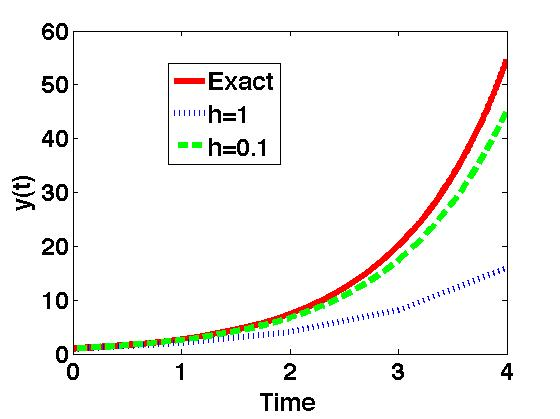
\includegraphics[scale=0.6]{./Timestepping/Forward_Euler.jpg}
\caption{A numerical solution to the ODE in eq.\ \eqref{eq:ode} with $f(t,y)=y$ demonstrating the accuracy of the Forward Euler method for different choices of timestep.} \label{fig:FEexample}
\end{center}
\end{figure}

It should be no surprise that a smaller step size like $h=.1$ compared to $h=1$ will be more accurate. Looking at the line for $h=1$, you can see that $y(t)$ is calculated at only 4 points then straight lines interpolate between each point. This is obviously not very accurate, but gives a rough idea of what the function looks like. The solution for $h=.1$ might require 10 times more steps to be taken, but it is clearly more accurate. Forward Euler is an example of a first-order method and approximates the exact solution using the first two terms in the Taylor expansion\footnote{The derivation of the Taylor expansion can be found in most books on calculus.}
\begin{eqnarray}
y(t^n+h)=y(t^n)+h \left.\frac{dy}{dt}\right|_{t^n}+\text{O}(h^2),
\end{eqnarray}
where terms of higher order than O$(h^2)$ are omitted in the approximate solution. Substituting this into eq.\ \eqref{eq:odeFE} we get that
\begin{align*}
&{} y^n +h \left.\frac{dy}{dt}\right|_{t^n}+\text{O}(h^2) = y^n +hf(t^n,y^n)
\end{align*}
after cancelling terms and dividing by $h$, we get that
\begin{align*}
&{} \left.\frac{dy}{dt}\right|_{t^n}+\text{O}(h) = f(t^n,y^n),
\end{align*}
from which it is clear that the accuracy of the method changes linearly with the step size, and hence it is first-order accurate.
%%%%%%%
%Section
%%%%%%%
\section{Backwards Euler}
A variation of forward Euler can be obtained by approximating a derivative by using a backward difference quotient. Using eq.\ \eqref{eq:ode} and applying
\begin{eqnarray}
\frac{y^{n}-y^{n-1}}{h}&\approx&f(t^n,y^n) \\
y^{n}&=&y^{n-1}+h f(t^n,y^n).
\end{eqnarray}
Stepping the index up from $n$ to $n+1$ we obtain,
\begin{eqnarray}
y^{n+1}=y^n+h f(t^{n+1},y^{n+1})\qquad \text{(Backwards Euler/Implicit method)}
\end{eqnarray}
Notice how $y^{n+1}$ is not written explicitly like it was in the forward Euler method. This equation instead implicitly defines $y^{n+1}$ and must be solved  to determine the value of $y^{n+1}$. How difficult this is depends entirely on the complexity of the function $f$. For example, if $f$ is just $y^2$, then the quadratic formula could be used, but many nonlinear PDEs require other methods. Some of these methods will be introduced later.
%%%%%%%
%Section
%%%%%%%
\section{Crank-Nicolson}
By taking an average of the forward and backward Euler methods, we can find the Crank-Nicolson method:
\begin{eqnarray}
\frac{y^{n+1}-y^{n}}{h}&=&\frac{1}{2}f(t^{n+1},y^{n+1})+\frac{1}{2}f(t^n,y^n)
\end{eqnarray}
Rearranging we obtain,
\begin{eqnarray}
y^{n+1}=y^n+\frac{h}{2}\left[ f(t^{n+1},y^{n+1})+f(t^n,y^n) \right] \qquad \text{(Crank-Nicolson)}
\end{eqnarray}
Notice again how $y^{n+1}$ is not written explicitly like it was in forward Euler. This equation instead implicitly defines $y^{n+1}$ and so the equation must be solved algebraically to obtain $y^{n+1}$. 
%%%%%%%
%Section
%%%%%%%
\section{Stability of Forward Euler, Backward Euler and Crank-Nicolson}
Let's look at the following ODE
\begin{eqnarray}
\frac{dy}{dt}= -\lambda y(t) \label{eq:ODEstability}
\end{eqnarray}
where $\lambda$ is a constant and $y(t^0)=1$ where $t^0=0$. Lets numerically solve this ODE using the forward Euler, backward Euler and Crank-Nicolson time-stepping schemes. The results are as follows
\begin{eqnarray}
y^{n+1}=y^n-\lambda h y^n \qquad \text{(Forward Euler)}\\
y^{n+1} = \frac{y^n}{(1+\lambda h)} \qquad \text{(Backward Euler)} \\
y^{n+1} = y^n\left(\frac{2-\lambda h}{2+\lambda h}\right) \qquad \text{(Crank-Nicolson)} 
\end{eqnarray}
and the exact solution is given by
\begin{eqnarray}
y(t)= e^{-\lambda t} \qquad \text{(Exact solution)}
\end{eqnarray}

\begin{figure}[h]
\begin{center}
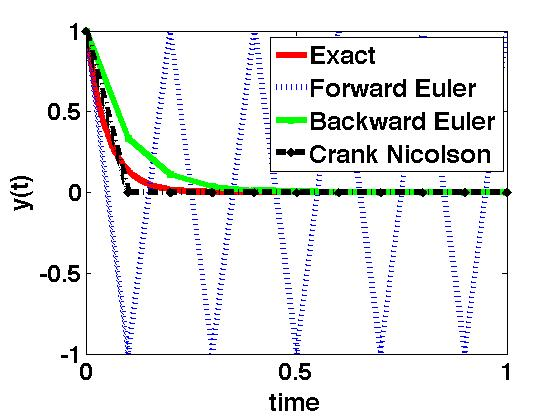
\includegraphics[scale=.4]{./Timestepping/unstable_forward_Euler.jpg}
\caption{A numerical solution to the ODE in eq.\ \eqref{eq:ODEstability} with $\lambda=20$ and with a timestep of $h=0.1$ demonstrating the instability of the Forward Euler method and the stability of the Backward Euler and Crank Nicolson methods.} \label{fig:ODEstability}
\end{center}
\end{figure}
Figure \ref{fig:ODEstability} above shows how both methods converge to the solution, but the forward Euler solution is unstable for the chosen timestep. Listing \ref{lst:MatlabInstability} is a Matlab program where you can play around with the value of $\lambda$ to see how, for a fixed timestep, this changes the stability of the method. 
\lstinputlisting[style=matlab_style,language=Matlab,label=lst:MatlabInstability,caption={A Matlab program to demonstrate instability of different timestepping methods.}]{./Timestepping/Programs/Simple_ODE_Example_of_Unstable_FE.m}

%%%%%%%
%Section
%%%%%%%
\section{Stability and Accuracy of Forward Euler, Backward Euler and Crank-Nicolson Time Stepping Schemes for $y'=-\lambda y$}

The examples discussed show that numerical stability is an important consideration when finding approximate solutions to differential equations on computers. Numerical stability requires a careful choice of numerical method and timestep for each numerical solution to a differential equation. We now try to understand these observations so that we have some guidelines to design numerical methods that are stable. The numerical solution to an initial value problem with a bounded solution is {\bf stable} if the numerical solution can be bounded by functions which are independent of the step size. There are two methods which are typically used to understand stability. The first method is linearized stability, which involves calculating eigenvalues of a linear system to see if small perturbations grow or decay. A second method is to calculate an energy like quantity associated with the differential equation and check whether this remains bounded. 

We shall assume that $\lambda\geq0$ so that the exact solution to the ODE does not grow without bound. The forward Euler method gives us
\begin{align*}
&{} \frac{y^{n+1}-y^n}{h}=-\lambda y^n
\\&{} y^{n+1}=(1-\lambda h)y^n
\\&{} \Rightarrow \lvert y^{n+1} \rvert \geq \lvert (1-\lambda h) \rvert \lvert y^n \rvert \quad \text{ if } \lvert (1-\lambda h) \rvert > 1
\\&{} \Rightarrow \lvert y^{n+1} \rvert \leq \lvert (1-\lambda h) \rvert \lvert y^n \rvert \quad \text{ if } \lvert (1-\lambda h) \rvert <1.
\end{align*}

We can do a similar calculation for backward Euler to get
\begin{align*}
&{} \frac{y^{n+1}-y^n}{h}=-\lambda y^{n+1}
\\&{} y^{n+1}=\frac{y^n}{1+\lambda h}
\\&{} \Rightarrow \lvert y^{n+1} \rvert \leq \left\lvert \frac{y^n}{1+\lambda h} \right\rvert \leq \lvert y^n \rvert \quad \text{ since } \left\lvert \frac{1}{1+\lambda h} \right\rvert <1.
\end{align*}
Thus, the backward Euler method is unconditionally stable, whereas the forward Euler method is not. We leave the analysis of the Crank-Nicolson method as an exercise.

A second method, often used to show stability for partial differential equations is to look for an energy like quantity and show that this bounds the solution and prevents it from becoming too positive or too negative. Usually, the quantity is chosen to be non negative, then all one needs to do is deduce there is an upper bound. We sketch how this is done for an ordinary differential equation so that we can use the same ideas when looking at partial differential equations. Recall that the forward Euler algorithm is given by
$$\frac{y^{n+1}-y^n}{h}=-\lambda y^n.$$
Multiplying this by $y^{n+1}$ we find that
\begin{align*}
&{} (y^{n+1})^2=(1-h\lambda)y^ny^{n+1}.
\end{align*}
Now to obtain a bound on $\lvert y^{n+1}\rvert$ in terms of $\lvert y^n \rvert$, we use the following fact
$$(a-b)^2\geq0\Rightarrow a^2+b^2\geq2ab\Rightarrow\frac{(y^{n+1})^2+(y^n)^2}{2}\geq y^ny^{n+1}.$$
Hence a sufficient condition for stability if 
$$(1-h\lambda)>0$$
is that
\begin{align*}
&{} (y^{n+1})^2\leq(1-h\lambda)\frac{(y^{n+1})^2+(y^n)^2}{2}
\\&{} (y^{n+1})^2\frac{1+h\lambda}{2}\leq\frac{1-h\lambda}{2}(y^n)^2
\\&{} (y^{n+1})^2\leq\frac{1-h\lambda}{1+h\lambda}(y^n)^2,
\end{align*}
thus if $1-h\lambda>0$, then $0<\frac{1-h\lambda}{1+h\lambda}<1$ and so we have stability, we again see that the algorithm is stable provided the timestep is small enough. There are many situations for which $\lambda$ is large and so the timestep, $h$ needs to be very small. In such a situation, the forward Euler method can be very slow on a computer.

Stability is not the only requirement for a numerical method to approximate the solution to an initial value problem. We also want to show that as the timestep is made smaller, the numerical approximation becomes better. For the forward Euler method we have that
\begin{align*}
  &{} \frac{y^{n+h}-y^{n}}{h}=-\lambda y^n
\end{align*}
now if
\begin{align*}
&{}y^n=y(t) \\
&{}y^{n+1}=y(t+h)
\end{align*}
then\footnote{We will use big `Oh' to mean that there exists a constant so that if $f~O(h)$, then for $h\rightarrow0$, we have that $\left|\frac{f}{h}\right|<C$, where $C$ is some constant.}
\begin{align*}
\\&y^{n+1}= y(t)+h\frac{\mathrm{d}y}{\mathrm{d}t} + O(h^2)
\end{align*}
so
\begin{align*}
\frac{y^{n+1}-y^n}{h}+\lambda y^n &{} = \frac{y(t+h)-y(t)}{h} +\lambda y(t)
\\&{} =\frac{\mathrm{d}y}{\mathrm{d}t} +O(h)+\lambda y(t)
\\&{} = O(h).
\end{align*}
We can do a similar calculation to show that the Crank-Nicolson method is second-order. In this case however, we use Taylor expansions around $y(t+h/2)$.
\begin{align*}
&{}\frac{y^{n+1}-y^n}{h}=-\lambda \frac{ y^{n+1} + y^n}{2}
\end{align*}
so
\begin{align*}
&{} y^{n+1} =y(t+h)=y(t+h/2)+(h/2)\frac{\mathrm{d}y}{\mathrm{d}t} +(h/2)^2\frac{1}{2}\frac{\mathrm{d}^2y}{\mathrm{d}t^2} + O(h^3)
\\&{} y^{n} =y(t)=y(t+h/2)-(h/2)\frac{\mathrm{d}y}{\mathrm{d}t} +(h/2)^2\frac{1}{2}\frac{\mathrm{d}^2y}{\mathrm{d}t^2} + O(h^3)
\end{align*}
hence
\begin{align*}
\frac{y^{n+1}-y^n}{h}+\lambda \frac{ y^{n+1} + y^n}{2} &{} =\frac{\mathrm{d}y}{\mathrm{d}t} + O(h^2) +\lambda \left[y(t+h/2)+O(h^2) \right]
\\&{} = O(h^2).
\end{align*}
Thus this is a second-order method.

%%%%%%%
%Section
%%%%%%%
\section{Exercises}
\begin{enumerate}
\item[1)] Determine the real values of $\lambda$ and timestep $h$ for which the implicit midpoint rule is stable for the ODE 
\begin{equation*}
\frac{\mathrm{d}y}{\mathrm{d}t}=-\lambda y
\end{equation*}
Sketch the stable region in a graph of $\lambda$ against timestep $h$.
\item[2)] Show that the backward Euler method is a first-order method.
\end{enumerate}


\chapter{One-Dimensional Discrete Fourier Transforms}
\footnote{For more detail, see Olver and Shakiban~\cite{OlvSha06}.} The discrete Fourier transform (DFT) takes a function sampled at a finite number of points and finds the coefficients for the linear combination of trigonometric polynomials that best approximates the function; the number of trigonometric polynomials used is equal to the number of sample points.  Suppose we have a function $f(x)$ which is defined on the interval $a \leq x \leq b$. Due to memory limitations, a computer can only store values at a finite number of sample points, i.e. $a \leq x_0 < x_1 < ... <x_n \leq b$. For our purposes these points will be equally spaced, for example $x_1-x_0=x_3-x_2$, and so we can write
\begin{eqnarray}
x_j = a +jh, \qquad j=0,1,2,...,n
\end{eqnarray}
where $x_j$ are the \emph{sample points}, $n$ is the number of sample points and
\begin{eqnarray}
 h=\frac{b-a}{n}.
\end{eqnarray}
It is convenient to use the \emph{standard interval}, for which $0 \leq x \leq 2\pi$. Rewriting $x$ in terms of standard interval yields
\begin{eqnarray}
x_0=0,x_1=\frac{2\pi}{n},x_2=\frac{4\pi}{n},x_j=\frac{2j\pi}{n},...,x_{n-1}=\frac{2(n-1) \pi}{n}
\end{eqnarray}
Notice how $x_n=2\pi$ is omitted;  periodicity implies that the value of the function at $2\pi$ is the same as the value of the function at $0$, so it need not be included. We will introduce the DFT using the language of linear algebra. Much of this formalism carries over to continuous functions that are being approximated. It also makes it easier to understand the computer implementation of the algorithms. Many computer packages and programs are optimized to perform calculations through matrix operations, so the formalism is also useful when actually calculating transforms. We write the approximation to $f(x)$ at the sample points as a finite dimensional vector
\begin{eqnarray}
\bm{f}=(f_0,f_1,...,f_{n-1})^{T}=(f(x_0),f(x_1), ... ,f(x_{n-1}))
\end{eqnarray}
where
\begin{eqnarray}
 f_j=f(x_j)=f \left(\frac{2 j \pi}{n} \right).
\end{eqnarray}
The DFT decomposes the sampled function $f(x)$ into a linear combination of complex exponentials, $\exp(ikx)$ where $k$ is an index. Since
\begin{eqnarray}
\exp(ikx)=\cos(kx)+i\sin(kx),
\end{eqnarray}
we also obtain an expansion in trigonometric functions, which may be more familiar from courses in calculus and differential equations. Since the function is sampled at $n$ points, the highest frequency of oscillation that can be resolved will have $n$ oscillations. Any frequencies higher than $n$ in the original function are not adequately resolved and cause an \emph{aliasing} error (see, for example, Boyd~\cite{Boy01} or Uecker~\cite{Uec09} for more on this). This error can be reduced by sampling at a greater number of points so that the number of approximating exponentials functions can also be increased. There is a tradeoff between increasing the accuracy of the simulation and the time required for the simulation to complete. For many cases of scientific and practical interest, simulations with up to thousands of grid points can be computed relatively quickly. Below we explain how a function $f(x)$ can be approximated by an interpolating trigonometric polynomial $p(x)$ so that 
\begin{eqnarray}
f(x) \approx p(x)=c_0+c_1e^{2ix}+c_2e^{2ix}+...+c_{n-1} e^{(n-1)ix}=\sum\limits_{k=0}^{n-1} c_k e^{ikx}
\end{eqnarray} 
The $\approx$ symbol means that $f(x)$ and $p(x)$ agree on each sample point, i.e., $f(x_j)=p(x_j)$ for each $j=0,1,...n-1$, but the interpolated polynomial $p(x)$ is only an approximation of the true solution $f(x)$ away from the sample points.. The $c_n$ are called discrete \emph{Fourier coefficients} and are what we will be looking to solve for. $p(x)$ represents the values of interpolating trigonometric polynomial of degree $\leq n-1$, so if we have the values of these coefficients then we have a function we can use as an approximation of $f(x)$. Since we are working in a finite-dimensional vector space, a useful approach is to rewrite the discrete Fourier series as a vector. We let
\begin{eqnarray}
\bm{\omega_k}&=&(e^{ikx_0},e^{ikx_1},e^{ikx_2},...,e^{ikx_n})^T \\
&=& (1,e^{2k \pi i/n},e^{4k\pi i/n},...,e^{2(n-1)k\pi i/n})^T,
\end{eqnarray}
where $k=0,1,...,n-1$. The interpolation conditions, $f(x_j)=p(x_j)$, can also be rewritten in vectorial form
\begin{eqnarray}\label{eq:FourExp}
\bm{f}=c_0\bm{\omega_0}+c_1\bm{\omega_1}+...+c_{n-1} \bm{\omega_{n-1}}.
\end{eqnarray}
Here $\bm f$ is a vector evaluated at the sample points, which is decomposed into vectors $\bm{\omega}_k$, much as a vector in three dimensional space can be decomposed into the components in the $x$, $y$ and $z$ directions. The DFT allows us to compute the coefficients $c_i$ given the value of the function at the sample points. This may at first seem unmotivated, but in many applications, such as solving differential equations, it is easier to manipulate a linear combination of trigonometric polynomials,  $\bm{\omega_0},...,\bm{\omega_{n-1}}$, than it is to work with the original function. In order to solve for $c_k$, we use the orthonormality of the basis elements $\bm{\omega_0},...,\bm{\omega_{n-1}}$. We now explain how this is done \footnote{For a more detailed explanation see Olver and Shakiban~\cite{OlvSha06}.}. 

Define $\xi_n=e^{2\pi i/n}$. We observe that 
\begin{equation}
\left(\xi_n\right)^n=\exp\left(\frac{2\pi i n}{n}\right)=\cos(2\pi ) +i\sin(2\pi )=1
\end{equation}
For this reason $\xi_n$ is known as the primitive $n^{\text{th}}$ root of unity. Note also that for $0\leq k < n$, we have that $(\xi_n^k)^n=1$, so all other roots of unity when taken to the power $n$ can be obtained from the primitive $n^{\text{th}}$ root of unity. We will use this to perform the DFT algorithm to calculate the coefficients $c_0,...,c_{k-1}$ in eq.\ \eqref{eq:FourExp}. The main idea behind the DFT algorithm is to use orthogonality of the vectors $\bm \omega_k$. To show the orthogonality between the vectors $\bm \omega_k$ and $\bm \omega_l$, we let $\bm \omega_l^*$ denote the complex conjugate of $\bm \omega_l$, and then take the inner product of $\bm \omega_k$ and $\bm \omega_l$ and find that
\begin{align*}
\left<\bm \omega_k, \bm \omega_l \right>&{}=\frac{1}{n}\sum_{m=0}^{n-1}\exp\left(\frac{2\pi ik m}{n}\right)\left[\exp(\frac{2\pi il m}{n})\right]^*
\\&{}=\frac{1}{n}\sum_{m=0}^{n-1}\exp\left(\frac{2\pi i(k-l) m}{n}\right)
\\&{}=\frac{1}{n}\sum_{m=0}^{n-1}\cos\left(\frac{\pi(k-l)m}{n}\right)+i\sin\left(\frac{\pi(k-l)m}{n}\right)
\\&{}=\left\{{1\quad\textup{if } k=l}\atop{0\quad\textup{otherwise}}\right.
\end{align*}
To deduce the last part, if $k=l$ then $\exp(0)=1$, and if $k\ne l$, then we are sampling the sine and cosine functions at equally spaced points on over an integral number of wavelengths. Since these functions have equal magnitude positive and negative parts, they sum to zero, much as the integral of a sine or cosine over an integral number of wavelengths is zero. This implies that we can compute the Fourier coefficients in the discrete Fourier sum by taking inner products 
\begin{eqnarray}
c_k=<\bm{f},\bm{\omega_k}>=\frac{1}{n} \sum\limits_{m=0}^{n-1} \xi_n^{-mk}f_j.
\end{eqnarray} 
We note the close connection between the continuous and discrete settings, where an integral is replaced by a sum.

%%%%%%%%
%subsection
%%%%%%%%
\section{Fast Fourier Transform}
Computing the Fourier coefficients, $c_0,...,c_{n-1}$ using the DFT from the definition can be very slow for large values of $n$. Computing the Fourier coefficients $c_0,...c_{n-1}$ requires $n^2-n$ complex multiplications and $n^2-n$ complex additions. In 1960, Cooley and Tukey~\cite{CooTuk65} rediscovered a much more efficient way of computing DFT by developing an algorithm known as the Fast Fourier Transforms (FFT) -- the method was known to Gauss, but received little attention since he did not publish it~\cite{HeiJohBur84}. The FFT cuts the number of arithmetic operations down to $O(n\log n)$. For large values of $n$, this can make a huge difference in computation time compared to the standard DFT. The reason why the FFT is so important is that it is heavily used in spectral methods. The basic FFT algorithm used by Cooley and Tukey~\cite{CooTuk65} is well documented in many places, however, there are other implementations of the algorithm and the best version of the algorithm to use depends heavily on computer architecture. We therefore do not give further descriptions here.

\chapter{Finding Derivatives using Fourier Spectral Methods}
Spectral methods are a class of numerical techniques that often utilize the FFT. Spectral methods can be implemented easily in Matlab, but there are some conventions to note. First note that Matlab's ``fft'' and ``ifft'' functions store wave numbers in a different order than has been used so far. The wave numbers in Matlab and in most other FFT packages are ordered, $0,1,...,\frac{n}{2},-\frac{n}{2}+1,-\frac{n}{2}+2,...,-1$. Secondly, Matlab does not take full advantage of real input data. The DFT of real data satisfies the symmetry property $\hat{v}(-k)=\hat{v}(k)$, so it is only necessary to compute half of the wave numbers. Matlab's ``fft" command does not take full advantage of this property and wastes memory storing both the positive and negative wave numbers. Third, spectral accuracy (exponential decay of the magnitude of the Fourier coefficients) is better for smooth functions, so where possible be sure your initial conditions are smooth -- \textbf{When using a Fourier spectral method this requires that your initial conditions are periodic}.
%%%%%%%%
% subsection
%%%%%%%%
\section{Taking a Derivative in Fourier Space}
Let $u(x)$ be a function which is sampled at the $n$ discrete points $x_i \in {h,2h,...,ih,..,2\pi-h,2\pi}$ and $h=2\pi/n$ in real space. Now take the FFT
\begin{eqnarray}
\text{FFT}(u_j) \equiv \hat{u}_k \qquad \text{where} \quad k \in {\frac{-n}{2}+1,...\frac{n}{2}}.
\end{eqnarray}
The Fourier transform of $\frac{\partial^2 u_j}{\partial x^2}$ can be easily computed from $\hat{u}_k$\footnote{More details can be found in Trefethen~\cite[Chap. 3]{Tre00}}:
\begin{eqnarray}
\textrm{FFT}(\frac{\partial^\nu u_j}{\partial x^\nu}) \equiv (ik)^\nu \hat{u}_k \qquad \text{where} \quad \hat{u}_{n/2}=0 \quad, \text{if \quad $\nu$ \quad \text{is odd}}. \label{eq:Spectral_Method_Deriv}
\end{eqnarray}
Thus, differentiation in real space becomes multiplication in Fourier space. We can then take the inverse fast Fourier Transform (IFFT) to yield a solution in real space. In the next section we will use this technique to implement forward Euler and backward Euler timestepping schemes to compute solutions for several PDEs.

%subsection
\subsection{Exercises}
\begin{enumerate}
\item[1)] Let $u(x)=\sum_k \hat{u}_k \exp(ikx)$ be the Fourier series representation of a function $u(x)$. Explain why 
$$\frac{\mathrm{d}^{\nu}u}{\mathrm{d}x^{\nu}}=\sum (ik)^{\nu}\hat{u}_k,$$
provided the series converges.
\item[2)] \footnote{This question was prompted by an REU and UROP project due to Sudarshan Balakrishan which is available at \url{http://www.math.lsa.umich.edu/undergrad/REU/projects.html}.} Consider the linear KdV equation
$$u_t+u_{xxx}=0$$
with periodic boundary conditions for $x\in(0,2\pi]$ and the initial data
\begin{align*}
&{} u(x,0)= \left\{{0\quad\textup{ if } 0< x\leq\pi}\atop{1\quad\textup{ if } \pi<x\leq2\pi }\right.
\end{align*}
\begin{enumerate}
\item[a)] Using separation of variables, show that the ``solution'' is
$$u(t,x)=\frac{1}{2}-\frac{2}{\pi}\sum_{j=0}^{\infty}\frac{\sin((2j+1)x-(2j+1)^3t)}{2j+1}.$$
Quotation marks are used because the expression for the solution that is given does not converge when differentiated either once in time or twice in space.
\item[b)] As explained by Olver~\cite{Olv10}, this solution has a fractal structure at times that are an irrational multiple of $\pi$ and a quantized structure at times that are rational multiples of $\pi$. The Matlab program in listing \ref{lst:DispQuant} uses the Fast Fourier transform to find a solution to the linearized KdV equation.  Explain how this program finds a solution to the linearized KdV equation.
\item[c)] Compare the numerical solution produced by the Matlab program with the analytical solution. Try to determine which is more accurate and see if you can find evidence or an explanation to support your suggestions.
\end{enumerate}

\lstinputlisting[style=matlab_style,label=lst:DispQuant,caption={A Matlab program which solves the linearized KdV equation using the Fast Fourier transform.}]{./FindingDerivatives/Programs/DispQuant.m}
 
\end{enumerate}

\chapter{Examples in Matlab}

We now want to find approximate numerical solutions using Fourier spectral methods. In this section we focus primarily on the heat equation with periodic boundary conditions for $x\in[0,2\pi)$. Many of the techniques used here will also work for more complicated partial differential equations for which separation of variables cannot be used directly.
%%%%%%%
%Section
%%%%%%%
\section{1D Heat Equation}
The 1D heat equation
\begin{eqnarray}\label{eq:heat}
\frac{\partial u}{\partial t} = \alpha \frac{\partial^2 u}{\partial x^2}
\end{eqnarray}
is a well known second order PDE for which exact series solutions can be found using separation of variables.  It arises in several contexts such as in predicting the temperature in a thin uniform cross section rod. The equation and its derivation can be found in introductory books on partial differential equations and calculus, for example \cite{BoyDip10}, \cite{CouJoh98} and \cite{HugEtAl08},   The constant $\alpha$ is the thermal diffusivity and $u(x,t)$ is temperature. We have already described how to solve the heat equation using separation of variables. Let us first discretize $x$ such that $x_j$ where $j=0,1,2,...,n$. $x_j$ are uniformly spteaced in $[0,2\pi)$. Let's now take the FFT of both sides of the 1D heat equation to obtain
\begin{eqnarray}
\widehat{\frac{\partial u}{\partial t}} = \alpha \widehat{\frac{\partial^2 u}{\partial x^2}}.
\end{eqnarray}
We then rewrite the spatial derivative using eq.\ \eqref{eq:Spectral_Method_Deriv} \footnote{The $k$ subscript denotes the coefficient of the k$^{th}$ Fourier mode.}
\begin{eqnarray}
\frac{\partial \hat{u}_k}{\partial t} = \alpha (ik)^2 \hat{u}_k, 
\end{eqnarray}
so that the partial differential equation now becomes a collection of independent ODEs. While we can solve these ODEs in time exactly, we will use techniques that will also allow us to obtain approximate solutions to PDEs we cannot solve exactly. We will discuss two methods for solving these ODEs, forward Euler and backward Euler.

%subsection
\subsection{Forward Euler}
Using the forward Euler method in time, we obtain
\begin{eqnarray}
\frac{\hat{u}_k^{n+1}-\hat{u}_k^n}{h} = \alpha (ik)^2 \hat{u}_k^n \\
\hat{u}_k^{n+1} =\hat{u}_{k}^n+\alpha h(ik)^2\hat{u}_k^n  
\end{eqnarray}
All that is left is to take the IFFT of the computed solution after all timesteps are taken to transfer it back to real space. This is a linear PDE, so only one IFFT is needed at the end. We will later see that this is different for a nonlinear PDE. A Matlab implementation of this is in listing \ref{lst:HeatFE1dMatlab}.

\lstinputlisting[style=matlab_style,label=lst:HeatFE1dMatlab,caption={A Matlab program to solve the heat equation using forward Euler timestepping.}]{./ExamplesInMatlab/Programs/Heat_Eq_1D_Spectral_FE.m}
 
 %subsection
\subsection{Backward Euler}
To derive this method, we start by applying the FFT and then perform timestepping using backward Euler. We then rewrite the implicit form into a form that gives the next iterate,
\begin{eqnarray}
\frac{\partial \hat{u}_k}{\partial t} &=& \alpha (ik)^2 \hat{u}_k \\
\frac{\hat{u}_k^{n+1}-\hat{u}_k^n}{h} &=& \alpha (ik)^2 \hat{u}_k^{n+1} \\
\hat{u}_k^{n+1}(1-\alpha h(ik)^2) &=&\hat{u}_k^n\\
\hat{u}_k^{n+1} &=&\frac{\hat{u}_k^n}{(1-\alpha h(ik)^2)}.
\end{eqnarray}
Below is a graph of the numerical solution to the heat equation\footnote{Methods to obtain the exact solution can be found in, among other places,  Boyce and DiPrima~\cite{BoyDip10}. } where $n=64$ obtained using the Matlab program in listing \ref{lst:HeatBE1dMatlab}. 
\begin{figure}
 \begin{center}
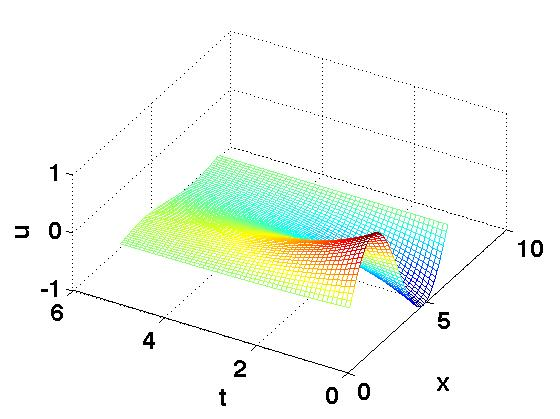
\includegraphics[scale=.35]{./ExamplesInMatlab/Heat_Equation_1D_BE_Color}
\caption{A numerical solution to the heat equation, eq.\ \eqref{eq:heat} computed using the backward Euler method.} \label{fig:HeatBE1dMatlab}
\end{center}
\end{figure}

\lstinputlisting[style=matlab_style,label=lst:HeatBE1dMatlab,caption={A Matlab program to solve the heat equation using backward Euler timestepping.}]{./ExamplesInMatlab/Programs/Heat_Eq_1D_Spectral_BE.m}

%subsection
\subsection{Exercises}
\begin{enumerate}
\item[1)] Write a program to solve the heat equation using the Crank-Nicolson method.
\item[2)] Solve the advection equation $u_t=u_x$ for $x\in[0,2\pi)$ with the initial data
\begin{enumerate}
\item[a)] $u(t=0,x)=\cos(x)$
\item[b)] $u(t=0,x)=\left\{{0\quad x<\pi}\atop{1\quad x\geq\pi}\right.$
\end{enumerate}
up to a time $T=1$. You can do this either by using separation of variables or by assuming that the solution is of the form $u(x,t)=f(x+t)$ and deducing what $f$ is in order to satisfy the initial conditions. In both cases please use the forward Euler, backward Euler and Crank-Nicolson timestepping schemes. After calculating the exact solution in each of these cases, examine how the maximum error at the final time depends on the timestep for each of these three methods.
\end{enumerate}


%%%%%%%
%Section
%%%%%%%
\section{Nonlinear Equations}
%subsection
\subsection{The 1D Allen-Cahn Equation}
So far we have dealt only with linear equations. Now it's time for a nonlinear PDE. The \emph{Allen-Cahn equation} models the separation of phases in a material. It was introduced by Sam Allen and J. W. Cahn~\cite{AllCah79}  and is 
\begin{eqnarray}
\frac{\partial u}{\partial t} = \epsilon\frac{\partial^2 u}{\partial x^2}+u-u^3, \label{eq:AllCah}
\end{eqnarray} 
where $\epsilon$ is a small but positive constant.  The way to numerically solve this is similar to the method used for the heat equation, but there are some notable differences. The biggest difference is that FFT($u^3$)$\neq$FFT($u$)$^3$, so the $u^3$ must be computed before taking the FFT. The FFT is a linear operation but cubing is non-linear operation, so the order matters
\begin{eqnarray}
\frac{\partial \hat{u}_k}{\partial t} = \epsilon\frac{\partial^2 \hat{u}_k}{\partial x^2}+\hat{u}_k-\widehat{u^3}_k. \label{Allen_Cahn_1D}
\end{eqnarray}
Next rewrite the first term on the right hand side, just like we did in the heat equation
\begin{eqnarray}
\frac{\partial \hat{u}_k}{\partial t} = \epsilon(ik)^2\hat{u}_k+\hat{u}_k-\widehat{u^3}_k.
\end{eqnarray}
In order to solve this numerically we are going to use a combination of implicit (backward Euler) and explicit (forward Euler) methods. We are going to skip forward Euler because it is unstable.

%subsubsection
\subsubsection{Implicit-Explicit Method} 
You might have already noticed that backward Euler is not going to work for the Allen-Cahn in its present state because of the nonlinear term. If you go to implement backward Euler you can see that you can't factor out all of the $\hat{u}_k^{n+1}$. Luckily there is a simple intuitive way around this that isn't detrimental to the accuracy of the solution. Write all the terms implicitly (backwards Euler) except for the nonlinear term which is expressed explicitly.  Applying this to Allen-Cahn we find that \footnote{Notice that when programming you are going to have to update the nonlinear term ($u^3$) each time you want to calculate the next timestep $n+1$. The reason this is worth mentioning is because for each timestep you are going to have to go from real space to Fourier space to real space, then repeat. For, the heat equation you can perform any number of timesteps in Fourier space and only convert back when you record your data.}
\begin{eqnarray}
\frac{\hat{u}_k^{n+1}-\hat{u}_k^n}{h} &=& \epsilon(ik)^2\hat{u}_k^{n+1}+\hat{u}_k^n-\widehat{(u^n)^3}_k \\
\hat{u}_k^{n+1}\left(-\epsilon(ik)^2+\frac{1}{h}\right)&=&\frac{1}{h}\hat{u}_k^n+\hat{u}_k^n-\widehat{(u^n)^3}_k \\
\hat{u}_k^{n+1}&=&\frac{\hat{u}_k^n(\frac{1}{h}+1)-\widehat{(u^n)^3}_k}{\left(-\epsilon(ik)^2+\frac{1}{h}\right)}. 
\end{eqnarray}
Now we have a form that we can work with. We can set the initial conditions to be $u(x,0)=\frac{1}{4} \sin(x)$ and plot the computed space-time evolution calculated by the Matlab code in listing \ref{lst:AllenCahnIE1dMatlab}. The computed result is in Fig.\ \ref{fig:AllenCahnIE1dMatlab}.

\lstinputlisting[style=matlab_style,label=lst:AllenCahnIE1dMatlab,caption={A Matlab program to solve the 1D Allen-Cahn equation using implicit explicit timestepping.}]{./ExamplesInMatlab/Programs/Allen_Cahn_1D_Spectral_IE.m}

\begin{figure}
\begin{center}
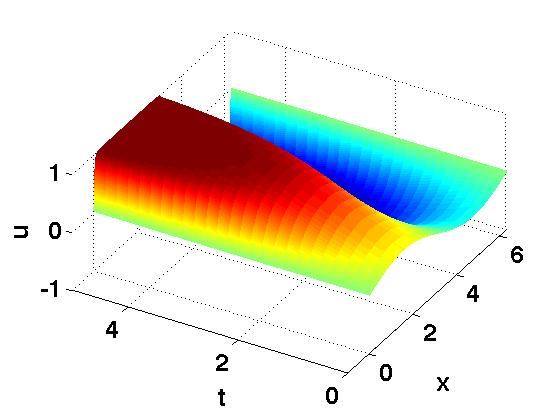
\includegraphics[scale=.2]{./ExamplesInMatlab/Allen_Cahn_BE_1D}
\caption{A numerical solution to the 1D Allen-Cahn equation, eq.\ \eqref{eq:AllCah}, with $\epsilon=0.001$ and $u(x,t=0)=0.25\sin(x)$ computed using an implicit explicit method.} \label{fig:AllenCahnIE1dMatlab}
\end{center}
\end{figure}

%subsection
\subsection{The 2D Allen-Cahn Equation}
Now we will look at the 2D form of the Allen-Cahn Equation, where $u(x,y,t)$ satisfies
\begin{eqnarray}
\frac{\partial u}{\partial t} = \epsilon\left(\frac{\partial^2 u}{\partial x^2}+\frac{\partial^2 u}{\partial y^2}\right)+u-u^3. \label{eq:AllCah2D}
\end{eqnarray}
The convert it into Fourier space by taking the FFT of both sides
\begin{eqnarray}
\frac{\partial \hat{u}_k}{\partial t} &=& \epsilon\left(\frac{\partial^2 \hat{u}_k}{\partial x^2}+\frac{\partial^2 \hat{u}_k}{\partial y^2}\right)+\hat{u}_k-\widehat{u^3}_k\\
\frac{\partial \hat{u}_k}{\partial t} &=& \epsilon\left((ik_x)^2\hat{u}_k+(ik_y)^2\hat{u}_k\right)+\hat{u}_k-\widehat{(u^3)}_k \label{eq:Allen_Cahn_2D}
\end{eqnarray}
where $k_x$ and $k_y$ is to remind us that we take the FFT in respected directions. We will also define
\begin{eqnarray}
f(u) \equiv u-u^3 \label{eq:nonlinear}
\end{eqnarray}
The way to deal with the first two terms on the right hand side is to take the FFT in the x-direction and then take it in the y-direction. The order in which the FFT is done, $x$ first or $y$ first is not important. Some software libraries offer a two dimensional FFT. It usually depends on the equation being solved whether it is more efficient to use a multidimensional FFT or many one dimensional FFTs. Typically, it is easier to write a program which uses a multidimensional FFT, but in some situations this is not very efficient since one can immediately reuse data that has just been Fourier transformed.
%subsubsection
\subsubsection{Implicit-Explicit Method}
In this method, the nonlinear term in eq.\ \eqref{eq:nonlinear} is calculated explicitly, while the rest of the terms will be written implicitly such that
\begin{align}
&{} \frac{\hat{u}_k^{n+1}-\hat{u}_k^n}{h} = \epsilon\left((ik_x)^2\hat{u}_k^{n+1}+(ik_y)^2\hat{u}_k^{n+1}\right)+\widehat{f(u^n)}_k 
\\&{} \hat{u}_k^{n+1}\left(-\epsilon(ik_x)^2-\epsilon(ik_y)^2+\frac{1}{h}\right)=\frac{\hat{u}_k^n}{h}+\widehat{f(u^n)}_k
\\&{} \hat{u}_k^{n+1} = \frac{\frac{\hat{u}_k^n}{h}+\widehat{f(u^n)}_k}{ \left(-\epsilon(ik_x)^2-\epsilon(ik_y)^2+\frac{1}{h}\right)}
\end{align}
we can then substitute in for $f(u)$
\begin{align}
\hat{u}_k^{n+1} = \frac{\hat{u}_k^n\left(\frac{1}{h}+1\right)-\widehat{(u^n)^3}_k}{ \left(-\epsilon(ik_x)^2-\epsilon(ik_y)^2+\frac{1}{h}\right)}. \label{eq:Allen_Cahn_IE_2D}
\end{align}
\begin{figure}
\begin{center}
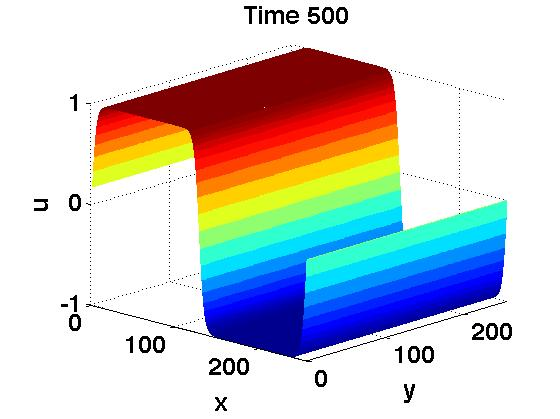
\includegraphics[scale=.2]{./ExamplesInMatlab/Allen_Cahn_2D_IE}
\caption{A numerical solution to the 2D Allen-Cahn equation, eq.\ \eqref{eq:AllCah2D} at time $t=500$ with $\epsilon=0.1$ and $u(x,y,t=0)=\sin(2\pi x)+0.001\cos(16\pi x)$ computed using an implicit explicit method.} \label{fig:AllenCahnIE2dMatlab}
\end{center}
\end{figure}
The Matlab code used to generate Fig.\ \ref{fig:AllenCahnIE2dMatlab} is in listing \ref{lst:AllenCahnIE2dMatlab}.

\lstinputlisting[style=matlab_style,label=lst:AllenCahnIE2dMatlab,caption={A Matlab program to solve the 2D Allen-Cahn equation using implicit explicit timestepping.}]{./ExamplesInMatlab/Programs/Allen_Cahn_2D_Spectral_IE.m}

%subsection
\subsection{Exercises}

Many of these exercises are taken from Uecker~\cite{Uec09}. Another introductory source of information on these equations is Trefethen and Embree~\cite{TreEmb01}.

\begin{enumerate}
\item[1)] Burgers equation is given by:
$$\frac{\partial u}{\partial t}=\nu \frac{\partial^2 u}{\partial x^2} - u\frac{\partial u}{\partial x}$$
where $\nu\in\mathbb{R}^+$ and $u$ has periodic boundary conditions. Solve this equation using an implicit-explicit method. If you take $\nu$ to be small, ensure that a sufficient number of grid points are used to get the correct numerical solution. A simple way to check this is to keep increasing the number of grid points and checking that there is no change in the solution. Another way to check this is to calculate the Fourier coefficients and check that the highest ones decay to machine precision. 
\item[2)] The Kuramoto-Sivashinsky equation is given by:
$$\frac{\partial u}{\partial t}=-\frac{\partial^2 u}{\partial x^2}-\frac{\partial^4 u}{\partial x^4}-u\frac{\partial u}{\partial x}$$
where $u$ has periodic boundary conditions.
\begin{itemize}
\item[a)] What does this equation model and what type of behavior do you expect its solutions to have?
\item[b)] Find numerical solutions to this equation using an implicit-explicit method.
\end{itemize}
\item[3)] The 1D Gray-Scott equations are given by:
$$\frac{\partial u}{\partial t}=d_1\frac{\partial^2 u}{\partial x^2}-uv^2+f(1-u),$$
$$\frac{\partial v}{\partial t}=d_2\frac{\partial^2 v}{\partial x^2} + uv^2 - (f+k)v$$
where $d_1$, $d_2$, $f$ and $k$ are constants. 
\begin{itemize}
\item[a)] What does this equation model and what type of behavior do you expect its solutions to have?
\item[b)] Find numerical solutions to this equation using an implicit-explicit method. Try several different values of $d_1$, $d_2$, $f$ and $k$ and compare the resulting patterns to what you can find in the literature.
\end{itemize}
\item[4)] The 2D Swift-Hohenberg equation is given by:
$$\frac{\partial u}{\partial t}=-\Delta^2u+2\Delta u+ (\alpha-1)u-u^3,$$
\begin{itemize}
\item[a)] What does this equation model and what type of behavior do you expect its solutions to have?
\item[b)] Find numerical solutions to this equation using an implicit-explicit method for several values of $\alpha$.
\end{itemize}
\item[5)] The 2D Gray-Scott equations are given by:
$$\frac{\partial u}{\partial t}=d_1\Delta u -uv^2+f(1-u)$$
$$\frac{\partial v}{\partial t}=d_2\Delta v  + uv^2 - (f+k)v$$
where $d_1$, $d_2$, $f$ and $k$ are constants. 
\begin{itemize}
\item[a)] What does this equation model and what type of behavior do you expect its solutions to have?
\item[b)] Find numerical solutions to this equation using an implicit-explicit method.
\end{itemize}
\item[6)] The 2D Complex Ginzburg-Landau equation is given by:
$$\frac{\partial A}{\partial t}=A+(1+i\alpha)\Delta A- (1+i\beta)|A|^2A.$$
An introductory tutorial to this equation can be found at \url{http://codeinthehole.com/static/tutorial/index.html}
\begin{itemize}
\item[a)] What does this equation model and what type of behavior do you expect its solutions to have?
\item[b)] Find numerical solutions to this equation using an implicit-explicit method for several values of $\alpha$ and $\beta$.
\end{itemize}
\end{enumerate}

\chapter{Nonlinear Ordinary Differential Equations and Iteration}

The implicit explicit method avoids the direct solution of nonlinear problems. This can be advantageous for some problems, but can also lead to severe time step restrictions in others. Furthermore, the resulting numerical schemes can sometimes have undesirable qualitative properties. For this reason, we need to describe methods that allow us to solve the nonlinear equations generated in fully-implicit numerical schemes. 

We consider an ordinary differential equation 
\begin{equation}
\frac{\mathrm{d}y}{\mathrm{d}t}=f(t,y) 
\end{equation}
for $t\in[t_{0},t^{*}]$, and for which $f(t,y)$ is not necessarily a linear function of $y$. We want to use an implicit numerical method to obtain an approximate solution of this problem -- for example backward Euler's method. If we want to demonstrate the convergence of the numerical scheme, we need to demonstrate convergence of functional iteration which we use to find the solution for the nonlinear equation term in using backward Euler's method. 

The results that follow are primarily taken from Iserles~\cite{Ise09}, although this material is also often found in calculus texts such as Lax, Burstein and Lax~\cite{LaxBurLax76}, and Hughes et al.~\cite{HugEtAl08}. We will let $t_{i}$ denote the time at time step $i$, $y_{i}$ denote the approximate solution at time step $i$ and $h$ denote the time step. We will assume $f$ is Lipschitz continuous, a condition that is weaker than differentiable but stronger than continuous, which we will give a precise definition of.  There are two classical iteration methods:
\begin{itemize}
\item fixed-point iteration 
\item Newton's (Newton-Raphson) method.
\end{itemize}
We will prove convergence of these two methods (a proof of the convergence of the modified Newton-Raphson method is in Iserles~\cite[p. 130]{Ise09}). We will analyze the specific problem $y'(t)=y^{2}$ with initial data
$y(0)=1$ and $t\in[0,0.99]$. 

%%%%%%%
%Section
%%%%%%%
\section{Exact Solution to an Example Nonlinear Ordinary Differential Equation}

We consider
\begin{equation}
\frac{\mathrm{d}y}{\mathrm{d}t}=y^{2}
\end{equation}
with initial data $y(t=0)=1$ and $t\in[0,0.99]$.  Whenever the solution $y(t)$ exists, it will be positive all the time, because the initial value is positive and $\frac{\mathrm{d}y}{\mathrm{d}t}$ is positive. 

To integrate this equation explicitly, we use separation of variables to find that
\begin{align}
&{}\int_{y(0)}^{y(t)}\frac{1}{\tilde{y}^{2}}\mathrm{d}\tilde{y}=\int_0^t\mathrm{d}\tau
\end{align}
which implies 
\begin{equation}
-\frac{1}{y(t)}=t+c
\end{equation}
where $c$ is the constant of integration. Using our initial data we get $c=-1$, so
\begin{equation}
y(t)=\frac{1}{1-t}
\end{equation}
is our exact solution for this problem. We will use this exact solution to compare the numerical solutions obtained by the different iterative methods. Notice that this exact solution becomes infinite as $t\rightarrow1$. 

%%%%%%%
%Section
%%%%%%%
\section{Definitions Required to Prove Convergence}

\begin{definition}{\bf The Lipschitz Condition}
A function $f(x):x\in D\subset\mathbb{R}$ is Lipschitz if $\left\Vert f(x_1)-f(x_2)\right\Vert \leq\lambda\left\Vert x_1-x_2\right\Vert $ for all $x_1$ and $x_2$ in the domain $D$.
\end{definition}

There are two specific definitions of the Lipschitz condition.

\begin{definition}{\bf Locally Lipschitz Condition}
The function $f(x)$ is called locally Lipschitz if, for each $z\in\mathbb{R}$, there exists an $L>0$ such that $f$ is Lipschitz on the open ball of center $z$ and radius $L$. 
\end{definition}

\begin{definition}{\bf Globally Lipschitz Condition}
If $f(x)$ is Lipschitz on all of the space $\mathbb{R}$ (i.e. The open ball is $\mathbb{R}$ in above definition), then $f$ is globally Lipschitz.
\end{definition}

Note the fundamental difference between the local and global versions of the Lipschitz-condition. Whereas in the local version the Lipschitz ``constant''($\lambda)$ and the open ball depend on each point $x\in\mathbb{R}$ , in the global version the ``constant''($\lambda)$ is fixed and the open ball is $\mathbb{R}$. In particular, a globally Lipschitz function is locally Lipschitz continuous, but the converse is not true.


%%%%%%%
% Section
%%%%%%%
\section{Existence and Uniqueness of Solutions to Ordinary Differential Equations}

Peano's theorem states that if $f(x)$ is continuous, then a solution to the ordinary differential equation $x'(t)=f(x)$ with initial condition $x(t_0)=x_0$ exists  at least in some neighbourhood of time $t_0$ -- this solution need not be unique. Picard's theorem states that if $f(x)$ is locally Lipschitz, then the solution for the ordinary differential equation $x'(t)=f(x)$ with initial condition $x(t_0)=x_0$ is unique when it exists. A comprehensive statement of these theorems is in Iserles~\cite[p. 445]{Ise09}, and there are proofs of these theorems in many books on ordinary differential equations (for example Birkhoff and Rota~\cite[Chap. 6, pg.\ 192]{BirRot89}). 
 
%%%%%%%
%Section
%%%%%%%
\section{Backward Euler}

We recall that the backward Euler method is given by
\begin{equation}
y^{n+1}=y^{n}+hf(y^{n+1}).
\end{equation}
Note that if $f$ is nonlinear, we need to solve a nonlinear equation in each step advancing the solution (numerical). It is usually hard to solve a nonlinear equation exactly using analytical methods, so we also use numerical methods.  For our example equation, we get
\begin{equation}
y^{n+1}=y^{n}+h\left(y^{n+1}\right)^2
\end{equation}
This example has the advantage that we can find its solutions algebraically, so we can then examine the behavior of numerical schemes.

%%%%%%%
%Section
%%%%%%%
\section{Convergence of Functional Iteration}

We often use functional iteration to solve nonlinear equations. We recall that there are two popular methods: fixed-point iteration and Newton's method.

%subsection
\subsection{Convergence of the Fixed-Point Method}

We want to find a root of $x=f(x).$ We try to use the fixed-point method and to construct a sequence $x_{n+1}=f(x_{n})$ where $n=0,1,2\ldots$.

\begin{theorem}
Let $f(x)$ have a fixed-point $\tilde{x}=f(\tilde{x})$, be Lipschitz continuous for $x\in(a, b)\subset\mathbb{R}$ with Lipschitz constant $k<1$ and $f(x)$ be continuous on $[a,b]$. Then the fixed point method $x_{n+1}=f(x_{n})$ converges to the unique fixed-point of $\tilde{x}=x_{\infty}=f(x_{\infty})$ for $x\in[a,b]$.
\end{theorem}

\begin{proof}
Since $f(x)$ is Lipschitz continuous, we find that, 
\begin{equation}
\left|x_{n+1}-x_{\infty}\right|=\left|f(x_{n})-f(x_{\infty})\right|\leq k\left|x_{n}-x_{\infty}\right|
\end{equation}
for $n=1,2\ldots$. Hence by induction we conclude that 
\begin{equation}
\left|x_{n+1}-x_{\infty}\right|\leq k^{n}\left|x_{1}-x_{\infty}\right|.
\end{equation}
Since $k<1$, $\lim_{n\rightarrow\infty}k^n\lvert x_1-x_{\infty}\rvert=0$, so we obtain a solution $x_{\infty}=f(x_{\infty})$, where $x_{\infty}$ is the fixed point. We can show that the limit is unique by supposing that there are two different limits and reaching a contradiction.\end{proof}

For a proof of the existence of the fixed-point under the assumptions used in this theorem, see a book on numerical analysis, such as Bradie~\cite{Bra06} or Iserles~\cite{Ise09}.

Regarding our problem, we apply fixed-point iteration, we want to find the root of an equation of the form:
\begin{equation}\label{eq:Fp}
w=hw^{2}+\beta=f(w). 
\end{equation}
When the timestep $h$ is small enough then $f'(w)=2hw\leq200h<1$. So fixed-point iteration is convergent provided the time-step is small enough. We note that eq.\ \eqref{eq:Fp} has two roots, and so the domain of the initial iterate plays an important role in determining which root is choosen.

%subsection
\subsection{Convergence of Newton's Method}

We now consider Newton's method. We want to find a root, $x^*$ of $f(x)$ such that $f(x^*)=0.$ Newton's method is a fixed-point method where the iterates are constructed by
\begin{equation}\label{eq:Newton}
x_{n+1}=x_{n}-\frac{f(x_{n})}{f'(x_{n})}
\end{equation}
where $n=0,1,2\ldots$. If the function $f(x)$ is sufficiently well behaved, then Newton's method has a quadratic rate of convergence. 

\begin{theorem}
Suppose $f(x)$ is twice continuously differentiable and that its second derivative is bounded. Suppose also that there exists $x^*$ for which $f(x^{*})=0$. Suppose $f'(x)\neq0$ in the interval $\left[x^{*}-\left|x^{*}-x_{0}\right|,x^{*}+\left|x^{*}-x_{0}\right|\right]$, $f''(x)$ is finite in the same interval and $\left\lvert x_{0} - x^{*}\right\rvert$ is small. Then, Newton's method is of quadratic convergence.
\end{theorem}

\begin{proof}
\begin{equation}
f(x^{*})=f(x_{n})+f'(x_{n})(x^{*}-x_{n})+\frac{1}{2!}f''(z_{n})(x^{*}-x_{n})^{2}
\end{equation}
by Taylor expansion with Lagrange form remainder. In the above $z_{n}\in[x_{n},x^{*}]$. Since $f(x^*)=0$, we have 
\begin{equation}
0=f(x_{n})+f'(x_{n})(x^{*}-x_{n})+\frac{1}{2!}f''(z_{n})(x^{*}-x_{n})^{2},
\end{equation}
so 
\begin{equation}
\frac{f(x_{n})}{f'(x_{n})}+(x^{*}-x_{n})=-\frac{1}{2!}\frac{f''(z_{n})}{f'(z_{n})}(x^{*}-x_{n})^{2}.
\end{equation}
Plug in the formula for $x_{n+1}$, from eq.\ \eqref{eq:Newton}  we have 
\begin{equation}
x^{*}-x_{n+1}=-\frac{1}{2!}\frac{f''(z_{n})}{f'(z_{n})}(x^{*}-x_{n})^{2}.
\end{equation}
Let
\begin{equation}
e_{n}=\left|x^{*}-x_{n}\right|.
\end{equation} 
We have 
\begin{equation}
e_{n+1}=\left|\frac{1}{2!}\frac{f''(z_{n})}{f'(z_{n})}\right|e_{n}^{2}
\end{equation}
and by our assumption, we know there is a constant $c$ such that
\begin{equation}
\left|\frac{1}{2!}\frac{f''(z_{n})}{f'(z_{n})}\right|<c.
\end{equation}
Hence we have $e_{n+1}<me_{n}^{2}$ for some finite constant $m$. So Newton's method is convergent provided $e_0=\lvert x_0-x^*\rvert$ is sufficiently small.
\end{proof}

Regarding our problem, we consider 
\begin{equation}
f(y)=y-hy^{2}-\beta.
\end{equation}
Hence $f'(y)=1-2hy\neq0$ and $f"(y)$ is finite, so our problem satisfies all assumptions if we choose our initial data and initial iterates suitably. Hence the Newton iterations will converge and give an approximation to the nonlinear term in backward Euler's method.

%%%%%%%
%Section
%%%%%%%
\section{Convergence of the Theta Method}

The backward Euler, forward Euler and Crank-Nicolson methods are special case of the theta method, so we will first prove the convergence of the theta method to encompass these three methods. The theta method is the following algorithm,
\begin{equation}
y^{n+1}=y^{n}+h[\theta f(t^{n},y^{n})+(1-\theta)f(t^{n+1},y^{n+1})]
\end{equation}
where
$n=0,1,\ldots$ and $\theta\in[0,1]$. Notice that for $\theta=1/2$ we obtain the Crank-Nicolson method or trapezoidal rule.

First, substituting the exact solution $y(t)$ and using the Taylor expansion we have
\begin{align}
&{}y(t^{n+1})-y(t^{n})-h[\theta f(t^{n},y(t^{n}))+(1-\theta)f(t^{n+1},y(t^{n+1}))]
\\&{}=y(t^{n+1})-y(t^{n})-h[\theta y'(t^{n})+(1-\theta)y'(t^{n+1})] \notag
\\&{} =[y(t^{n})+hy'(t^{n})+\frac{1}{2}h^{2}y''(t^{n})+\frac{1}{6}h^{3}y^{\prime\prime\prime}(t^{n})] \notag
\\&{}\hspace{2em}-y(t^{n})-h\{\theta y'(t^{n})+(1-\theta)[y'(t^{n})+hy''(t^{n})+\frac{1}{2}h^{2}y^{\prime\prime\prime}(t^{n})]\}+\mathcal{O}(h^{4}) \notag
\\&{}=\left(\theta-\frac{1}{2}\right)h^{2}y''(t^{n})+\left(\frac{1}{2}\theta-\frac{1}{3}\right)h^{3}y^{\prime\prime\prime}(t^{n})+\mathcal{O}(h^{4}). \notag
\end{align}
Subtracting the last expression from 
\begin{equation}
y^{n+1}-y^{n}-h[\theta f(t^{n},y^{n})+(1-\theta)f(t^{n+1},y^{n+1})]=0,
\end{equation}
we have that when $h$ is small enough
\begin{align}
&{}e^{n+1,h}
\\&{}=e^{n,h}+\theta h[f(t^{n},y(t^{n})+e^{n,h})-f(t^{n},y(t^{n}))] \notag
\\&{}\hspace{1em}+(1-\theta)h[f(t^{n+1},y(t^{n+1})+e^{n+1,h})-f(t^{n+1},y(t^{n+1}))] \notag
\\&{} \begin{cases}
-\frac{1}{12}h^{3}y^{\prime\prime\prime}(t^{n})+\mathcal{O}(h^{4}), & \theta=\frac{1}{2}\\
+(\theta-\frac{1}{2})h^{2}y''(t^{n})+\mathcal{O}(h^{3}), & \theta\neq\frac{1}{2}
\end{cases} \notag
\end{align} 
where $e^{i}=y^{i}-y(t^{i})$. Using the triangle inequality and by the Lipschitz continuity of $f$, there exist constants $c$ and $\lambda$ such that 
\begin{align}
&{}\left\Vert e^{n+1,h}\right\Vert
\\&{} \leq\left\Vert e^{n,h}\right\Vert +\theta h\lambda\left\Vert e^{n,h}\right\Vert +(1-\theta)h\lambda\left\Vert e^{n+1,h}\right\Vert +\begin{cases}
ch^{3} & \theta=\frac{1}{2}\\
ch^{2} & \theta\neq\frac{1}{2}
\end{cases}. \notag
\end{align}
When $\theta=\frac{1}{2}$, the theta method reduces to the trapezoidal rule. It is possible to show that the Crank-Nicolson method has second order convergence, see for example, Iserles~\cite{Ise09}. Now let's consider $\theta\neq\frac{1}{2}$, 
\begin{align}
&{}\left\Vert e^{n+1,h}\right\Vert \leq\frac{1+\theta h\lambda}{1-(1-\theta)h\lambda}\left\Vert e^{n,h}\right\Vert +\frac{c}{1-(1-\theta)h\lambda}h^{2}. 
\end{align}

We claim that 
\begin{equation}
\left\Vert e^{n,h}\right\Vert \leq\frac{c}{\lambda}\left[\left(\frac{1+\theta h\lambda}{1-(1-\theta)h\lambda}\right)^{n}-1\right]h
\end{equation}
We prove this statement by induction.  When $n=0$, $\left\Vert e^{n,h}\right\Vert =0$, since the initial conditions is exactly calculated. Now suppose this statement is true for $n=k$, where $k\geq0$ and is a integer. We want to show this statement is true for $n=k+1$. Consider
\begin{equation}
\left\Vert e^{k+1,h}\right\Vert \leq\frac{1+\theta h\lambda}{1-(1-\theta)h\lambda}\left\Vert e^{k,h}\right\Vert +\frac{c}{1-(1-\theta)h\lambda}h^{2},
\end{equation}
then plug in 
\begin{equation}
\left\Vert e^{kn,h}\right\Vert \leq\frac{c}{\lambda}\left[\left(\frac{1+\theta h\lambda}{1-(1-\theta)h\lambda}\right)^{k}-1\right]h.
\end{equation}
We have
\begin{align} 
&{} \left\Vert e^{k+1,h}\right\Vert 
\\&{} \leq\frac{c}{\lambda}\left[\left(\frac{1+\theta h\lambda}{1-(1-\theta)h\lambda}\right)^{k+1}-\frac{1+\theta h\lambda}{1-(1-\theta)h\lambda}\right]h+\frac{c}{1-(1-\theta)h\lambda}h^{2} \notag
\\&{}=\frac{c}{\lambda}\left[\left(\frac{1+\theta h\lambda}{1-(1-\theta)h\lambda}\right)^{k+1}-1\right]h. \notag
\end{align}
So our claim is true for all $n$ . Note that 
\begin{align}
\frac{1+\theta h\lambda}{1-(1-\theta)h\lambda} &{}=1+\frac{h\lambda}{1-(1-\theta)h\lambda} 
\\&{}\leq \exp\left(\frac{h\lambda}{1-(1-\theta)h\lambda}\right) \notag
\end{align}
by a Taylor expansion of the exponential function. Thus, we have
\begin{align}
\left\Vert e^{n,h}\right\Vert&{} \leq\frac{c}{\lambda}\left[\left(\frac{1+\theta h\lambda}{1-(1-\theta)h\lambda}\right)^{n}-1\right]h
\\&{}\leq\frac{c}{\lambda}\left(\frac{1+\theta h\lambda}{1-(1-\theta)h\lambda}\right)^{n}h \notag
\\&{}\leq\frac{ch}{\lambda}\exp\left(\frac{nh\lambda}{1-(1-\theta)h\lambda}\right). \notag
\end{align}
By our condition, $nh\leq t^{*}.$
Therefore 
\begin{equation}
\left\Vert e^{n,h}\right\Vert \leq\frac{ch}{\lambda}\exp\left(\frac{t^{*}\lambda}{1-(1-\theta)h\lambda}\right).
\end{equation}
So we have $\lim_{h\rightarrow0}\left\Vert e^{n,h}\right\Vert =0$ and $0\leq nh\leq t^{*}$. Hence the theta method is convergent
of order 1 when $\theta\neq\frac{1}{2}.$ 

Note that the backward Euler method is a special case of the theta method when $\theta=0$, so backward Euler's method is convergent of order 1. We arrive at our theorem.

\begin{theorem}
Backward Euler's method is convergent of order 1.
\end{theorem}

\begin{remark}
If $f$ is globally Lipschitz, then we can apply the above argument with respect to any time interval. If $f$ is only locally Lipschitz, then we need to analyze the situation more carefully. First, by Picard's theorem,  there is a unique solution of this ordinary differential equation for a short amount of time.  Indeed, we just need to know that the Lipschitz constant is finite without necessarily needing to know the exact value.
\end{remark}

\begin{remark} If one did not know of Picard's theorem, one could deduce the existence and uniqueness of solutions to ODEs by using time discretization.
\end{remark}

Now we consider $y'=y^{2}$ and $t\in[0,0.99]$. The exact solution of this problem is $y(t)=\frac{1}{1-t}$. So $1\leq y\leq100$. In our problem, $f=y^{2}$ is clearly analytic and it is locally Lipschitz. It is easy to show $f$ is not globally Lipschitz. If a function $f(x)$ is globally Lipschitz condition then there is a finite constant $\lambda$ such that 
\begin{equation}
\frac{\left\Vert f(x)-f(y)\right\Vert }{\left\Vert x-y\right\Vert }\leq\lambda
\end{equation}
for all $x,y\in \mathbb{R}$. In our problem, let $x=0$ and $\left\Vert y\right\Vert \rightarrow\infty,$ it is easy to check 
\begin{equation}
\frac{\left\Vert f(x)-f(y)\right\Vert }{\left\Vert x-y\right\Vert }\rightarrow\infty.
\end{equation}
We now discuss how one can find local Lipschitz constants $\lambda$. When $f$  is differentiable, we often just differentiate $f$ and find the maximum value of its derivative in the domain of interest. In our example, $f$ is simple and we only need to know that the Lipschitz constant is finite. So we use a more rough method to show that the Lipshitz constant is finite,
\begin{align}
&{}\left\Vert f(y^{1})-f(y^{2})\right\Vert 
=\left\Vert y^{1}+y^{2}\right\Vert \left\Vert y^{1}-y^{2}\right\Vert \leq\left(\left\Vert y^{1}\right\Vert +\left\Vert y^{2}\right\Vert\right)\left\Vert y^{1}-y^{2}\right\Vert. 
\end{align}
So it suffices to find the maximal value of $\left\Vert y\right\Vert$ in this problem. In our problem, $y(t)$ is continuous. Furthermore, $y(t)$ will be positive all the time, because the initial value is positive and $y'$ is positive. A continuous function has finite maximal value in a closed and bounded set. Note that the exact solution of our problem is $y(t)=\frac{1}{1-t}$ , so $1\leq y\leq100$. So we know that the Lipschitz constant in our problem is finite.

Finally, we get the convergence of functional iteration and backward Euler's method of our problem. Thus our numerical scheme for $y'=y^{2}$ with initial data $y(0)=1$ and $t\in[0,0.99]$ is convergent.

\begin{corollary}
By the theorems for existence and uniqueness of the solution for ordinary differential equations and Theorem 4.1 ,Theorem 4.2 and Theorem 4.3, we arrive at our final goal that the numerical solution generated by backward Euler's method with functional iteration exists and is unique when the time-step, $h0$ approaches zero.
\end{corollary}
 
\begin{remark} This requires careful choice of initial iterates when doing functional iteration.
\end{remark}

\begin{remark} Typically, the exact solution of an ODE is not known, although it is possible to deduce local Lipschitz continuity. Should the solution become infinite, a numerical method will either not converge or display very large values if the approximate solution closely approximates the exact solution. Some care is required in interpreting such numerical simulations in these cases.
\end{remark}
%%%%%%%
%Section
%%%%%%%
\section{Example Programs which use Iteration to Solve a Nonlinear Ordinary Differential Equation}

The following two Matlab programs demonstrate backward Euler's method for the example equation. The first one uses fixed-point iteration to solve for the nonlinear term and the second one uses Newton's method to solve for the nonlinear term. 

\lstinputlisting[style=matlab_style,language=Matlab,label=lst:BEFPiterMatlab,caption={A Matlab program to demonstrate fixed-point iteration.}]{./NonlinearOdeAndIteration/Programs/BackwardEulerFixedPoint.m}

\lstinputlisting[style=matlab_style,language=Matlab,label=lst:BENewIterMatlab,caption={A Matlab program to demonstrate Newton iteration.}]{./NonlinearOdeAndIteration/Programs/BackwardEulerNewtonIteration.m}
%%%%%%%
%  Section
%%%%%%%
\section{Exercises}
\begin{enumerate}
\item[1)] Run the fixed-point iteration program in Matlab and check that the outcome is reasonable. Now investigate how changing the number of time steps taken to go from a time of 0 to a time of 0.99, and the tolerance for fixed point iterations affects the maximum error. In particular try a range of 1,000-1,000,000 (in powers of 10) for the number of time steps and a tolerance ranging from $10^{-1}-10^{-7}$ (in powers of $10^{-1}$). You should observe that there is an ``ideal"  combination of subdivisions and tolerance to minimize the error. What are these combinations? Do this whole process again using Newton iteration instead. How have the answers changed?
\item[2)] Write a Matlab program to solve $y'=y^2$ with $y(0)=1$ using the Crank-Nicolson method and fixed point iteration. Explain why there are two fixed-points to which the fixed-point iteration can converge. Which of these fixed-points gives the correct approximation to the solution of the differential equation? Comment on how the choice of initial iterate for the fixed-point iteration determines the fixed-point to which the method converges. 
\item[3)] 
\begin{enumerate}
\item[a)] Show that the differential equation $y'=\sqrt{\lvert y\rvert}$, with $y(0)=0$ is not Lipschitz continuous. 
\item[b)] Find at least two analytical solutions to this differential equation.
\item[c)] Compute a numerical solution to this differential equations using the forward Euler method.
\item[d)] Compute a numerical solution to this differential equations using the backward Euler method. Be sure to try different initial guesses for the fixed-point iteration, not just the value at the previous time step; you should be able to calculate the influence of the choice of initial iterate on the selection of solution by the numerical method. Comment on this.
\item[e)] Compute a numerical solution to this differential equations using the implicit midpoint rule. Be sure to try different initial guesses for the fixed point iteration, not just the value at the previous time step; you should be able to calculate the influence of the choice of initial iterate on the selection of ``solution'' by the numerical method. Comment on this.
\item[f)] Repeat (d) and (e) with Newton iteration.
\item[g)] Comment on the applicability of numerical methods for solving differential equations without unique solutions.
\end{enumerate}
\item[4)] Modify the program for the 1-D Allen-Cahn equation so that it uses the Crank-Nicolson and fixed-point iteration for the nonlinear term. You will need to calculate the nonlinear term in real space, so that your resulting scheme is
\begin{equation}
\frac{\hat{u}^{n+1,k+1}-\hat{u}^n}{\delta t}=\frac{\hat{u}_{xx}^{n+1,k+1}+\hat{u}^n_{xx}}2 + \frac{1}{2}\widehat{\left[u^{n+1,k}- \left(u^{n+1,k} \right)^3\right]}+\frac{1}{2}\widehat{\left[u^{n}- \left(u^{n}\right)^3\right]},
\end{equation}
where $n$ denotes the time step and $k$ denotes the iterate. Stop the iterations once the maximum difference between successive iterates is sufficiently small.
\item[5)] Modify the program for the 2-D Allen-Cahn equation so that it uses the Crank-Nicolson method and fixed-point iteration for the nonlinear term. You will need to calculate the nonlinear term in real space.
\end{enumerate}

\chapter{Fortran Programs}

%%%%%%%
%  Section
%%%%%%%
\section{Example Programs}

To do parallel programming using OpenMP or MPI (Message passing interface), we typically need to use a lower level language than Matlab such as Fortran. Another possible choice of language is C, however Fortran has superior array handling capabilities compared to C, and has a similar syntax to Matlab, so is typically easier to use for scientific computations which make heavy use of regular arrays. It is therefore useful to introduce a few simple programs in Fortran before we begin studying how to create parallel programs. A good recent reference on Fortran is Metcalf, Reid and Cohen~\cite{MetReiCoh11}.  We recognize that most people will be unfamiliar with Fortran and probably more familiar with Matlab\footnote{Although Matlab is written in C, it was originally written in Fortran and so has a similar style to Fortran.}, C or C++, but we expect that the example codes will make it easy for anyone with some introductory programming background.   A recent guide which describes how to write efficient parallel Fortran code is Levesque and Wagenbreth\cite{LevWag11}. Our programs are written to be run on the Flux cluster at the University of Michigan. More information on this cluster can be found at \url{http://cac.engin.umich.edu/resources/systems/flux/} and at \url{http://cac.engin.umich.edu/started/index.html}. Below are four files you will need to run this.

\begin{enumerate}
\item[1)] A makefile to compile the Fortran code on Flux in listing \ref{lst:MakefileHeat}. This should be saved as {\it makefile}. Before using the makefile to compile the code, you will need to type\\
\texttt{module load fftw/3.2.1-intel}\\
at the command line prompt once logged into Flux. Then place the makefile and heat.f90 in the same directory, the example files below assume this directory is\\
\texttt{\${HOME}/ParallelMethods/Heat}\\
 and type\\
\texttt{make}\\
to compile the file. Once the file is compiled type\\
\texttt{qsub fluxsubscript}\\
to get the cluster to run your program and then output the results. The programs that follow use the library FFTW to do the fast Fourier Transforms. More information on this library can be found at \url{http://www.fftw.org/}.

\lstinputlisting[style=make_style,language=make,label=lst:MakefileHeat,caption={An example makefile for compiling a Fourier spectral Fortran heat equation program.}]{./FortranPrograms/Programs/FortranHeatEquation/makefile}

\item[2)] The Fortran program in listing \ref{lst:FortranHeat} -- this should be saved as {\it heat.f90}
\lstinputlisting[style=fortran_style,language=Fortran,label=lst:FortranHeat,caption={A Fortran Fourier spectral program to solve the heat equation using backward Euler timestepping.}]{./FortranPrograms/Programs/FortranHeatEquation/heat.f90}

\item[3]) An example submission script to use on the cluster in Listing \ref{lst:Fluxsubheat} -- this should be saved as {\it fluxsubscript}. More examples can be found at \url{http://cac.engin.umich.edu/resources/software/pbs.html}. To use it, please change the email address from \url{your_uniqname@umich.edu} to an email address at which you can receive notifications of when jobs start and are finished. 

\lstinputlisting[style=bash_style,language=bash,label=lst:Fluxsubheat,caption={An example submission script for use on Flux.}]{./FortranPrograms/Programs/FortranHeatEquation/fluxsubscript}

\item[4)] A Matlab plotting script\footnote{For many computational problems, one can visualize the results with 10-100 times less computational power than was needed to generate the results, so for problems which are not too large, it is much easier to use a high level language like Matlab to post-process the data.} to generate Fig.\ \ref{fig:FortranHeat} is in listing \ref{lst:PlotMatlab}.

\lstinputlisting[style=matlab_style,label=lst:PlotMatlab,caption={A Matlab program to plot the computed results.}]{./FortranPrograms/Programs/FortranHeatEquation/plotcreate.m}

\begin{figure}
\begin{center}
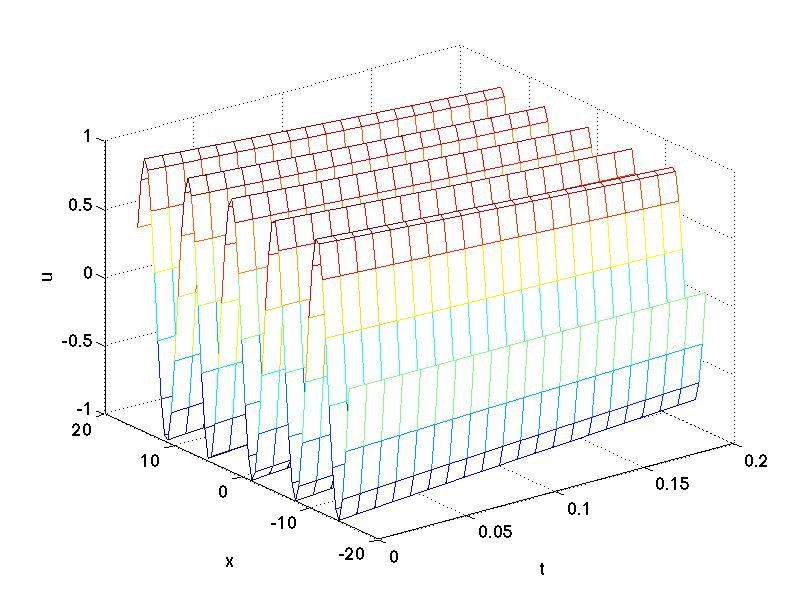
\includegraphics[scale=.35]{./FortranPrograms/heatPlot.jpg}
\caption{The solution to the heat equation computed by Fortran and post-processed by Matlab.} \label{fig:FortranHeat}
\end{center}
\end{figure}

\end{enumerate}


%%%%%%%
%  Section
%%%%%%%
\section{Exercises}
\begin{enumerate}
\item[1)] Please read the resources on the web page \url{http://cac.engin.umich.edu/started/index.html} to learn how to use the Flux cluster.
\item[2)] Modify the Fortran program for the 1-D heat equation to solve the Allen-Cahn equation, with your choice of time stepping scheme. Create a plot of the output of your run. Include the source code and plot in your solutions.
\item[3)] Modify the Fortran program for the 1-D heat equation to solve the  2-D heat equation with your choice of time stepping scheme. Your program should save the field at each time step rather than putting all the fields in a single large array. Create a plot of the initial and final states of your run. Include the source code and plots in your solutions.
\end{enumerate}


\chapter{Introduction to Parallel Programming}
%%%%%%%
% Section
%%%%%%%
\section{Overview of OpenMP and MPI}

To solve large computational problems quickly, it is necessary to take advantage of multiple cores on a CPU (central processing units) and multiple CPUs. Most programs written up until now are sequential and compilers will not typically automatically generate parallel executables,  so programmers need to modify the original serial computer code to take advantage of extra processing power. Two standards which specify what libraries that allow for parallel programming should do are OpenMP and MPI (the message passing interface). In this section, we cover the minimal amount of information required to understand, run and modify the programs in this tutorial. More detailed tutorials can be found at \url{https://computing.llnl.gov/tutorials/} and at \url{http://www.citutor.org}.

OpenMP is used for parallel programming on shared memory architectures -- each compute process has a global view of memory. It allows one to incrementally parallelize an existing Fortran, C or C++ code by adding directives to the original code. It is therefore easy to use. However some care is required in getting good performance when using OpenMP. It is easy to add directives to a serial code, but thought is required in creating a program which will show improved performance and give correct results when made to run in parallel. For the numerical solution of multidimensional partial differential equations on regular grids, it is easy to perform efficient and effective loop based parallelism, so a complete understanding of all the features of OpenMP is not required. OpenMP typically allows one to use 10's of computational cores, in particular allowing one to take advantage of multicore laptops, desktops and workstations.

MPI is used for parallel programming on distributed-memory architectures -- when separate compute processes have access to their own local memory and processes must explicitly receive data held in memory belonging to other processes which have sent the data. MPI is a library which allows one to parallelize Fortran, C and C++ programs by adding function calls which explicitly move data from one process to another. Careful thought is required in converting a serial program to a parallel MPI program because the data needs to be decomposed onto different processes, so it is usually difficult to incrementally parallelize a program that uses MPI. The best way to parallelize a program which will use MPI is problem dependent. When solving large problems, one typically does not have enough memory on each process to simply replicate all the data. Thus one wants to split up the data (known as domain decomposition) in such a way as to minimize the amount of message passing that is required to perform a computation correctly. Programming this can be rather complicated and time consuming. Fortunately, by using the 2DECOMP{\&}FFT library~\cite{LiLai10,LaiLi11} which is written on top of MPI, we can avoid having to program many of the data passing operations when writing Fourier spectral codes and still benefit from being able to solve partial differential equations on up to O($10^5$) processor cores.

%%%%%%%
% Section
%%%%%%%
\section{OpenMP}
Please read the tutorial at \url{https://computing.llnl.gov/tutorials/openMP/}, then answer the following questions:

%subsection
\subsection{OpenMP Exercises}
\begin{enumerate}
\item[1)] What is OpenMP?
\item[2)] Download a copy of the latest OpenMP specifications from \url{www.openmp.org}. What version number is the latest specification?
\item[3)] Explain what each of the following OpenMP directives does:
\begin{enumerate}
\item[i)] !\$OMP PARALLEL
\item[ii)] !\$OMP END PARALLEL
\item[iii)] !\$OMP PARALLEL DO
\item[iv)] !\$OMP END PARALLEL DO
\item[v)] !\$OMP BARRIER
\item[vi)] !\$OMP MASTER
\item[vii)] !\$OMP END MASTER
\end{enumerate}
\item[4)] Try to understand and then run the Hello World program in listing \ref{lst:ForOmpHw}  on 1, 2, 6 and 12 threads. Put the output of each run in your solutions, the output will be in a file of the form\\ 
\texttt{helloworld.o**********}\\
where the last entries above are digits corresponding to the number of the run. An example makefile to compile this on Flux is in listing \ref{lst:MakefileOmpHw}. An example submission script is in listing \ref{lst:Fluxsubhelloworld}. To change the number of OpenMP processes that the program will run on from say 2 to 6,  change \\
\texttt{ppn=2}\\ 
to\\ 
\texttt{ppn=6}\\
and also change the value of the OMP\_NUM\_THREADS variable from\\
\texttt{OMP\_NUM\_THREADS=2}\\
to \\
\texttt{OMP\_NUM\_THREADS=6}\\
On Flux, there is a maximum of 12 cores per node, so the largest useful number of threads for most applications is 12.

\lstinputlisting[style=fortran_style,language=Fortran,label=lst:ForOmpHw,caption={A Fortran program taken from \url{http://en.wikipedia.org/wiki/OpenMP}, which demonstrates parallelism using OpenMP.}]{./IntroductionToParallelProgramming/Programs/Helloworld/helloworld.f90}

\lstinputlisting[style=make_style,language=make,label=lst:MakefileOmpHw,caption={An example makefile for compiling the helloworld program in listing \ref{lst:ForOmpHw}.}]{./IntroductionToParallelProgramming/Programs/Helloworld/makefile}

\lstinputlisting[style=bash_style,language=bash,label=lst:Fluxsubhelloworld,caption={An example submission script for use on Flux.}]{./IntroductionToParallelProgramming/Programs/Helloworld/fluxsubscript}

\item[5)] Add OpenMP directives to the loops in the 2-D heat equation solver. Run the resulting program on 1,3,6 and 12 threads and record the time it takes to the program to finish. Make a plot of the final iterate.
\end{enumerate}
%%%%%%%
% Section
%%%%%%%
\section{MPI}

A copy of the current MPI standard can be found at \url{http://www.mpi-forum.org/}. It allows for parallelization of Fortran, C and C++ programs. There are newer parallel programming languages such as Co-Array Fortran (CAF) and Unified Parallel C (UPC) which allow the programmer to view memory as a single addressable space even on a distributed-memory machine. However, computer hardware limitations imply that most of the programming concepts used when writing MPI programs will be required to write programs in CAF and UPC. Compiler technology for these languages is also not as well developed as compiler technology for older languages such as Fortran and C, so at the present time, Fortran and C dominate high performance computing.  An introduction to the essential concepts required for writing and using MPI programs can be found at \url{http://www.shodor.org/refdesk/Resources/Tutorials/}. More information on MPI can be found in Gropp, Lusk and Skjellum~\cite{GroLusSkj99}, Gropp, Lusk and Thakur~\cite{GroLusTha99} and at \url{https://computing.llnl.gov/tutorials/mpi/}. There are many resources available online, however once the basic concepts have been mastered, what is most useful is an index of MPI commands, usually a search engine will give you sources of listings, however we have found the following sites useful:
\begin{itemize}
\item \url{http://www.mpi.forum.org/docs/mpi-11-html/node182.html}
\item \url{http://publib.boulder.ibm.com/infocenter/zos/v1r13/index.jsp?topic=\%2Fcom.ibm.zos.r13.fomp200\%2Fipezps00172.htm}
\item \url{http://www.open-mpi.org/doc/v1.4/}
\end{itemize}

% subsection
\subsection{MPI Exercises}
\begin{enumerate}
\item[1)] What does MPI stand for?
\item[2)] Please read the tutorials at \url{http://www.shodor.org/refdesk/Resources/Tutorials/BasicMPI/} and at \url{https://computing.llnl.gov/tutorials/mpi/}, then explain what the following commands do:
\begin{itemize}
\item \texttt{USE mpi} or \texttt{INCLUDE 'mpif.h'} 
\item \texttt{MPI\_INIT}
\item \texttt{MPI\_COMM\_SIZE}
\item \texttt{MPI\_COMM\_RANK}
\item \texttt{MPI\_FINALIZE}
\end{itemize}
\item[3)] What is the version number of the current MPI standard?
\item[3)] Try to understand the Hello World program in listing \ref{lst:ForMpiHw}. Explain how it differs from \ref{lst:ForOmpHw}. Run the program in listing \ref{lst:ForMpiHw} on 1, 2, 6, 12 and 24 MPI processes\footnote{One can run this program on many more than 24 processes, however, the output becomes quite excessive}. Put the output of each run in your solutions, the output will be in a file of the form\\ 
\texttt{helloworld.o**********}\\
where the last entries above are digits corresponding to the number of the run. An example makefile to compile this on Flux is in listing \ref{lst:MakefileMpiHw}. An example submission script is in listing \ref{lst:FluxsubhelloworldMpi}. To change the number of MPI processes that the program will run on from say 2 to 6,  change \\
\texttt{ppn=2}\\ 
to\\ 
\texttt{ppn=6}\\
and also change the submission script from\\
\texttt{mpirun -np 2 ./helloworld}\\ 
to\\ 
\texttt{mpirun -np 6 ./helloworld}.

On Flux, there is a maximum of 12 cores per node, so if more than 12 MPI processes are required, one needs to change the number of nodes as well. The total number of cores required is equal to the number of nodes multiplied by the number of processes per node. Thus to use 24 processes change  \\
\texttt{nodes=1:ppn=2}\\ 
to\\ 
\texttt{nodes=2:ppn=12}\\
and also change the submission script from\\
\texttt{mpirun -np 2 ./helloworld}\\ 
to\\ 
\texttt{mpirun -np 24 ./helloworld}.

\lstinputlisting[language=Fortran,label=lst:ForMpiHw,caption={A Fortran program which demonstrates parallelizm using MPI.}]{./IntroductionToParallelProgramming/Programs/HelloworldMpi/helloworld.f90}

\lstinputlisting[language=make,label=lst:MakefileMpiHw,caption={An example makefile for compiling the helloworld program in listing \ref{lst:ForMpiHw}.}]{./IntroductionToParallelProgramming/Programs/HelloworldMpi/makefile}

\lstinputlisting[language=bash,label=lst:FluxsubhelloworldMpi,caption={An example submission script for use on Flux.}]{./IntroductionToParallelProgramming/Programs/HelloworldMpi/fluxsubscript}

\end{enumerate}

\section{A first parallel program: Monte Carlo Integration}

To introduce the basics of parallel programming in a context that is a little more complicated than {\it Hello World}, we will consider Monte Carlo integration. We review important concepts from probability and Riemann integration, and then give example algorithms and explain why parallelization may be helpful.

\subsection{Probability}

\begin{definition} $f:U\subset \mathbb{R}^2 \rightarrow \mathbb{R}_+$ is a {\bf probability density function} if
$$ \int\int_U f \mathrm{d}A =1$$
\end{definition}

\begin{definition} If $f$ is a probability density function which takes the set $U\subset\mathbb{R}^2$, then the probability of events in the set $W\subset U$ occurring is
$$P(W)=\int\int_W f \mathrm{d}A.$$
\end{definition}

\begin{example} The joint density for it to snow $x$ inches tomorrow and for Kelly to win $y$ dollar in the lottery tomorrow is given by
$$f=\frac{c}{(1+x)(100+y)}$$
for
$$x,y\in [0,100]\times[0,100]$$
and $f=0$ otherwise. Find $c$.
\end{example}
 
\begin{definition} Suppose $X$ is a random variable with probability density function $f_1(x)$ and $Y$ is a random variable with a probability density function $f_2(y)$. Then $X$ and $Y$ are {\bf independent random variables} if their joint density function is
$$f(x,y)=f_1(x)f_2(y).$$
\end{definition}

\begin{example} The probability it will snow tomorrow and the probability Kelly will win the lottery tomorrow are independent random variables.
\end{example}

\begin{definition} If $f(x,y)$ is a probability density function for the random variables $X$ and $Y$, the {\bf X mean} is
$$\mu_1=\bar{X}=\int\int xf\mathrm{d}A$$
and the {\bf Y mean} is
$$\mu_2=\bar{Y}=\int\int yf\mathrm{d}A.$$
\end{definition}

\begin{remark} The X mean and the Y mean are the expected values of X and Y.
\end{remark}

\begin{definition} If $f(x,y)$ is a probability density function for the random variables $X$ and $Y$, the {\bf X variance} is
$$\sigma_1^2=\overline{(X-\bar{X})^2}=\int\int (x-\bar{X})^2f\mathrm{d}A$$
and the {\bf Y variance} is
$$\sigma_2^2=\overline{(Y-\bar{Y})^2}=\int\int (y-\bar{Y})^2f\mathrm{d}A.$$
\end{definition}

\begin{definition} The standard deviation is defined to be the square root of the variance.
\end{definition}

\begin{example} Find an expression for the probability that it will snow more than 1.1 times the expected snowfall and also that Kelly will win more than 1.2 times the expected amount in the lottery.
\end{example}

\subsection{Exercise}
\begin{itemize}
\item[1)] A class is graded on a curve. It is assumed that the class is a representative sample of the population, the probability density function for the numerical score $x$ is given by
$$ f(x)=C\exp\left(-\frac{(x-\mu)^2}{2\sigma^2}\right).$$
For simplicity we assume that $x$ can take on the values $-\infty$ and $\infty$, though in actual fact the exam is scored from $0$ to $100$. 
\begin{enumerate}
\item[a)] Determine $C$ using results from your previous homework.
\item[b)] Suppose there are 240 students in the class and the mean and standard deviation for the class is not reported. As an enterprising student, you poll 60 of your fellow students (we shall suppose they are selected randomly).  You find that the mean for these 60 students is 55\% and the standard deviation is 10\%. Use the Student's t distribution \url{http://en.wikipedia.org/wiki/Student\%27s_t-distribution} to estimate the 90\% confidence interval for the actual sample mean. Make a sketch of the t-distribution probability density function and shade the region which corresponds to the 90\% confidence interval for the sample mean.\footnote{The Student's t distribution is implemented in many numerical packages such as Maple, Mathematica, Matlab, R, Sage etc., so if you need to use to obtain numerical results, it is helpful to use on of these packages.} 
\end{enumerate}

{\bf Remark} Fortunately, all the students are hard working, so the possibility of a negative score, although possible, is extremely low, and so we neglect it to make the above computation easier.
\end{itemize}

\subsection{Riemann Integration}

Recall that we can approximate integrals by Riemann sums. There are many integrals one cannot evaluate analytically, but for which a numerical answer is required. In this section, we shall explore a simple way of doing this on a computer. Suppose we want to find 
$$I2d=\int_0^1\int_0^4 x^2+2y^2\mathrm{d}y\mathrm{d}x.$$
If we do this analytically we find
$$I2d=44.$$
Let us suppose we have forgotten how to integrate, and so we do this numerically. We can do so using the following Matlab code:
\lstinputlisting[language=Matlab,label=lst:MatlabInt,caption={A Matlab program which demonstrates how to approximate an integral by a sum.}]{./IntroductionToParallelProgramming/Programs/RiemannSum.m}

We can do something similar in three dimensions. Suppose we want to calculate
$$I3d=\int_0^1\int_0^1\int_0^4 x^2+2y^2+3z^2\mathrm{d}z\mathrm{d}y\mathrm{d}x.$$
Analytically we find that
$$I3d=68$$
\subsection{Exercises}
\begin{enumerate}
\item[1)] Modify the Matlab code to perform the three dimensional integral.
\item[2)] Try and determine how the accuracy of either the two or three dimensional method varies as the number of subintervals is changed.
\end{enumerate}

\subsection{Monte Carlo Integration}

\footnote{This section is taken from Chapter 3 of \underline{Vector Calculus} by Michael Corral which is available at \url{http://www.mecmath.net/} and where Java and Sage programs for doing Monte Carlo integration can be found.} It is possible to extend the above integration schemes to higher and higher dimensional integrals. This can become computationally intensive and an alternate method of integration based on probability is often used. The method we will discuss is called the \emph{Monte Carlo method}. The idea behind it is based on the concept of the \emph{average value} of a function, which you learned in single-variable calculus. Recall that for a continuous function $f(x)$, the \textbf{average value} $\bar{f}$ of $f$ over an interval $\lbrack a,b \rbrack$ is defined as \index{Monte Carlo method}\index{average value}
\begin{equation}\label{eqn:favg}
 \bar{f} ~=~ \frac{1}{b-a}\int_a^b f(x)\,dx ~.
\end{equation}

The quantity $b-a$ is the length of the interval $\lbrack a,b \rbrack$, which can be thought of as the ``volume'' of
the interval. Applying the same reasoning to functions of two or three variables, we define the \textbf{average
value} of $f(x,y)$ over a region $R$ to be
\begin{equation}\label{eqn:favg2}
 \bar{f} ~=~ \frac{1}{A(R)}\iint\limits_{R} f(x,y)\,dA ~,
\end{equation}
where $A(R)$ is the area of the region $R$, and we define the \textbf{average
value} of $f(x,y,z)$ over a solid $S$ to be
\begin{equation}\label{eqn:favg3}
 \bar{f} ~=~ \frac{1}{V(S)}\iiint\limits_{S} f(x,y,z)\,dV ~,
\end{equation}
where $V(S)$ is the volume of the solid $S$. Thus, for example, we have
\begin{equation}\label{eqn:favgint2}
 \iint\limits_{R} f(x,y)\,dA ~=~ A(R)\bar{f} ~.
\end{equation}
The average value of $f(x,y)$ over $R$ can be thought of as representing the sum of all the values of $f$ divided by
the number of points in $R$. Unfortunately there are an infinite number (in fact, \emph{uncountably} many) points
in any region, i.e. they can not be listed in a discrete sequence. But what if we took a
very large number $N$ of \emph{random} points in the region $R$ (which can be generated by a computer) and then took the
average of the values of $f$ for those points, and used that
average as the value of $\bar{f}$? This is exactly what the Monte Carlo method does. So in formula (\ref{eqn:favgint2})
the approximation we get is
\begin{equation}\label{eqn:monte}
 \iint\limits_{R} f(x,y)\,dA ~\approx~ A(R)\bar{f} \pm A(R)\sqrt{\frac{\overline{f^2} - (\bar{f})^2}{N}} ~,
\end{equation}
where
\begin{equation}
 \bar{f} ~=~ \frac{\sum_{i=1}^N f(x_i,y_i)}{N} \quad \text{and} \quad \overline{f^2} ~=~
 \frac{\sum_{i=1}^N (f(x_i,y_i))^2}{N} ~,
\end{equation}
with the sums taken over the $N$ random points $(x_1,y_1)$, $\ldots$, $(x_N,y_N)$.
The $\pm$ ``error term'' in formula (\ref{eqn:monte}) does not really provide
hard bounds on the approximation. It represents a single \emph{standard deviation} from the \emph{expected} value of the
integral. That is, it provides a \emph{likely} bound on the error. Due to its use of random points, the Monte Carlo
method is an example of a \emph{probabilistic} method (as opposed to \emph{deterministic} methods such as the Riemann sum approximation method, which use a specific formula for generating points).

For example, we can use the formula in eq.\ \eqref{eqn:monte} to approximate the volume $V$ under the surface $z=x^2+2y^2$ over the
rectangle $R =(0,1)\times(0,4)$. Recall that the actual volume is $44$. Below is a  Matlab code  that calculates the volume using Monte Carlo integration

\lstinputlisting[language=Matlab,label=lst:MatlabMC,caption={A Matlab program which demonstrates how to use the Monte Carlo method to calculate the volume below $z=x^2+2y^2$, with $(x,y)\in(0,1)\times(0,4)$.}]{./IntroductionToParallelProgramming/Programs/MonteCarlo2d.m}

The results of running this program with various numbers of random points are shown below:
\begin{verbatim}
N = 16: 41.3026 +/- 30.9791
N = 256: 47.1855 +/- 9.0386
N = 4096: 43.4527 +/- 2.0280
N = 65536: 44.0026 +/- 0.5151
\end{verbatim}

As you can see, the approximation is fairly good. As $N \to \infty$, it can be shown that the Monte Carlo approximation converges to the actual volume (on the order of $O(\sqrt{N})$, in computational complexity terminology).

In the above example the region $R$ was a rectangle. To use the Monte Carlo method for a nonrectangular
(bounded) region $R$, only a slight modification is needed. Pick a rectangle $\tilde{R}$ that encloses $R$, and
generate random points in that rectangle as before. Then use those points in the calculation of $\bar{f}$ only if they are inside
$R$. There is no need to calculate the area of $R$ for formula (\ref{eqn:monte}) in this case, since the exclusion of
points not inside $R$ allows you to use the area of the rectangle $\tilde{R}$ instead, similar to before.

For instance, one can show that the volume under the surface $z=1$ over the nonrectangular region $R = \left\{ (x,y): 0 \le x^2+y^2 \le 1\right\}$ is $\pi$. Since the rectangle $\tilde{R} = [-1,1] \times [ -1,1]$ contains $R$, we can use a similar program to the one we used, the largest change being a check to see if $y^2+x^3 \leq 1$ for a random point $(x,y)$ in $[-1,1] \times [ -1,1]$. A Matlab code listing which demonstrates this is below:

\lstinputlisting[language=Matlab,label=lst:MatlabMCirreg,caption={A Matlab program which demonstrates how to use the Monte Carlo method to  calculate the area of an irregular region and also to calculate $\pi$.}]{./IntroductionToParallelProgramming/Programs/MonteCarlo2dV2.m}

The results of running the program with various numbers of random points
are shown below:

\begin{verbatim}
N = 16: 3.5000 +/- 2.9580
N = 256: 3.2031 +/- 0.6641
N = 4096: 3.1689 +/- 0.1639
N = 65536: 3.1493 +/- 0.0407
\end{verbatim}

To use the Monte Carlo method to evaluate triple integrals, you will need to generate random triples $(x,y,z)$ in a
parallelepiped, instead of random pairs $(x,y)$ in a rectangle, and use the volume of the parallelepiped instead of the
area of a rectangle in formula (\ref{eqn:monte}). For a more detailed discussion of numerical integration methods, please take a further course in mathematics.

\subsection{Exercises}
\begin{enumerate}
 \item[1)] Write a program that uses the Monte Carlo method to approximate the double integral
  $\iint\limits_{R} e^{xy}\,dA$, where $R = \lbrack 0,1 \rbrack \times \lbrack 0,1 \rbrack$. Show the program output
  for $N=10$, $100$, $1000$, $10000$, $100000$ and $1000000$ random points.
 \item[2)] Write a program that uses the Monte Carlo method to approximate the triple integral
  $\iiint\limits_{S} e^{xyz}\,dV$, where $S= \lbrack 0,1 \rbrack \times \lbrack 0,1 \rbrack \times \lbrack 0,1 \rbrack$.
  Show the program output for $N=10$, $100$, $1000$, $10000$, $100000$ and $1000000$ random points.
 \item[3)] Use the Monte Carlo method to approximate the volume of a sphere of radius $1$.
 \end{enumerate}

\subsection{Parallel Monte Carlo Integration}

As you may have noticed, the algorithms are simple, but can require very many grid points to become accurate. It is therefore useful to run these algorithms on a parallel computer. We will demonstrate a parallel Monte Carlo calculation of $\pi$. Before we can do this, we need to learn how to use a parallel computer\footnote{Many computers and mobile telephones produced today have 2 or more cores and so can be considered parallel, but  here we mean computers with over hundreds of cores.}. 

We now examine a Fortran program for calculating $\pi$. These programs are taken from \url{http://chpc.wustl.edu/mpi-fortran.html}, where further explanation can be found. The original source of these programs appears to be \underline{Using MPI} by Gropp, Lusk and Skjellum.

\subsubsection{Serial}

\lstinputlisting[language=Fortran,label=lst:ForMcSerial,caption={A serial Fortran program which demonstrates how to calculate $\pi$ using a Monte Carlo method.}]{./IntroductionToParallelProgramming/Programs/montecarloserial/montecarloserial.f90}

\lstinputlisting[language=make,label=lst:MakefileMcSerial,caption={An example makefile for compiling the program in listing \ref{lst:ForMcSerial}.}]{./IntroductionToParallelProgramming/Programs/montecarloserial/makefile}

\lstinputlisting[language=bash,label=lst:TrestlessubMcSerial,caption={An example submission script for use on Trestles located at the San Diego Supercomputing Center.}]{./IntroductionToParallelProgramming/Programs/montecarloserial/trestlessubscript}

\subsubsection{Parallel}

\lstinputlisting[language=Fortran,label=lst:ForMcMpi,caption={A parallel Fortran program which demonstrates how to calculate $\pi$ using MPI.}]{./IntroductionToParallelProgramming/Programs/montecarloparallel/montecarloparallel.f90}

\lstinputlisting[language=make,label=lst:MakefileMcMpi,caption={An example makefile for compiling the program in listing \ref{lst:ForMcMpi}.}]{./IntroductionToParallelProgramming/Programs/montecarloparallel/makefile}

\lstinputlisting[language=bash,label=lst:TrestlessubMcMpi,caption={An example submission script for use on Trestles located at the San Diego Supercomputing Center.}]{./IntroductionToParallelProgramming/Programs/montecarloparallel/trestlessubscript}

\subsection{Exercises}
\begin{enumerate}
\item[1)] Explain why using Monte Carlo to evaluate
$$\int_0^1\frac{1}{1+x^2}\mathrm{d}x$$
allows you to find $\pi$ and, in your own words, explain what the serial and parallel programs do.
\item[2)] Find the time it takes to run the Parallel Monte Carlo program on 32, 64, 128, 256 and 512 cores.
\item[3)] Use a parallel Monte Carlo integration program to evaluate
$$\iint x^2+y^6+\exp(xy)\cos(y\exp(x))\mathrm{d}A$$
over the unit circle.
\item[4)] Use a parallel Monte Carlo integration program to approximate the volume of the ellipsoid $\frac{x^2}{9}+\frac{y^2}{4}+
  \frac{z^2}{1}=1$. Use either OpenMP or MPI.
\item[5)] Write parallel programs to find the volume of the 4 dimensional sphere 
$$1\geq\sum_{i=1}^4 x_i^2.$$
Try both Monte Carlo and Riemann sum techniques. Use either OpenMP or MPI.
\end{enumerate}


\chapter{The Cubic Nonlinear Schr\"{o}dinger Equation}

%%%%%%%
%Section
%%%%%%%
\section{Background}

The cubic nonlinear Schr\"{o}dinger equation occurs in a variety of areas, including, quantum mechanics, nonlinear optics and surface water waves. A general introduction can be found at \url{http://en.wikipedia.org/wiki/Schrodinger_equation} and \url{http://en.wikipedia.org/wiki/Nonlinear_Schrodinger_equation}. A mathematical introduction to Schr\"{o}dinger equations can be found in Sulem and Sulem~\cite{SulSul99} and Yang~\cite{Yan10}. In this section we will introduce the idea of operator splitting and then go on to explain how this can be applied to the nonlinear Schr\"{o}dinger equation in one, two and three dimensions. In one dimension, one can show that the cubic nonlinear Schr\"{o}dinger equation is subcritical, and hence one has solutions which exist for all time. In two dimensions, it is $H^1$ critical, and so solutions may exhibit blow-up of the $H^1$ norm, that is the integral of the square of the gradient of the solution can become infinite in finite time.  Finally, in three dimensions, the nonlinear Schr\"{o}dinger equation is $L^2$ supercritical, and so the integral of the square of the solution can also become infinite in finite time. For an introduction to norms and Hilbert spaces, see a textbook on partial differential equations or analysis, such as Evans~\cite{Eva10}, Linares and Ponce~\cite{LinPon09}, Lieb and Loss~\cite{LieLos03} or Renardy and Rogers~\cite{RenRog04}. A question of interest is how this blow-up occurs and numerical simulations are often used to understand this; see Sulem and Sulem~\cite{SulSul99} for examples of this. The cubic nonlinear Schr\"{o}dinger equation\footnote{To simplify the presentation, we primarily consider the focusing cubic nonlinear Schr\"{o}dinger equation.} is given by
\begin{equation}
i\psi_t + \Delta \psi \pm\lvert \psi \rvert^2\psi =0,
\end{equation}
where $\psi$ is the wave function and $\Delta$ is the Laplacian operator, so in one dimension it is $\partial_{xx}$, in two dimensions, $\partial_{xx}+\partial_{yy}$ and in three dimensions it is $\partial_{xx}+\partial_{yy}+\partial_{zz}$. The $+$ corresponds to the focusing cubic nonlinear Schr\"{o}dinger equation and the $-$ corresponds to the defocusing cubic nonlinear Schr\"{o}dinger equation. This equation has many conserved quantities, including the ``mass'',
\begin{equation}
\int_{\Omega}\lvert\psi\rvert^2\mathrm{d}^n\bm x
\end{equation}
and the ``energy'',
\begin{equation}
\int_{\Omega}\frac{1}{2}\lvert\nabla \psi\rvert^2\mp\frac{1}{4}\lvert\psi\rvert^4\mathrm{d}^n\bm x
\end{equation}
where $n$ is the dimension and $\Omega$ is the domain of the solution. As explained by Klein~\cite{Kle08}, these two quantities can provide useful checks on the accuracy of numerically generated solutions.

%%%%%%%
%Section
%%%%%%%
\section{Splitting}

We will consider a numerical method to solve this equation known as splitting. This method occurs in several applications, and is a useful numerical method when the equation can be split into two separate equations, each of which can either be solved exactly, or each part is best solved by a different numerical method. Introductions to splitting can be found in Holden et al.~\cite{HolKarLieRis10}, McLachlan and Quispel~\cite{McLQui02}, Thalhammer~\cite{Tha08}, Shen, Tang and Wang~\cite{SheTanWan11}, Weideman and Herbst~\cite{WeiHer86} and Yang~\cite{Yan10}, and also at \url{http://en.wikipedia.org/wiki/Split-step_method}. For those interested in a comparison of time stepping methods for the nonlinear Schr\"{o}dinger equation, see Klein~\cite{Kle08}. To describe the basic idea of the method, we consider an example given in Holden et al.~\cite{HolKarRisTao11}, which is the ordinary differential equation,
\begin{equation}\label{eq:SplitOde}
u_t=u(u-1),\quad u(t=0)=0.8.
\end{equation}
We can solve this equation relatively simply by separation of variables to find that
\begin{equation}
u(t)=\frac{4}{4+\exp(t)}.
\end{equation}
Now, an interesting observation is that we can also solve the equations $u_t=u^2$ and $u_t=-u$ individually. For the first we get that $u(t)=\frac{u(0)}{1-tu(0)}$ and for the second we get that $u(t)=u(0)\exp(-t)$. The principle behind splitting is to solve these two separate equations alternately for short periods of time. We will describe Strang splitting, although there are other forms of splitting, such as Godunov splitting and also additive splittings.  We will not describe these here, but refer you to the previously mentioned references, in particular Holden et al.~\cite{HolKarLieRis10}. To understand how we can solve the differential equation using splitting, consider the linear ordinary differential equation
\begin{equation}
u_t=u+2u,\quad u(0)=1.
\end{equation}
We can first solve $p_t=p$ for a time $\delta t/2$ and then using $q(0)=p(\delta t/2)$, we solve $q_t=2q$ also for a time $\delta t$ to get $q(\delta t)$ and finally solve $r_t=r$ for a time $\delta t/2$ with initial data $r(0)=q(\delta t)$. Thus in this case $p(\delta t)=\exp(\delta t/2)$, $q(\delta t)=p(\delta t/2)\exp(2\delta t)=\exp(5\delta t/2)$ and $u(\delta t)\approx r(\delta t/2)=q(\delta t)\exp(\delta t/2)=\exp(3\delta t)$, which in this case is the exact solution. One can perform a similar splitting for matrix differential equations. Consider solving $\bm u_t = (\bm A + \bm B)\bm u$, where $\bm A$ and $\bm B$ are $n\times n$ matrices, the exact solution is $\bm u=\exp\left((\bm A + \bm B) t\right)\bm u(t=0)$, and an approximate solution produced after one time step of splitting is $u(\delta t)\approx u(0)\exp(\bm A \delta t)\exp(\bm B \delta t)$, which is not in general equal to $u(t=0)\exp\left((\bm A + \bm B) \delta t\right)$ unless the matrices $\bm A$ and $\bm B$ commute\footnote{That is$\bm A\bm B=\bm B\bm A$.}, and so the error in doing splitting in this case is of the form $(\bm A \bm B - \bm B \bm A)\delta t$\footnote{One can derive this by using the series expansion of the exponential function, $\exp(\bm A t)=\sum_{n=0}^{\infty}\frac{(\bm A t)^n}{n!}$, and subtracting $\exp((\bm A+\bm B)\delta t)$ from $\exp(\bm A \delta t)\exp(\bm B \delta t).$}. Listing \ref{lst:OdeStrangMatlab} uses Matlab to demonstrate how to do splitting for eq.\ \eqref{eq:SplitOde}.

\lstinputlisting[style=matlab_style,label=lst:OdeStrangMatlab,caption={A Matlab program which uses Strang splitting to solve an ODE.}]{./CubicNonlinearSchrodinger/Programs/ODEsplittingStrang.m}

%%%%%%%
%Section
%%%%%%%
\section{Exercises}

\begin{enumerate}
\item[1)] Modify the Matlab code to calculate the error at time 1 for several different choices of timestep. Numerically verify that Strang splitting is second order accurate.
\item[2)] Modify the Matlab code to use Godunov splitting where one solves $u1_t=u1$ for a time $\delta t$ and then using $u1(\delta t)$ as initial data solves $u2_t=2u2$ also for a time $\delta t$ to get the approximation to $u(\delta t)$. Calculate the error at time 1 for several different choices of timestep. Numerically verify that Godunov splitting is first order accurate.
\end{enumerate}
%%%%%%%
%Section
%%%%%%%
\section{Serial}

For the nonlinear Schr\"{o}dinger equation
\begin{equation}
i\psi_t\pm\lvert\psi\rvert^2\psi+\Delta\psi=0, \label{eq:NLS}
\end{equation}
we first solve
\begin{equation}
i\psi_t+\Delta\psi=0 \label{eq:NLSsplit1}
\end{equation}
exactly using the Fourier transform to get $\psi(\delta{t}/2,\cdot)$. We then solve
\begin{equation}
i\psi_t\pm\lvert\psi\rvert^2\psi=0  \label{eq:NLSsplit2}
\end{equation}
with $\psi(\delta{t}/2,\cdot)$ as initial data for a time step of $\delta t$. As explained by Klein~\cite{Kle08} and Thalhammer~\cite{Tha08}, this can be solved exactly in real space because in eq.\ \eqref{eq:NLSsplit2}, $\lvert \psi \rvert^2$ is a conserved quantity at every point in space and time. To show this, let $\psi^*$ denote the complex conjugate of $\psi$, so that
\begin{align}
\frac{\mathrm{d}\lvert \psi \rvert^2}{\mathrm{d}t} &{} = \psi^*\frac{\mathrm{d}\psi}{\mathrm{d}t} +\frac{\mathrm{d}\psi^*}{\mathrm{d}t}\psi = \psi^*\left(\pm i\lvert\psi\rvert^2\psi\right)+\left(\pm i\lvert\psi\rvert^2\psi\right)^*\psi = 0.
\end{align}
Another half step using eq.\ \eqref{eq:NLSsplit1} is then computed using the solution produced by solving eq.\ \eqref{eq:NLSsplit2} to obtain the approximate solution at time $\delta t$.  Example Matlab codes demonstrating splitting follow.

\subsection{Example Matlab Programs for the Nonlinear Schr\"{o}dinger Equation}

The program in listing \ref{lst:NlsSplit1DMatlab} computes an approximation to an explicitly known exact solution to the focusing nonlinear Schr\"{o}dinger equation.   

\lstinputlisting[style=matlab_style,label=lst:NlsSplit1DMatlab,caption={A Matlab program which uses Strang splitting to solve the one dimensional nonlinear Schr\"{o}dinger equation.}]{./CubicNonlinearSchrodinger/Programs/NLSsplitting1D.m}

\lstinputlisting[style=matlab_style,label=lst:NlsSplit2DMatlab,caption={A Matlab program which uses Strang splitting to solve the two dimensional nonlinear Schr\"{o}dinger equation.}]{./CubicNonlinearSchrodinger/Programs/NLSsplitting2D.m}

\lstinputlisting[style=matlab_style,label=lst:NlsSplit3DMatlab,caption={A Matlab program which uses Strang splitting to solve the three dimensional nonlinear Schr\"{o}dinger equation.}]{./CubicNonlinearSchrodinger/Programs/NLSsplitting3D.m}

%%%%%%%
%Section
%%%%%%%
\section{Example One-Dimensional Fortran Program for the Nonlinear Schr\"{o}dinger Equation}

Before considering parallel programs, we need to understand how to write a Fortran code for the one-dimensional nonlinear Schr\"{o}dinger equation. Below is an example Fortran program followed by a Matlab plotting script to visualize the results. In compiling the Fortran program a standard Fortran compiler and the FFTW library are required. Since the commands required for this are similar to those in the makefile for the heat equation, we do not include them here.

\lstinputlisting[style=fortran_style,language=Fortran,label=lst:For1dNLS,caption={A Fortran program to solve the 1D nonlinear Schr\"{o}dinger equation using splitting.}]{./CubicNonlinearSchrodinger/Programs/NLS1dFortran/NLSsplitting.f90}

\lstinputlisting[style=matlab_style,label=lst:NlsSplit1DMatlabPlot,caption={A Matlab program which plots a numerical solution to a 1D nonlinear Schr\"{o}dinger equation generated by listing \ref{lst:For1dNLS}.}]{./CubicNonlinearSchrodinger/Programs/NLS1dFortran/plotcreate.m}

%%%%%%%
%Section
%%%%%%%
\section{Shared Memory Parallel: OpenMP}

We recall that OpenMP is a set of compiler directives that can allow one to easily make a Fortran, C or C++ program run on a shared memory machine -- that is a computer for which all compute processes can access the same globally addressed memory space. It allows for easy parallelization of serial programs which have already been written in one of the aforementioned languages.

We will demonstrate one form of parallelizm for the two dimensional nonlinear Schr\"{o}dinger equation in which we will parallelize the loops using OpenMP commands, but will use the threaded FFTW library to parallelize the transforms for us. The example programs are in listing \ref{lst:For2dNlsOmp1},   A second method to parallelize the loops and Fast Fourier transforms explicitly using OpenMP commands is outlined in the exercises.

\lstinputlisting[style=fortran_style,language=Fortran,label=lst:For2dNlsOmp1,caption={An OpenMP Fortran program to solve the 2D nonlinear Schr\"{o}dinger equation using splitting and threaded FFTW.}]{./CubicNonlinearSchrodinger/Programs/NLS2dFortranThreadFFT/NLSsplitting.f90}

\lstinputlisting[style=make_style,language=make,label=lst:Makefile2dNLSomp2,caption={An example makefile for compiling the OpenMP program in listing \ref{lst:For2dNlsOmp1}. The example assumes one is using Flux and has loaded environments for the GCC compiler as well as the GCC compiled version of FFTW.  To use the Intel compiler to with this code, the OMP stack size needs to be explicitly set to be large enough.  If one is using the the PGI compilers instead of the GCC compilers, change the flag $-fopenmp$ to $-mp$.}]{./CubicNonlinearSchrodinger/Programs/NLS2dFortranThreadFFT/makefile}

\lstinputlisting[style=matlab_style,label=lst:NlsSplit2DMatlabPlot,caption={A Matlab program which plots a numerical solution to a 2D nonlinear Schr\"{o}dinger equation generated by listing \ref{lst:For2dNlsOmp1} or \ref{lst:For2dNlsOmp2}.}]{./CubicNonlinearSchrodinger/Programs/NLS2dFortran/plotcreate.m}

\lstinputlisting[style=bash_style,language=bash,label=lst:Fluxsub2dNLSomp,caption={An example submission script for use on Flux. Change \texttt{your\_username} appropriately.}]{./CubicNonlinearSchrodinger/Programs/NLS2dFortran/fluxsubscript}

%%%%%%%
%Section
%%%%%%%
\section{Exercises}
\begin{enumerate}
\item[1)] Download the example Matlab programs which accompany the pre-print by Klein, Muite and Roidot~\cite{KleMuiRoi11}. Examine how the mass and energy for these Schr\"{o}dinger like equations are computed. Add code to check conservation of mass and energy to the Matlab programs for the nonlinear Schr\"{o}dinger equation.
\item[2)] The Gross-Pitaevskii equation\footnote{\url{http://en.wikipedia.org/wiki/Gross\%E2\%80\%93Pitaevskii\_equation}}  is given by
\begin{equation}
i\psi_t+\lvert\psi\rvert^2\psi +V(\bm x)\psi=0
\end{equation}
where we will take
\begin{equation}
V(\bm x)=\lVert \bm x \rVert^2_{l^2}=\sum_{k=1}^Nx_k^2
\end{equation}
in which $N$ is the space dimension. Show that this equation can be solved by splitting it into
\begin{equation}
i\psi_t+\Delta\psi=0 \label{eq:GPsplit1}
\end{equation}
and
\begin{equation}
i\psi_t+\lvert\psi\rvert^2\psi+V(\bm x)\psi=0.  \label{eq:GPsplit2}
\end{equation}
Be sure to explain how eqs.\ \eqref{eq:GPsplit1},\eqref{eq:GPsplit2} are solved. 
\item[3)] Modify the Matlab codes to solve the Gross-Pitaevskii equation in one, two and three dimensions.
\item[4)] Modify the serial Fortran codes to solve the Gross-Pitaevskii equation in one, two and three dimensions.
\item[5)] Listings \ref{lst:For2dNlsOmp2} and \ref{lst:Makefile2dNLSomp2} give an alternate method of parallelizing an OpenMP program. Make the program in listing \ref{lst:For2dNlsOmp1} as efficient as possible and as similar to that in \ref{lst:For2dNlsOmp2}, but without changing the parallelization strategy. Compare the speed of the two different programs. Try to vary the number of grid points and cores used. Which code is faster on your system? Why do you think this is?

\lstinputlisting[style=fortran_style,language=Fortran,label=lst:For2dNlsOmp2,caption={An OpenMP Fortran program to solve the 2D nonlinear Schr\"{o}dinger equation using splitting.}]{./CubicNonlinearSchrodinger/Programs/NLS2dFortran/NLSsplitting.f90}

\lstinputlisting[style=make_style,language=make,label=lst:Makefile2dNLSomp2,caption={An example makefile for compiling the OpenMP program in listing \ref{lst:For2dNlsOmp2}.  The example assumes one is using Flux and has loaded environments for the intel compiler as well as the Intel compiled version of FFTW.  If one is using the freely available GCC compilers instead of the Intel compilers, change the flag $-openmp$ to $-fopenmp$.}]{./CubicNonlinearSchrodinger/Programs/NLS2dFortran/makefile}

\item[6)] Modify the OpenMP Fortran codes to solve the Gross-Pitaevskii equation in two and three dimensions.
\item[7)] \footnote{This question is due to a project by Joshua Kirschenheiter.} Some quantum hydrodynamic models for plasmas are very similar to the nonlinear Schr\"{o}dinger equation and can also be numerically approximated using splitting methods.  A model for a plasma used by Eliasson and Shukla~\cite{EliShu09} is
$$i\Psi_t+\Delta \Psi + \phi\Psi - \lvert \Psi \rvert^{4/D}\Psi=0$$
and 
$$ \Delta \phi =\lvert \Psi \rvert^2-1,$$
where $\Psi$ is the, $\phi$ the and $D$ the dimension, typically 1,2 or 3. This equation can be solved in a similar manner to the Davey-Stewartson equations in Klein, Muite and Roidot~\cite{KleMuiRoi11}. Specifically, first solve
$$i\Psi_t+\Delta \Psi=0$$
using the Fourier transform so that
$$\Psi(\delta t)=\exp\left(-i\Delta^2 \delta t\right)\Psi(0)$$
Then solve
$$\phi=\Delta^{-1}\left(\lvert \Psi \rvert^2-1\right)$$
using the Fourier transform.  Finally, solve
$$i\Psi_t+ \phi\Psi - \lvert \Psi \rvert^{4/D}\Psi=0$$
using the fact that at each grid point $\phi\Psi - \lvert \Psi \rvert^{4/D}$ is a constant, so the solution is
$$\Psi=\exp\left[ i\left(\phi-\lvert \Phi \rvert^{4/D}\right)\delta t\right].$$
\item[8)] \footnote{This question is due to a project by Kohei Harada and Matt Warnez.}The operator splitting method can be used for equations other than the nonlinear Schr\"{o}dinger equation. Another equation for which operator splitting can be used is the complex Ginzburg-Landau equation
$$\frac{\partial A}{\partial t}=A+(1+i\alpha)\Delta A- (1+i\beta)|A|^2A,$$
where $A$ is a complex function, typically of one, two or three variables. An example one dimensional code is provided in listing \ref{lst:Nls16thOrderMatlab}, based on an earlier finite difference code by Blanes, Casa, Chartier and Miura, using the methods described in Blanes et al.~\cite{BlaCasChaMur12}. By using complex coefficients,  Blanes et al.~\cite{BlaCasChaMur12} can create high order splitting methods for parabolic equations. Previous attempts to do this have failed since if only real coefficients are used, a backward step which is required for methods higher than second order leads to numerical instability. Modify the example code to solve the complex Ginzburg-Landau equation in one, two and then in three spatial dimensions. The linear part
$$\frac{\partial A}{\partial t}=A+(1+i\alpha)\Delta A$$
can be solved explicitly using the Fourier transform. To solve the nonlinear part, 
$$\frac{\partial A}{\partial t}=- (1+i\beta)|A|^2A$$
consider
$$\frac{\partial |A|^2}{\partial t}=\frac{\partial A}{\partial t}A^*+\frac{\partial A^*}{\partial t}A=2|A|^4$$
and solve this exactly for $|A|^2$. To recover the phase, observe that
$$\frac{\partial \log(A)}{\partial t}=- (1+i\beta)|A|^2$$
which can also be integrated explicitly since $|A|^2(t)$ is known.

\lstinputlisting[style=matlab_style,label=lst:Nls16thOrderMatlab,caption={A Matlab program which uses 16th order splitting to solve the cubic nonlinear Schr\"{o}dinger equation.}]{./CubicNonlinearSchrodinger/Programs/NLSsplitting1d16Order.m}
\end{enumerate}

%%%%%%%
%Section
%%%%%%%
\section{Distributed Memory Parallel: MPI}

For this section, we will use the library 2DECOMP{\&}FFT available from \url{http://www.2decomp.org/index.html}. The website includes some examples which indicate how this library should be used, in particular the sample code at \url{http://www.2decomp.org/case_study1.html} is a very helpful indication of how one converts a code that uses FFTW to one that uses MPI and the aforementioned library.  

Before creating a parallel MPI code using 2DECOMP{\&}FFT, we will generate  a serial Fortran code that uses splitting to solve the 3D nonlinear Schr\"{o}dinger equation. Rather than using loop-based parallelization to do a sequence of one dimensional fast Fourier transforms, we will use FFTW's three dimensional FFT, so that the serial version and MPI parallel version have the same structure. The serial version is in listing \ref{lst:For3dNls}. This file can be compiled in a similar manner to that in \ref{lst:MakefileHeat}.

\lstinputlisting[style=fortran_style,language=Fortran,label=lst:For3dNls,caption={A Fortran program to solve the 3D nonlinear Schr\"{o}dinger equation using splitting and FFTW.}]{./CubicNonlinearSchrodinger/Programs/NLS3dFortran/NLSsplitting.f90}

In comparison to the previous programs, the program in listing \ref{lst:For3dNls} writes out its final data as a binary file. This is often significantly faster than writing out a text file, and the resulting file is usually much smaller in size. This is important when many such files are written and/or if individual files are large. Due to the formatting change, the binary file also needs to be read in slightly differently. The Matlab script in listing \ref{lst:NlsSplit3DMatlabPlot} shows how to do this.

\lstinputlisting[style=matlab_style,label=lst:NlsSplit3DMatlabPlot,caption={A Matlab program which plots a numerical solution to a 3D nonlinear Schr\"{o}dinger equation generated by listings \ref{lst:For3dNls} or \ref{lst:For3dNlsMPI}.}]{./CubicNonlinearSchrodinger/Programs/NLS3dFortran/plotcreate.m}

We now modify the above code to use MPI and the library 2DECOMP{\&}FFT.  The library 2DECOMP{\&}FFT hides most of the details of MPI although there are a few commands which it is useful for the user to understand. These commands are:
\begin{itemize}
\item \texttt{USE mpi} or \texttt{INCLUDE 'mpif.h'} 
\item \texttt{MPI\_INIT}
\item \texttt{MPI\_COMM\_SIZE}
\item \texttt{MPI\_COMM\_RANK}
\item \texttt{MPI\_FINALIZE}
\end{itemize}

The program is listed in listing \ref{lst:For3dNlsMPI}, please compare this to the serial code in \ref{lst:For3dNls}. The library 2DECOMP{\&}FFT does a domain decomposition of the arrays so that separate parts of the arrays are on separate processors.  The library can also perform a Fourier transform on the arrays even though they are stored on different processors -- the library does all the necessary message passing and transpositions required to perform the Fourier transform. It should be noted that the order of the entries in the arrays after the Fourier transform is not necessarily the same as the order used by FFTW. However, the correct ordering of the entries is returned by the structure \texttt{decomp} and so this structure is used to obtain starting and stopping entries for the loops. We assume that the library 2DECOMP{\&}FFT has been installed in an appropriate location. 

\lstinputlisting[style=fortran_style,language=Fortran,label=lst:For3dNlsMPI,caption={A Fortran program to solve the 3D nonlinear Schr\"{o}dinger equation using splitting and 2DECOMP{\&}FFT.}]{./CubicNonlinearSchrodinger/Programs/NLS3dFortranMPI/NLSsplitting.f90}

%%%%%%%
%Section
%%%%%%%
\section{Exercises}

\begin{enumerate}
\item[1)] Write an MPI  code using 2DECOMP{\&}FFT to solve the Gross-Pitaevskii equation in three dimensions.
\item[2)] Learn to use either VisIt (\url{https://wci.llnl.gov/codes/visit/}) or Paraview (\url{http://www.paraview.org/}) and write a script to visualize two and three dimensional output in a manner that is similar to the Matlab codes.
\end{enumerate}


\chapter{The Two- and Three-Dimensional Navier-Stokes Equations}

%%%%%%%
%Section
%%%%%%%
\section{Background}
The Navier-Stokes equations describe the motion of a fluid. In order to derive the Navier-Stokes equations we assume that a fluid is a continuum (not made of individual particles, but rather a continuous substance) and that mass and momentum are conserved. After making some assumptions and using Newton's second law on an incompressible fluid particle, the Navier-Stokes equations can be derived in their entirety. All details are omitted since there are many sources of this information, two sources that are particularly clear are Tritton~\cite{Tri88} and Doering and Gibbon~\cite{DoeGib95}; Gallavotti~\cite{Gal02} should also be noted for introducing both mathematical and physical aspects of these equations, and Uecker~\cite{Uec09} includes a quick derivation and some example Fourier Spectral Matlab codes. For a more detailed introduction to spectral methods for the Navier-Stokes equations see Canuto et al.~\cite{CHQZ07}. The incompressible Navier-Stokes equations  are
\begin{eqnarray}
\rho \left (\frac{\partial \mathbf{u}}{\partial t} + \mathbf{u} \cdot \nabla \mathbf{u} \right)&=&-\nabla p + \mu \Delta \mathbf{u} + \mathbf{f} \label{eq:NseConMom}\\
\nabla \cdot \mathbf{u} &=& 0. \label{eq:NseConMas}
\end{eqnarray}
In these equations, $\rho$ is density, $\mathbf{u}(x,y,z)=(u,v,w)$ is the velocity with components in the $x$, $y$ and $z$ directions, $p$ is pressure field, $\mu$ is dynamic viscosity (constant in incompressible case) and $\mathbf{f}$ is a body force (force that acts through out the volume). Equation \eqref{eq:NseConMom} represents conservation of momentum and eq.\ \eqref{eq:NseConMas} is the continuity equation which represents conservation of mass for an incompressible fluid.  

%%%%%%%
%Section
%%%%%%%
\section{The Two-Dimensional Case}

We will first consider the two-dimensional case. A difficulty in simulating the incompressible Navier-Stokes equations is the numerical satisfaction of the incompressibility constraint in eq.\ \eqref{eq:NseConMas}, this is sometimes referred to as a divergence free condition or a solenoidal constraint. To automatically satisfy this incompressibility constraint in two dimensions, where
$$\mathbf u(x,y)=\left(u(x,y),v(x,y)\right)$$
it is possible to re-write the equations using a different formulation, the stream-function vorticity formulation. In this case, we let 
$$u=\frac{\partial \psi}{\partial y}  \quad v=-\frac{\partial \psi}{\partial x},$$ 
where $\psi(x,y)$ is the streamfunction.  Level curves of the streamfunction represent streamlines\footnote{A streamline is a continuous curve along which the instantaneous velocity is tangent, see Tritton~\cite{Tri88} for more on this.} of the fluid field. Note that 
$$\nabla\cdot\mathbf u =\frac{\partial u}{\partial x}+\frac{\partial v}{\partial y}= \frac{\partial^2\psi}{\partial x \partial y} - \frac{\partial^2\psi}{\partial y \partial x}=0,$$
so eq.\ \eqref{eq:NseConMas} is automatically satisfied. Making this change of variables, we obtain a single scalar partial differential equation by taking the curl of the momentum equation, eq.\ \eqref{eq:NseConMom}. We define the vorticity $\omega$, so that
$$\omega=\nabla\times\mathbf u= \frac{\partial v}{\partial x}-\frac{\partial u}{\partial y}=-\Delta \psi$$
and eq.\ \eqref{eq:NseConMom} becomes
\begin{align*}
&{}\hspace{2em}
\frac{\partial }{\partial x} \left[\rho\left(\frac{\partial v}{\partial t} +u \frac{\partial v}{\partial x} +v\frac{\partial v}{\partial y}\right) \right]
- \frac{\partial }{\partial y} \left[\rho\left(\frac{\partial u}{\partial t} +u \frac{\partial u}{\partial x} +v\frac{\partial u}{\partial y}\right) \right]
\\&{}=\frac{\partial }{\partial x} \left[\mu\left(\frac{\partial^2 v}{\partial x^2} + \frac{\partial^2 v}{\partial y^2}\right) + fy \right]
-\frac{\partial }{\partial y} \left[\mu\left(\frac{\partial^2 u}{\partial x^2} + \frac{\partial^2 u}{\partial y^2}\right) + fx \right]
\end{align*}
where $fx$ and $fy$ represent the $x$ and $y$ components of the force $\mathbf f$. Since the flow is divergence free, 
$$\frac{\partial u}{\partial x}=-\frac{\partial v}{\partial x}$$
and so can simplify the nonlinear term to get
\begin{align*}
&{}\hspace{2em}\frac{\partial }{\partial x} \left[\left( u\frac{\partial v}{\partial x} +v\frac{\partial v}{\partial y}\right) \right]
- \frac{\partial }{\partial y} \left[\left(u \frac{\partial u}{\partial x} +v\frac{\partial u}{\partial y}\right) \right]
\\&{}=\frac{\partial u}{\partial x}\frac{\partial v}{\partial x}+u\frac{\partial^2 v}{\partial x^2 } +\frac{\partial v}{\partial x}\frac{\partial v}{\partial y} + v\frac{\partial^2v }{\partial x \partial y}
-\frac{\partial u}{\partial y}\frac{\partial u}{\partial x} - u\frac{\partial^2u }{\partial x\partial y} -\frac{\partial v}{\partial y}\frac{\partial u}{\partial y} -v \frac{\partial^2u }{\partial y^2 }
\\&{}= u\left( \frac{\partial^2 v}{\partial x^2 } - \frac{\partial^2u }{\partial x\partial y} \right) + v\left( \frac{\partial^2 v}{\partial x \partial y } - \frac{\partial^2u }{\partial^2 y} \right). 
\end{align*}
We finally obtain
\begin{align} \label{eq:Ns2dStrVorA}
&{}\hspace{1em}\rho\left(\frac{\partial \omega}{\partial t} + u\frac{\partial \omega}{\partial x} + v\frac{\partial \omega }{\partial y}\right)
 =\mu\Delta\omega+\frac{\partial fy}{\partial x}- \frac{\partial fx}{\partial y} 
 \end{align}
and
\begin{align} \label{eq:Ns2dStrVorB}
&{}\Delta \psi = -\omega.
\end{align}
Note that in this formulation, the Navier-Stokes equation is like a forced heat equation for the vorticity with a nonlocal and nonlinear term. We can take advantage of this structure in finding numerical solutions by modifying our numerical programs which give approximate solutions to the heat equation.

A simple time discretization for this equation is the Crank-Nicolson method, where the nonlinear terms are solved for using fixed point iteration. A tutorial on convergence of time discretization schemes for the Navier-Stokes equations can be found in Temam~\cite{Tem01}. The time discretized equations become
\begin{align} \label{eq:Ns2dStrVorACn}
&{}\hspace{2em}\rho\left[\frac{\omega^{n+1,k+1}-\omega^n}{\delta t} \right.
\\&{}\left.+\frac{1}{2} \left( u^{n+1,k}\frac{\partial \omega^{n+1,k}}{\partial x} + v^{n+1,k}\frac{\partial \omega^{n+1,k} }{\partial y} 
+ u^{n}\frac{\partial \omega^{n}}{\partial x} + v^{n}\frac{\partial \omega^{n} }{\partial y} \right)\right] \notag
\\&{}=\frac{\mu}{2}\Delta\left(\omega^{n+1,k+1}+\omega^n\right) + \left.\left(\frac{\partial fx}{\partial y}-\frac{\partial fy}{\partial x} \right)\right\rvert_{t=(n+0.5)\delta t},\notag
\end{align}
and
\begin{align} \label{eq:Ns2dStrVorBCn}
&{}\Delta \psi^{n+1,k+1} = -\omega^{n+1,k+1}, \quad u^{n+1,k+1}=\frac{\partial \psi^{n+1,k+1}}{\partial y}, \quad v^{n+1,k+1}=-\frac{\partial \psi^{n+1,k+1}}{\partial x}.
\end{align}
In these equations, the superscript $n$ denotes the timestep and the superscript $k$ denotes the iterate. Another choice of time discretization is the implicit midpoint rule which gives,
\begin{align} \label{eq:Ns2dStrVorAimr}
&{}\hspace{2em}\rho\left[\frac{\omega^{n+1,k+1}-\omega^n}{\delta t} \right.
\\&{}\left.+ \left(\frac{u^{n+1,k}+u^n}{2}\right)\frac{\partial}{\partial x}\left(\frac{\omega^{n+1,k}+\omega^n}{2}\right) + \left(\frac{v^{n+1,k}+v^n}{2}\right)\frac{\partial}{\partial y}\left(\frac{ \omega^{n+1,k} +\omega^n}{2}\right)\right] \notag
\\&{}=\frac{\mu}{2}\Delta\left(\omega^{n+1,k+1}+\omega^n\right) + \left.\left(\frac{\partial fx}{\partial y}-\frac{\partial fy}{\partial x} \right)\right\rvert_{t=(n+0.5)\delta t},\notag
\end{align}
and
\begin{align} \label{eq:Ns2dStrVorBimr}
&{}\Delta \psi^{n+1,k+1} = -\omega^{n+1,k+1}, \quad u^{n+1,k+1}=\frac{\partial \psi^{n+1,k+1}}{\partial y}, \quad v^{n+1,k+1}=-\frac{\partial \psi^{n+1,k+1}}{\partial x}.
\end{align}

%%%%%%%
%Section
%%%%%%%
\section{The Three-Dimensional Case}

Here $\mathbf u = (u(x,y,z,t),v(x,y,z,t),w(x,y,z,t))$ -- unfortunately, it is not clear if this equation has a unique solution for reasonable boundary conditions and initial data. Numerical methods so far seem to indicate that the solution is unique, but in the absence of a proof, we caution the reader that we are {\it fearless engineers writing gigantic codes that are supposed to produce solutions to the Navier-Stokes equations when what we are really studying is the output of the algorithm} which we hope will tell us something about these equations\footnote{This is paraphrased from Gallavoti\cite[p.~VIII]{Gal02}} -- in practice, although the mathematical foundations for this are uncertain, these codes do seem to give information about the motion of nearly incompressible fluids in many, although not all situations of practical interest. Further information on this aspect of these equations can be found in Doering and Gibbon~\cite{DoeGib95}.

We will again consider simulations with periodic boundary conditions to make it easy to apply the Fourier transform. This also makes it easier to enforce the incompressibility constraint by using an idea due to Orszag and Patterson~\cite{OrsPat72} and also explained in Canuto et al.~\cite[p.~99]{CHQZ07}. If we take the divergence of the Navier-Stokes equations, we get
\begin{align}
\nabla\cdot \left(\mathbf u\cdot\nabla\mathbf u\right)=-\Delta p
\end{align}
because $\nabla\cdot\mathbf u=0$. Hence
\begin{align}
&{}p=-\Delta^{-1}\left[\nabla\cdot \left(\mathbf u\cdot\nabla\mathbf u\right)\right] 
\end{align}
where $\Delta^{-1}$ is defined using the Fourier transform, thus if $f(x,y,z)$ is a mean zero, periodic scalar field and $\hat{f}$ is its Fourier transform, then
$$\widehat{\Delta^{-1}f}=\frac{\hat{f}}{k_x^2+k_y^2+k_z^2}$$
where $k_x$, $k_y$ and $k_z$ are the wavenumbers. The Navier-Stokes equations then become
\begin{align}
&{}\frac{\partial \mathbf u}{\partial t}=\frac{1}{\textup{Re}}\Delta \mathbf u - \mathbf u\cdot\nabla\mathbf u +\nabla \Delta^{-1}\left[\nabla\cdot \left(\mathbf u\cdot\nabla\mathbf u\right)\right], \label{eq:NS3dOrsPat}
\end{align}
for which the incompressibility constraint is satisfied, provided the initial data satisfy the incompressibility constraint. 

To discretize \eqref{eq:NS3dOrsPat} in time, we will use the implicit midpoint rule. This gives,
\begin{align}
\hspace{1em}\frac{\mathbf u^{n+1}-\mathbf u^{n}}{\delta t} =&{}\frac{0.5}{\textup{Re}}\Delta\left( \frac{\mathbf u^{n+1}+\mathbf u^{n}}{2}\right)  - 0.25\left(\mathbf u^{n+1} + \mathbf u^{n}\right)\cdot\nabla\left(\mathbf u^{n+1} + \mathbf u^{n} \right)  \notag
\\&{}\hspace{1em} + 0.25\nabla\left[ \Delta^{-1}\left(\nabla\cdot \left[\left(\mathbf u^{n+1} + \mathbf u^{n}\right) \cdot\nabla\left(\mathbf u^{n+1} + \mathbf u^{n} \right)\right]\right)\right]. \label{eq:NS3dOrsPatIMR}
\end{align}

It is helpful to test the correctness of the programs by comparing them to an exact solution. Shapiro~\cite{Sha93} has found the following exact solution which is a good test for meteorological hurricane simulation programs, as well as for Navier-Stokes solvers with periodic boundary conditions
\begin{align*}
&{} u= -\frac{A}{k^2+l^2}\left[\lambda l\cos(kx)\sin(ly)\sin(mz)+mk\sin(kx)\cos(ly)\cos(mz) \right]\exp\left(-\frac{\lambda^2t}{\textup{Re}}\right)
\\&{} v= \frac{A}{k^2+l^2}\left[\lambda k\sin(kx)\cos(ly)\sin(mz)-ml\cos(kx)\sin(ly)\cos(mz) \right]\exp\left(-\frac{\lambda^2t}{\textup{Re}}\right)
\\&{} w= A\cos(kx)\cos(ly)\sin(mz)\exp\left(-\frac{\lambda^2t}{\textup{Re}}\right)
\end{align*}
where the constant $\lambda=\sqrt{k^2+l^2+m^2}$ and $l$, $k$ and $m$ are constants choosen with the restriction that the solutions are periodic in space. Further examples of such solutions can be found in Majda and Bertozzi~\cite[sec.~2.3]{MajBer02}.

%%%%%%%
%Section
%%%%%%%
\section{Serial Programs}
We first write Matlab programs to demonstrate how to solve these equations on a single processor. The first program uses Crank-Nicolson timestepping to solve the two-dimensional Navier-Stokes equations and is in listing \ref{lst:Ns2DMatlab}. To test the program, following Laizet and Lamballais\cite{LaiLam09} we use the exact Taylor-Green vortex solution on $(x,y)\in[0,1]\times[0,1]$ with periodic boundary conditions given by
\begin{align}
&{}u(x,y,t)=\sin(2\pi x)\cos(2\pi y)\exp(-8\pi^2\mu t)
\\&{}v(x,y,t)=-\cos(2\pi x)\sin(2\pi y)\exp(-8\pi^2\mu t).
\end{align}

\lstinputlisting[style=matlab_style,label=lst:Ns2DMatlab,caption={A Matlab program which finds a numerical solution to the 2D Navier Stokes equation.}]{./NavierStokes/Programs/NsMatlabCn/NavierStokes2DFFTCn.m}

The second program uses the implicit midpoint rule to do timestepping for the three-dimensional Navier-Stokes equations and it is in listing \ref{lst:Ns3DMatlab}. It also takes the Taylor-Green vortex as its initial condition since this has been extensively studied, and so provides a baseline case to compare results against.

\lstinputlisting[style=matlab_style,label=lst:Ns3DMatlab,caption={A Matlab program which finds a numerical solution to the 3D Navier Stokes equation.}]{./NavierStokes/Programs/NsMatlab3Dimr/NavierStokes3DfftIMR.m}

% subsection
\subsection{Exercises}
\begin{enumerate}
\item[1)] Show that for the Taylor-Green vortex solution, the nonlinear terms in the two-dimensional Navier-Stokes equations cancel out exactly.
\item[2)] Write a Matlab program that uses the implicit midpoint rule instead of the Crank-Nicolson method to obtain a solution to the 2D Navier-Stokes equations. Compare your numerical solution with the Taylor-Green vortex solution.
\item[3)] Write a Fortran program that uses the implicit midpoint rule instead of the Crank-Nicolson method to obtain a solution to the 2D Navier-Stokes equations. Compare your numerical solution with the Taylor-Green vortex solution.
\item[4)] Write a Matlab program that uses the Crank-Nicolson method instead of the implicit midpoint rule  to obtain a solution to the 3D Navier-Stokes equations. 
\item[5)] Write a Fortran  program that uses the Crank-Nicolson method instead of the implicit midpoint rule  to obtain a solution to the 3D Navier-Stokes equations.
\item[6)] The Navier-Stokes equations as written in eqs.\ \eqref{eq:Ns2dStrVorA} and \eqref{eq:Ns2dStrVorB} also satisfy further integral properties. In particular show that
\begin{enumerate}
\item[a)] $$\frac{\rho}{2}\frac{\mathrm{d}}{\mathrm{d}t}\lVert \omega \rVert_{l^2}^2= -\mu\lVert \nabla \omega \rVert_{l^2}^2,$$
where 
$$\lVert \omega \rVert_{l^2}^2=\int\int(\omega)^2\mathrm{d}x\mathrm{d}y$$
and
$$\lVert \nabla \omega \rVert_{l^2}^2=\int\int(\nabla\omega)\cdot(\nabla\omega)\mathrm{d}x\mathrm{d}y.$$
HINT: multiply the Eq.\ \eqref{eq:Ns2dStrVorA} by $\omega$ then integrate by parts. 
\item[b)] Show that part (a) implies that 
$$\lVert \omega(t=T) \rVert_{l^2}^2-\lVert \omega(t=0) \rVert_{l^2}^2=-\mu\int_0^T\lVert \nabla \omega \rVert_{l^2}^2\mathrm{d}t$$
\item[c)] Part (b) gives a property one can check when integrating the 2D Navier-Stokes equations. We now show that the implicit midpoint rule satisfies an analogous property. Multiply eq.\ \eqref{eq:Ns2dStrVorAimr} by $0.5(\omega^{n+1}+\omega^n)$, integrate by parts in space, then sum over time to deduce that
$$\lVert \omega^N \rVert_{l^2}^2-\lVert \omega^0 \rVert_{l^2}^2=-\frac{\mu}{4}\sum_{n=0}^{N-1}\left\lVert \nabla\left( \omega^n+\omega^{n+1}\right) \right\rVert_{l^2}^2\delta t.$$
\item[d)] Deduce that this implies that the implicit midpoint rule time stepping method is unconditionally stable, provided the nonlinear terms can be solved for\footnote{We have not demonstrated convergence of the spatial discretization, so this result assumes that the spatial discretization has not been done.}.
\end{enumerate}
\end{enumerate}

%%%%%%%
%Section
%%%%%%%
\section{Parallel Programs: OpenMP}

Rather than give fully parallelized example programs, we instead give a simple implementation in Fortran of the Crank-Nicolson  and implicit midpoint rule algorithms for the two-dimensional and three dimensional Navier-Stokes equations that were presented in Matlab. The program for the two-dimensional equations is presented in listing \ref{lst:For2dNs} and an example Matlab script to plot the resulting vorticity fields is in listing \ref{lst:MatlabPlot2dNS}. This program is presented in listing \ref{lst:For3dNs} and an example Matlab script to plot the resulting vorticity fields is in listing \ref{lst:MatlabPlot3dNS}.

\lstinputlisting[style=fortran_style,language=Fortran,label=lst:For2dNs,caption={A Fortran program to solve the 2D Navier-Stokes equations.}]{./NavierStokes/Programs/NavierStokes2dFortran/navierstokes.f90}

\lstinputlisting[style=matlab_style,label=lst:MatlabPlot2dNS,caption={A Matlab program to plot the vorticity fields and error produced by listing \ref{lst:For2dNs}.}]{./NavierStokes/Programs/NavierStokes2dFortran/plotdata.m}

\lstinputlisting[style=fortran_style,language=Fortran,label=lst:For3dNs,caption={A Fortran program to solve the 3D Navier-Stokes equations.}]{./NavierStokes/Programs/NavierStokes3dFortran/NavierStokes3DfftIMR.f90}

\lstinputlisting[style=matlab_style,label=lst:MatlabPlot3dNS,caption={A Matlab program to plot the vorticity fields produced by listing \ref{lst:For3dNs}.}]{./NavierStokes/Programs/NavierStokes3dFortran/plotdata.m}

\subsection{Exercises}
\begin{enumerate}
\item[1)] Verify that the program in listing \ref{lst:For2dNs} is second order accurate in time.
\item[2)] Use OpenMP directives to parallelize the example Fortran code for the two-dimensional Navier Stokes equations. Try and make it as efficient as possible.
\item[3)] Write another code which uses threaded FFTW to do the Fast Fourier transforms. This code should have a similar structure to the program in listing \ref{lst:For2dNlsOmp2}. 
\item[4)] Use OpenMP directives to parallelize the example Fortran code for the three-dimensional Navier-Stokes equations in listing \ref{lst:For3dNs}. Try and make it as efficient as possible.
\item[5)] Write another code which uses threaded FFTW to do the Fast Fourier transforms for the three-dimensional Navier-Stokes equations. This code should have a similar structure to the program in listing \ref{lst:For2dNlsOmp2}. 
\end{enumerate}
%%%%%%%
%Section
%%%%%%%
\section{Parallel Programs: MPI}

The code for this is very similar to the serial code in listing \ref{lst:For2dNs}. For completeness and to allow one to see how to parallelize other programs, we include it. The program uses the library 2DECOMP\&FFT. One difference between this program and the serial program is that a subroutine is included to write out data. Since this portion of the calculation is repeated several times, the program becomes more readable when the repeated code is placed in a subroutine. The subroutine is also generic enough that it can be reused in other programs, saving program developers time.

\lstinputlisting[style=fortran_style,language=Fortran,label=lst:For3dNsMPI,caption={A parallel MPI Fortran program to solve the 3D Navier-Stokes equations.}]{./NavierStokes/Programs/NavierStokes3dFortranMPI/NavierStokes3DfftIMR.f90}

\lstinputlisting[style=fortran_style,language=Fortran,label=lst:For3dNsMPIdata,caption={A subroutine to save real array data for the parallel MPI Fortran program to solve the 3D Navier-Stokes equations in listing \ref{lst:For3dNsMPI}.}]{./NavierStokes/Programs/NavierStokes3dFortranMPI/savedata.f90}

\lstinputlisting[style=make_style,language=make,label=lst:For3dNsMPImake,caption={A makefile to compile the parallel MPI Fortran program to solve the 3D Navier-Stokes equations.}]{./NavierStokes/Programs/NavierStokes3dFortranMPI/makefile}


\subsection{Exercises}
\begin{enumerate}
\item[1)] Use 2DECOMP{\&}FFT to write a two dimensional Navier-Stokes solver. The library is built to do three dimensional FFTs, however by choosing one of the arrays to have only one entry, the library can then do two dimensional FFTs on a distributed memory machine.
\item[2)] Uecker~\cite{Uec09} describes the expected power law scaling for the power spectrum of the enstrophy\footnote{The enstrophy is the square of the vorticity.} in two dimensional isotropic turbulence. Look up Uecker~\cite{Uec09} and then try to produce numerical data which verifies the power scaling law over as many decades of wavenumber space as are feasible on the computational resources you have access to. A recent overview of research work in this area can be found in Boffetta and Ecke~\cite{BofEck12}. Fornberg~\cite{For77} discusses how to calculate power spectra.
\item[3)] If we set $\mu=0$ the Navier Stokes equations become the Euler equations. Try to use the implicit midpoint rule and/or the Crank-Nicolson methods to simulate the Euler equations in either two or three dimensions. See if you can find good iterative schemes to do this, you may need to use Newton iteration. An introduction to the Euler equations is in Majda and Bertozzi~\cite{MajBer02}.
\item[4)] The Taylor-Green vortex flow initial conditions have been studied as a possible flow that could have a blow up in the maximum value of the absolute value of the gradient of the velocity at a point for the Euler and Navier-Stokes equations. In many of these simulations, symmetries have been used to get higher effective resolutions, see for example Cichowlas and Brachet~\cite{CicBra05}. Consider using the Kida-Pelz and Taylor-Green vortex as initial conditions for the Euler equations and adding non-symmetric perturbations. If you are unable to get an implicit time-stepping scheme to work, consider using an explicit scheme such as a Runge-Kutta method. How does the flow evolve in comparison to previous studies in the literature? An introduction to the blow up for the Euler equations is in Majda and Bertozzi~\cite{MajBer02}.
\item[5)] The three dimensional program we have written is not the most efficient since one can use a real to complex transform to halve the work done. Implement a real to complex transform in one of the Navier-Stokes programs.
\item[6)] The programs we have written can also introduce some aliasing errors.  By reading a book on spectral methods, such as Canuto et al.~\cite{CHQZ07}, find out what aliasing errors are. Explain why the strategy explained in Johnstone~\cite{Joh12} can reduce aliasing errors. 
\end{enumerate}

\chapter{The Klein-Gordon Equation}

%%%%%%%
%Section
%%%%%%%
\section{Background}

\footnote{An incomplete but easily accessible mathematical introduction to this equation can be found at \url{http://wiki.math.toronto.edu/DispersiveWiki/index.php/Semilinear_NLW}.}The focusing/defocusing nonlinear Klein-Gordon equation describes the evolution of a possible complex scalar field $u$ according to, 
\begin{equation}\label{eq:KleinGordon}
\frac{\partial^2 u}{\partial t^2} - \Delta u +u = \pm \lvert u\rvert^2u,
\end{equation}
where $+$  is the focusing case and $-$ the defocusing case in a similar manner to the nonlinear Schr\"{o}dinger equation. Blow up of three dimensional radially symmetric real solutions to this equation have recently been numerically studied by Donninger and Schlag~\cite{DonSch11}. Two dimensional simulations of the Klein-Gordon equation can be found in Yang~\cite{Yan06}. The linear Klein-Gordon equation occurs as a modification of the linear Schr\"{o}dinger equation that is consistent with special relativity, see for example Landau~\cite{Lan96} or Grenier~\cite{Gre94}. At the present time, there have been no numerical studies of blow up of solutions to this equation without the assumption of radial symmetry. This equation has generated a large mathematical literature and is still poorly understood. Most of this mathematical literature has concentrated on analyzing the equation on an infinite three dimensional space with initial data that either decays exponentially as one tends to infinity or is nonzero on a finite set of the domain. Here, we will simulate this equation in a periodic setting. Since this equation is a wave equation, it has a finite speed of propagation of information, much as a sound wave in air takes time to move from one point to another. Consequently for short time simulations, a simulation of a solution that is only nonzero on a finite part of the domain is similar to a simulation on an infinite domain. However, over long times, the solution can spread out and interact with itself on a periodic domain, whereas on an infinite domain,  the interaction over long times is significantly reduced and the solution primarily spreads out. Understanding the interactions in a periodic setting is an interesting mathematical problem. The Klein-Gordon equation has a conserved energy given by
\begin{equation}
\int  \frac{1}{2}\left( \frac{\partial u}{\partial t}\right)^2 + \frac{u^2}{2}+\frac{1}{2}\left\lvert \nabla u \right\rvert^2 \mp \frac{\left\lvert u \right\rvert^4}{4} \mathrm{d}\bm x.
\end{equation}
The equation is also time reversible. For long time simulations, one wants to construct numerical methods that approximately conserve this energy and are also time reversible. When using Fourier spectral methods, we primarily need to ensure that the time discretization preserves these properties, since the spectral spatial discretization will typically automatically satisfy these properties. Following Donninger and Schlag~\cite{DonSch11}, we use two schemes. First, an implicit-explicit time stepping scheme which is time reversible but only conserves the energy approximately and is given by
\begin{equation}\label{eq:KgImEx}
\frac{u^{n+1}-2u^n+u^{n-1}}{(\delta t)^2} -\Delta \frac{u^{n+1}+2u^n+u^{n-1}}{4} + \frac{u^{n+1}+2u^n+u^{n-1}}{4} = \pm \left\lvert u^{n}\right\rvert^2u^n
\end{equation}
and second, a fully implicit time stepping scheme with fixed point iteration 
\begin{align}\label{eq:KgImp}
&{}\frac{u^{n+1,k+1}-2u^n+u^{n-1}}{(\delta t)^2} -\Delta \frac{u^{n+1,k+1}+2u^n+u^{n-1}}{4} + \frac{u^{n+1,k+1}+2u^n+u^{n-1}}{4} \notag
\\&{} = \pm \frac{\left\lvert u^{n+1,k}\right\rvert^4-\left\lvert u^{n-1}\right\rvert^4}{u^{n+1,k}-u^{n-1}}
\end{align}
which conserves a discrete energy exactly
\begin{equation}\label{eq:KgImEn}
\int\frac{1}{2}\left(\frac{u^{n+1}-u^n}{\delta t}\right)^2 + \frac{1}{2}\left(\frac{u^{n+1}+u^n}{2}\right)^2+\frac{1}{2}\left\lvert\nabla\frac{u^{n+1}+u^n}{2}\right\rvert^2 \mp \frac{\left\lvert{u}^{n+1}\right\rvert^4+\left\lvert{u}^{n}\right\rvert^4}{8}.
\end{equation}
As before, the superscript $n$ denotes the time step and $k$ denotes the iterate in the fixed point iteration scheme. Iterations are stopped once the difference between two successive iterates falls below a certain tolerance. 

\subsection{Matlab Programs}

Listings \ref{lst:MatKg1D}, \ref{lst:MatKg1Dimp}, \ref{lst:MatKg2D} and \ref{lst:MatKg3D} demonstrate Matlab implementations of these time stepping schemes. In one dimension, the Klein-Gordon equation has easily computable exact solutions, (see for example Nakanishi and Schlag~\cite[p.6]{NakSch11})  which can be used to test the accuracy of the numerical schemes. These equations seem to display three possibilities for the behavior of solutions which are dependent on the initial conditions:
\begin{itemize}
\item the solutions could \emph{disperse} or \emph{thermalize}, that is a given localized initial condition spreads out over the entire space 
\item the solutions blow up or become infinite
\item a portion of the solution travels around as a localized particle while the rest of the solution disperses.
\end{itemize}
Since the equations are reversible, there is also the possibility that a solution which is initially distributed over the spatial domain localizes itself. 

\lstinputlisting[style=matlab_style,label=lst:MatKg1D,caption={A Matlab program to solve the 1-dimensional Klein Gordon equation \eqref{eq:KleinGordon} using the time discretization in eq.\ \eqref{eq:KgImEx}.}]{./KleinGordon/Programs/KleinGordon1D.m}

\lstinputlisting[style=matlab_style,label=lst:MatKg1Dimp,caption={A Matlab program to solve the 1-dimensional Klein Gordon equation \eqref{eq:KleinGordon} using the time discretization in eq.\ \eqref{eq:KgImp}.}]{./KleinGordon/Programs/KleinGordon1Dimp.m}

\lstinputlisting[style=matlab_style,label=lst:MatKg2D,caption={A Matlab program to solve the 2-dimensional Klein Gordon equation \eqref{eq:KleinGordon} using the time discretization in eq.\ \eqref{eq:KgImp}.}]{./KleinGordon/Programs/KleinGordonImp2Db.m}

\lstinputlisting[style=matlab_style,label=lst:MatKg3D,caption={A Matlab program to solve the 3-dimensional Klein Gordon equation \eqref{eq:KleinGordon} using the time discretization in eq.\ \eqref{eq:KgImEx}.}]{./KleinGordon/Programs/KleinGordon3Dsliceplot.m}

\subsection{A Two-Dimensional OpenMP Fortran Program}

The programs that we have developed in Fortran have become rather long. Here we add subroutines to make the programs shorter and easier to maintain. Listing \ref{lst:For2dKgOmp} is the main Fortran program which uses OpenMP to solve the 2D Klein-Gordon equation. Notice that by using subroutines, we have made the main program significantly shorter and easier to read. It is still not as simple to read as the Matlab program, but is significantly better than some of the previous Fortran programs. It is also much easier to maintain, and once the subroutines have been written and debugged, they may be reused in other programs. The only drawback in using too many subroutines is that one may encounter a slight decrease in performance due to the overhead of calling a subroutine and passing data to it. The subroutines are in listings \ref{lst:For2dKgOmpGrid}, \ref{lst:For2dKgOmpIniDat}, \ref{lst:For2dKgOmpSavDat}, \ref{lst:For2dKgOmpStoOld}, \ref{lst:For2dKgOmpEneCal}, \ref{lst:For2dKgOmpSavRes} and an example makefile is in listing \ref{lst:Makefile2dKgOmp}. Finally listing \ref{lst:MatlabVideoKg} contains a Matlab program which produces pictures from the binary files that have been computed. One can then use another program to take the images and create a video\footnote{At the present time, Matlab's video commands cannot reliably produce a single video from a very long simulation, so it is better to use Matlab to create still images.}.

\lstinputlisting[style=fortran_style,language=Fortran,label=lst:For2dKgOmp,caption={A Fortran program to solve the 2D Klein-Gordon equation.}]{./KleinGordon/Programs/KleinGordon2dThreadFFT/KgSemiImp2d.f90}

\lstinputlisting[style=fortran_style,language=Fortran,label=lst:For2dKgOmpGrid,caption={A Fortran subroutine to get the grid to solve the 2D Klein-Gordon equation on.}]{./KleinGordon/Programs/KleinGordon2dThreadFFT/getgrid.f90}

\lstinputlisting[style=fortran_style,language=Fortran,label=lst:For2dKgOmpIniDat,caption={A Fortran subroutine to get the initial data to solve the 2D Klein-Gordon equation for.}]{./KleinGordon/Programs/KleinGordon2dThreadFFT/initialdata.f90}

\lstinputlisting[style=fortran_style,language=Fortran,label=lst:For2dKgOmpSavDat,caption={A Fortran program to save a field from the solution of the 2D Klein-Gordon equation.}]{./KleinGordon/Programs/KleinGordon2dThreadFFT/savedata.f90}

\lstinputlisting[style=fortran_style,language=Fortran,label=lst:For2dKgOmpStoOld,caption={A Fortran subroutine to update arrays when solving the 2D Klein-Gordon equation.}]{./KleinGordon/Programs/KleinGordon2dThreadFFT/storeold.f90}

\lstinputlisting[style=fortran_style,language=Fortran,label=lst:For2dKgOmpEneCal,caption={A Fortran subroutine to calculate the energy when solving the 2D Klein-Gordon equation.}]{./KleinGordon/Programs/KleinGordon2dThreadFFT/enercalc.f90}

\lstinputlisting[style=fortran_style,language=Fortran,label=lst:For2dKgOmpSavRes,caption={A Fortran subroutine to save final results after solving the 2D Klein-Gordon equation.}]{./KleinGordon/Programs/KleinGordon2dThreadFFT/saveresults.f90}

\lstinputlisting[style=make_style,language=make,label=lst:Makefile2dKgOmp,caption={An example makefile for compiling the OpenMP program in listing \ref{lst:For2dKgOmp}.}]{./KleinGordon/Programs/KleinGordon2dThreadFFT/makefile}

\lstinputlisting[style=matlab_style,label=lst:MatlabVideoKg,caption={A Matlab program to plot the fields produced by listing \ref{lst:For2dKgOmp}.}]{./KleinGordon/Programs/KleinGordon2dThreadFFT/video.m}

\subsection{A Three-Dimensional MPI Fortran Program using 2DECOMP\&FFT}

We now give a program for the three-dimensional nonlinear Klein-Gordon equation. The program uses the same subroutine structure as the two-dimensional code. To make the program easy to reuse, the subroutine listed in listing \ref{lst:For3dKgMpiReaInp} has been created to read an INPUTFILE which specifies the parameters to use for the program and so the program does not need to be recompiled every time it is run. To enable the program to scale better, the arrays which hold the Fourier frequencies and grid points have also been decomposed so that only the portions of the arrays used on each processor are created and stored on the processor. A further addition is a short postprocessing program to create header files to allow one to use the bov (brick of values) format that allows one to use the parallel visualization software VisIt. The program is listed in listing \ref{lst:For3dKgMpiBovCre}, to use this program simply compile it using gfortran, no special flags are required, and then run it in the directory from which the INPUTFILE and data are stored. The program VisIt can be downloaded from \url{https://wci.llnl.gov/codes/visit/home.html}. This program also run on laptops, desktops as well as parallel computer clusters. Documentation on using VisIt is available here \url{https://wci.llnl.gov/codes/visit/manuals.html} and here \url{http://www.visitusers.org/index.php?title=Main_Page}.  A short video tutorial on how to use VisIt remotely is available at \url{http://cac.engin.umich.edu/resources/software/visit.html}.

\lstinputlisting[style=fortran_style,language=Fortran,label=lst:For3dKgMpi,caption={A Fortran program to solve the 3D Klein-Gordon equation.}]{./KleinGordon/Programs/KleinGordon3dMpiFFT/KgSemiImp3d.f90}

\lstinputlisting[style=fortran_style,language=Fortran,label=lst:For3dKgMpiGrid,caption={A Fortran subroutine to get the grid to solve the 3D Klein-Gordon equation on.}]{./KleinGordon/Programs/KleinGordon3dMpiFFT/getgrid.f90}

\lstinputlisting[style=fortran_style,language=Fortran,label=lst:For3dKgMpiIniDat,caption={A Fortran subroutine to get the initial data to solve the 3D Klein-Gordon equation for.}]{./KleinGordon/Programs/KleinGordon3dMpiFFT/initialdata.f90}

\lstinputlisting[style=fortran_style,language=Fortran,label=lst:For3dKgMpiSavDat,caption={A Fortran program to save a field from the solution of the 3D Klein-Gordon equation.}]{./KleinGordon/Programs/KleinGordon3dMpiFFT/savedata.f90}

\lstinputlisting[style=fortran_style,language=Fortran,label=lst:For3dKgMpiStoOld,caption={A Fortran subroutine to update arrays when solving the 3D Klein-Gordon equation.}]{./KleinGordon/Programs/KleinGordon3dMpiFFT/storeold.f90}

\lstinputlisting[style=fortran_style,language=Fortran,label=lst:For3dKgMpiEneCal,caption={A Fortran subroutine to calculate the energy when solving the 3D Klein-Gordon equation.}]{./KleinGordon/Programs/KleinGordon3dMpiFFT/enercalc.f90}

\lstinputlisting[style=fortran_style,language=Fortran,label=lst:For3dKgMpiSavRes,caption={A Fortran subroutine to save final results after solving the 3D Klein-Gordon equation.}]{./KleinGordon/Programs/KleinGordon3dMpiFFT/saveresults.f90}

\lstinputlisting[style=fortran_style,language=Fortran,label=lst:For3dKgMpiReaInp,caption={A Fortran subroutine to read in the parameters to use when solving the 3D Klein-Gordon equation.}]{./KleinGordon/Programs/KleinGordon3dMpiFFT/readinputfile.f90}

\lstinputlisting[style=make_style,language=make,label=lst:Makefile3dKgMpi,caption={An example makefile for compiling the MPI program in listing \ref{lst:For3dKgMpi}.}]{./KleinGordon/Programs/KleinGordon3dMpiFFT/makefile}

\lstinputlisting[style=fortran_style,language=Fortran,label=lst:For3dKgMpiBovCre,caption={A Fortran subroutine to create BOV (Brick of Values) header files after solving the 3D Klein-Gordon equation.}]{./KleinGordon/Programs/KleinGordon3dMpiFFT/bovcreate.f90}

\subsection{Exercises}
\begin{enumerate}
\item[1)] Compare the accuracy of the implicit and semi-implicit time stepping schemes in eqs.\ \eqref{eq:KgImEx} and \eqref{eq:KgImp}. Which scheme produces the most accurate results in the least amount of real time?  
\item[2)] Write serial Fortran programs to solve the two- and three-dimensional Klein-Gordon equations using the fully implicit time stepping scheme in eq.\ \eqref{eq:KgImp}.
\item[3)] Write OpenMP parallel Fortran programs to solve the two- and three-dimensional Klein-Gordon equations using the fully implicit time stepping scheme in eq.\ \eqref{eq:KgImp}.
\item[4)] The MPI command MPI\_BCAST is used in the subroutine readinputfile, listed in list \ref{lst:For3dKgMpiReaInp}. Look up this command (possibly using one of the references listed in the introduction to programming section) and explain what it does. 
\item[5)] Write an MPI parallel Fortran program to solve the two- and three-dimensional Klein-Gordon equations using the fully implicit time stepping scheme in eq.\ \eqref{eq:KgImp}.
\item[6)] Compare the results of fully three-dimensional simulations with periodic boundary conditions ($\mathbb{T}^3$) with analytical predictions for blow up on the entire real space ($\mathbb{R}^3$) summarized in Donninger and Schlag~\cite{DonSch11}.
\item[7)] Grenier~\cite[p.~18]{Gre94} explains that the linear Klein-Gordon equation can be written as two coupled Schr\"{o}dinger equations. One can extend this formulation to the nonlinear Klein-Gordon equation. If we let
\begin{equation}\label{eq:KgSchDecomp1}
u=\phi+\xi \quad\text{and}\quad\frac{\partial u}{\partial t}=\phi-\xi
\end{equation}
then the two coupled equations
\begin{align}\label{eq:KgSchDecomp2}
&{} i\frac{\partial }{\partial t}\begin{bmatrix}\phi \\ \xi \end{bmatrix}= \begin{bmatrix} -\Delta  -1 & -\Delta \\ \Delta & \Delta + 1 \end{bmatrix}\begin{bmatrix}\phi \\ \xi \end{bmatrix} \pm\begin{bmatrix}1 \\ -1 \end{bmatrix} \frac{\lvert \phi+\xi\rvert^2(\phi+\xi)}{2}
\end{align}
 are equivalent to the nonlinear Klein-Gordon equation
 \begin{align}\label{eq:KgSchDecomp3}
 &{}\frac{\partial^2u}{\partial t^2} - \Delta u + u = \pm u^3.
 \end{align}
 \begin{enumerate}
 \item[a)] Fill in the details to explain why eqs.\ \eqref{eq:KgSchDecomp1} and \eqref{eq:KgSchDecomp2} are equivalent to eq.\ \eqref{eq:KgSchDecomp3}. In particular show that by adding and subtracting the two equations in eqs.\ \eqref{eq:KgSchDecomp1} and \eqref{eq:KgSchDecomp2}, we get
 \begin{align*}
 &{} i\frac{\partial}{\partial t}\left(\phi+\xi\right)= -\left(\phi-\xi\right)
 \\&{} i\frac{\partial}{\partial t}\left(\phi-\xi\right)=-\Delta \left(\phi+\xi\right) - \left(\phi+\xi\right) \pm \left\lvert \phi+\xi \right\rvert^2\left(\phi+\xi\right).
 \end{align*}
 Differentiating the first of these equations and substituting it into the second, then recalling that we defined $u=\phi+\xi$ in eq.\ \eqref{eq:KgSchDecomp1} gives us the Klein-Gordon equation in eq.\ \eqref{eq:KgSchDecomp3}.
 \item[b)] Solve these two equations using either the implicit midpoint rule or the Crank Nicolson method.
 \end{enumerate}
\end{enumerate}

\label{Sec:Biblio}
\begin{thebibliography}{1}
\bibitem{AllCah79}
S.M. Allen, and J.W. Cahn,
\newblock A microscopic theory for antiphase boundary motion and its applications to antiphase domain coarsening,
\newblock Acta Metallurgica \textbf{27}, 1085-1095, (1979).
\bibitem{BirRot89} 
G. Birkhoff, and G.\textendash{}C., Rota,  
\newblock \textbf{Ordinary Differential Equations} (4th ed.), 
\newblock Wiley,  (1989).
\bibitem{BlaCasChaMur12}
S. Blanes, F. Casas, P. Chartier and A. Murua,
\newblock Splitting methods with complex coefficients for some classes of evolution equations,
\newblock Mathematics of Computation (forthcoming)
\newblock \url{http://arxiv.org/abs/1102.1622}
\bibitem{Bra06}
B. Bradie,
\newblock \textbf{A Friendly Introduction to Numerical Analysis},
\newblock Pearson, (2006).
\bibitem{BofEck12}
G. Boffetta and R.E. Ecke,
\newblock Two-Dimensional Turbulence,
\newblock Annual Review of Fluid Mechanics \textbf{44}, 427-451, (2012).
\bibitem{BoyDip10}
W.E. Boyce and R.C. DiPrima,
\newblock \textbf{Elementary Differential Equations and Boundary Value Problems},
\newblock Wiley, (2010).
\bibitem{Boy01}
J. P. Boyd,
\newblock \textbf{Chebyshev and Fourier Spectral Methods},
\newblock Dover, (2001).
\newblock \url{http://www-personal.umich.edu/~jpboyd/}
\bibitem{CHQZ06}
C. Canuto, M.Y. Hussaini, A. Quarteroni and T.A. Zang,
\newblock \textbf{Spectral Methods: Fundamentals in Single Domains},
\newblock Springer, (2006).
\bibitem{CHQZ07}
C. Canuto, M.Y. Hussaini, A. Quarteroni and T.A. Zang,
\newblock \textbf{Spectral Methods: Evolution to Complex Geometries and Applications to Fluid Dynamics},
\newblock Springer, (2007).
\bibitem{CicBra05}
C. Cichowlas and M.-E. Brachet,
\newblock Evolution of complex singularities in Kida-Pelz and Taylor-Green inviscid flows,
\newblock Fluid Dynamics Research \textbf{36}, 239-248, (2005).
\bibitem{CloMuiRig12}
\newblock Performance of FORTRAN and C GPU Extensions for a Benchmark Suite of Fourier Pseudospectral Algorithms
\newblock Forthcoming Proceedings of the Symposium on Application Accelerators in High Performancs computing (2012)
\newblock \url{http://arxiv.org/abs/1206.3215}
\bibitem{CooTuk65}
J.W. Cooley and J.W. Tukey,
\newblock An algorithm for the machine calculation of complex Fourier series,
\newblock Mathematics of Computation \textbf{19}, 297-301, (1965). 
\bibitem{CouJoh98}
R. Courant and F. John,
\newblock \textbf{Introduction to Calculus and Analysis I, II}
\newblock Springer (1998,1999)
\bibitem{DonSch11}
R. Donninger and W. Schlag,
\newblock Numerical study of the blowup/global existence dichotomy for the focusing cubic nonlinear Klein-Gordon equation,
\newblock Nonlinearity \textbf{24}, 2547-2562, (2011).
\bibitem{DoeGib95}
C.R. Doering and J.D. Gibbon,
\newblock \textbf{Applied Analysis of the Navier-Stokes Equations},
\newblock Cambridge University Press, (1995).
\bibitem{EliShu09}
B. Eliasson and P. K. Shukla
\newblock Nonlinear aspects of quantum plasma physics: Nanoplasmonics and nanostructures in dense plasmas
\newblock Plasma and Fusion Research: Review Articles, \textbf{4}, 32 (2009). 
\bibitem{Eva10}
L.C. Evans,
\newblock \textbf{Partial Differential Equations},
\newblock American Mathematical Society, (2010).
\bibitem{For77}
B. Fornberg,
\newblock A numerical study of 2-D turbulence,
\newblock Journal of Computational Physics \textbf{25}, 1-31, (1977).
\bibitem{Gal02}
G. Gallavotti,
\newblock \textbf{Foundations of Fluid Dynamics},
\newblock Springer, (2002).\\
\newblock \url{http://www.math.rutgers.edu/~giovanni/glib.html#E}
\bibitem{GotOrs77}
D. Gottlieb and S.A. Orszag,
\newblock \textbf{Numerical Analysis of Spectral Methods: Theory and Applications},
\newblock SIAM, (1977).
\bibitem{Gre94}
W. Grenier,
\newblock \textbf{Relativistic Quantum Mechanics},
\newblock Springer, (1994)
\bibitem{GroLusSkj99}
W. Gropp, E. Lusk and A. Skjellum,
\newblock \textbf{Using MPI},
\newblock MIT Press, (1999).
\bibitem{GroLusTha99}
W. Gropp, E. Lusk and R. Thakur,
\newblock \textbf{Using MPI-2},
\newblock MIT Press, (1999).
\bibitem{HeiJohBur84}
M.T. Heideman, D.H. Johnson and C.S. Burrus,
\newblock Gauss and the History of the Fast Fourier Transform,
\newblock  IEEE ASSP Magazine \textbf{1}(4), 14�21, (1984).
\bibitem{HesGotGot07}
J.S. Hesthaven, S. Gottlieb and D. Gottlieb, 
\newblock \textbf{Spectral Methods for Time-Dependent Problems},
\newblock Cambridge University Press, (2007).
\bibitem{HugEtAl08}
D. Hughes-Hallett, A.M. Gleason, D.E. Flath, P.F. Lock, D.O. Lomen, D. Lovelock, W.G. MacCallum, D. Mumford, B. G. Osgood, D. Quinney, K. Rhea, J. Tecosky-Feldman, T.W. Tucker, and O.K. Bretscher, A. Iovita, W. Raskind, S.P. Gordon, A. Pasquale, J.B. Thrash,
\newblock \textbf{Calculus, Single and Multivariable}, 5th ed.
\newblock Wiley, (2008)
\bibitem{HolKarLieRis10}
H. Holden, K.H. Karlsen, K.-A. Lie and N.H. Risebro,
\newblock \textbf{Splitting Methods for Partial Differential Equations with Rough Solutions},
\newblock European Mathematical Society Publishing House, Zurich, (2010).
\bibitem{HolKarRisTao11}
H. Holden, K.H. Karlsen, N.H. Risebro and T. Tao,
\newblock Operator splitting for the KdV equation,
\newblock Mathematics of Computation \textbf{80}, 821-846, (2011).
\bibitem{Ise09}
 A. Iserles,  
\newblock \textbf{A First Course in the Numerical Analysis of Differential Equations}, 
\newblock Cambridge University Press, (2009).
\bibitem{Joh12}
R. Johnstone,
\newblock Improved Scaling for Direct Numerical Simulations of Turbulence,
\newblock HECTOR distributed Computational Science and Engineering Report,
\newblock \url{http://www.hector.ac.uk/cse/distributedcse/reports/ss3f-swt/}
\bibitem{Kle08}
C. Klein,
\newblock Fourth order time-stepping for low dispersion Korteweg-De Vries and nonlinear Schr\"{o}dinger equations,
\newblock Electronic Transactions on Numerical Analysis \textbf{29}, 116-135, (2008).
\bibitem{KleMuiRoi11}
C. Klein, B.K. Muite and K. Roidot,
\newblock Numerical Study of Blowup in the Davey-Stewartson System, 
\newblock \url{http://arxiv.org/abs/1112.4043}
\bibitem{KleRoi11}
C. Klein and K. Roidot,
\newblock Fourth order time-stepping for Kadomstev-Petviashvili and Davey-Stewartson Equations,
\newblock SIAM Journal on Scientific Computation \textbf{33}, 3333-3356, (2011).\\
\newblock \url{http://arxiv.org/abs/1108.3345}
\bibitem{LaiLam09}
S. Laizet and E. Lamballais,
\newblock High-order compact schemes for incompressible flows: A simple and efficient method with quasi-spectral accuracy,
\newblock Journal of Computational Physics \textbf{228}, 5989-6015, (2009).
\bibitem{LaiLi11}
S. Laizet and N. Li,
\newblock Incompact3d: A powerful tool to tackle turbulence problems with up to $O(10^5)$ computational cores,
\newblock International Journal of Numerical Methods in Fluids \textbf{67}, 1735-1757, (2011).
\bibitem{Lan96}
R. H. Landau,
\newblock \textbf{Quantum Mechanics II},
\newblock Wiley, (1996).
\bibitem{LaxBurLax76}
P. Lax, S. Burstein and A. Lax,
\newblock \textbf{Calculus with Applications and Computing, Vol. 1},
\newblock Springer, (1976).
\bibitem{LiLai10}
N. Li and S. Laizet,
\newblock 2DECOMP\&FFT - A highly scalable 2D decomposition library and FFT interface,
\newblock Proc. Cray User Group 2010 Conference.\\
\newblock \url{http://www.2decomp.org/pdf/17B-CUG2010-paper-Ning_LI.pdf}
\bibitem{LieLos03}
E.H. Lieb and  M. Loss,
\newblock \textbf{Analysis},
\newblock American Mathematical Society, (2003).
\bibitem{LinPon09}
F. Linares and G. Ponce,
\newblock \textbf{Introduction to Nonlinear Dispersive Equations},
\newblock Springer, (2009).
\bibitem{LevWag11}
J. Levesque and G. Wagenbreth,
\newblock \textbf{High Performance Computing: Programming and Applications},
\newblock CRC Press, (2011).
\bibitem{MajBer02}
A.J. Majda and A.L. Bertozzi,
\newblock \textbf{Vorticity and Incompressible Flow},
\newblock Cambridge University Press, (2002).
\bibitem{McLQui02}
R.I. McLachlan and G.R.W. Quispel,
\newblock Splitting Methods,
\newblock Acta Numerica \textbf{11}, 341-434, (2002).
\bibitem{MetReiCoh11}
M. Metcalf, J. Reid and M. Cohen,
\newblock \textbf{Modern Fortran Explained},
\newblock Oxford University Press, (2011).
\bibitem{NakSch11}
K. Nakanishi and W. Schlag,
\newblock \textbf{Invariant Manifolds and Dispersive Hamiltonian Evolution Equations},
\newblock European Mathematical Society, (2011).
\bibitem{Olv10}
P.J. Olver,
\newblock Dispersive Quantization,
\newblock American Mathematical Monthly, \textbf{117}, 599-610, (2010).
\bibitem{OlvSha06}
P.J. Olver and C. Shakiban,
\newblock \textbf{Applied Linear Algebra},
\newblock  Prentice Hall, (2006).
\bibitem{OrsPat72}
S.A. Orszag and G.S. Patterson Jr.,
\newblock Numerical simulation of three-dimensional homogeneous isotropic turbulence,
\newblock Physical Review Letters  \textbf{28(2)}, 76-79, (1972).
\bibitem{Pey02}
R. Peyret,
\newblock \textbf{Spectral Methods for Incompressible Viscous Flow},
\newblock Springer, (2002).
\bibitem{RenRog04}
R. Renardy and R.C. Rogers,
\newblock \textbf{An Introduction to Partial Differential Equations},
\newblock Springer, (2004).
\bibitem{Sha93}
A. Shapiro
\newblock The use of an exact solution of the Navier-Stokes equations in a validation test of a three-dimensional nonhydrostatic numerical model,
\newblock Monthly Weather Review \textbf{121}, 2420-2425, (1993).
\bibitem{SheTanWan11}
J. Shen, T. Tang and L.-L. Wang,
\newblock \textbf{Spectral Methods: Algorithms, Analysis and Applications},
\newblock Springer, (2011).
\bibitem{SulSul99}
C. Sulem and P.L. Sulem,
\newblock \textbf{The Nonlinear Schr\"{o}dinger equation: Self-Focusing and Wave Collapse},
\newblock Springer, (1999).
\bibitem{Tem01}
R. Temam,
\newblock \textbf{Navier-Stokes Equations},
\newblock Third revised edition, AMS, (2001).
\bibitem{Tha08}
M. Thalhammer,
\newblock Time-Splitting Spectral Methods for Nonlinear Schr\"{o}dinger Equations,
\newblock Unpublished manuscript, (2008).\\
\newblock \url{http://techmath.uibk.ac.at/mecht/research/SpringSchool/manuscript_Thalhammer.pdf}
\bibitem{Tre00}
L. N. Trefethen,
\newblock \textbf{Spectral Methods in Matlab},
\newblock SIAM, (2000).
\bibitem{TreEmb01}
\newblock \textbf{The (Unfninished) PDE coffee table book.}
L. N. Trefethen and K. Embree (Ed.),
\newblock Unpublished notes available online\\
\newblock \url{http://people.maths.ox.ac.uk/trefethen/pdectb.html} 
\bibitem{Tri88}
D.J. Tritton,
\newblock \textbf{Physical Fluid Dynamics},
\newblock Clarendon Press, (1988).
\bibitem{Uec09}
H. Uecker,
\newblock A short ad hoc introduction to spectral for parabolic PDE and the Navier-Stokes equations,
\newblock Lecture notes from the 2009 International Summer School on Modern Computational Science\\
\newblock \url{http://www.staff.uni-oldenburg.de/hannes.uecker/hfweb-e.html}
\bibitem{WeiHer86}
J.A.C. Weideman and B.M. Herbst,
\newblock Split-step methods for the solution of the nonlinear Schr\"{o}dinger equation,
\newblock SIAM Journal on Numerical Analysis \textbf{23(3)}, 485-507, (1986).
\bibitem{Yan10}
J. Yang,
\newblock \textbf{Nonlinear Waves in Integrable and Nonintegrable Systems},
\newblock SIAM, (2010).
\bibitem{Yan06}
L. Yang,
\newblock Numerical studies of the Klein-Gordon-Schr\"{o}dinger equations,
\newblock Masters Thesis, National University of Singapore\\
\newblock \url{http://scholarbank.nus.edu.sg/handle/10635/15515}
\end{thebibliography}

\appendix

\chapter{GPU programs for Fourier pseudospectral simulations of the Navier-Stokes, Cubic Nonlinear Schr\"{o}dinger and sine Gordon equations}

This section includes the programs taken from a conference paper by Cloutier, Muite and Rigge~\cite{CloMuiRig12}. The main purpose is to give example programs which show how to use graphics processing units (GPUs) to solve partial differential equations using Fourier methods. For further background on GPUs and programming models for GPUs see Cloutier, Muite and Rigge~\cite{CloMuiRig12}. It should be noted that the algorithms used for the sine Gordon equation are very similar to those for the Klein Gordon equation discussed elsewhere in this tutorial. For consistency with the rest of the tutorial, programs using CUDA Fortran and OpenACC extensions to Fortran are included. GPUs enable acceleration of Fourier pseudospectral codes by factors of 10 compared to OpenMP parallelizations on a single 8 core node.

\section{2D Navier Stokes Equations}

These programs use the Crank-Nicolson method.

\lstinputlisting[style=fortran_style,language=Fortran,label=lst:For2dNsCUF,caption={A CUDA Fortran program to solve the 2D Navier-Stokes equations.}]{./SingleGPU/Programs/NS/GPUcuf/navierstokes.cuf}

\lstinputlisting[style=fortran_style,language=Fortran,label=lst:For2dNsACC,caption={An OpenACC  Fortran program to solve the 2D Navier-Stokes equations.}]{./SingleGPU/Programs/NS/GPUacc/navierstokes.f90}

\section{2D Cubic Nonlinear Schr\"{o}dinger Equations}

These programs use splitting.

\lstinputlisting[style=fortran_style,language=Fortran,label=lst:For2dNlsCUF,caption={A CUDA Fortran program to solve the 2D Nonlinear Schr\"{o}dinger equation.}]{./SingleGPU/Programs/NLS/GPUcuf/cubicNLS.cuf}

\lstinputlisting[style=fortran_style,language=Fortran,label=lst:For2dNlsACC,caption={An OpenACC  Fortran program to solve the  2D Nonlinear Schr\"{o}dinger equation.}]{./SingleGPU/Programs/NLS/GPUacc/cubicNLS.f90}


\section{2D sine-Gordon Equations}

These programs use a semi-explicit method that is similar to that used for the Klein-Gordon equation. Only the main program is included here, and the auxiliary subroutines can be downloaded from Cloutier, Muite and Rigge~\cite{CloMuiRig12}

\lstinputlisting[style=fortran_style,language=Fortran,label=lst:For2dSgCUF,caption={A CUDA Fortran program to solve the 2D sine-Gordon equation.}]{./SingleGPU/Programs/sineGordon/GPUcuf/sgsemiimp2d.cuf}

\lstinputlisting[style=fortran_style,language=Fortran,label=lst:For2dSgACC,caption={An OpenACC  Fortran program to solve the  2D sine-Gordon equation.}]{./SingleGPU/Programs/sineGordon/GPUacc/sgsemiimp2d.f90}


\chapter{Python Programs}

Since Matlab requires a licence, we have also included Python versions of some of the Matlab programs. These programs have been tested in Python 2.7 (which can be obtained from \url{http://python.org/}), they also require Matlplotlib (version 1.10, which can be obtained from \url{http://matplotlib.sourceforge.net/index.html}), Mayavi (\url{http://github.enthought.com/mayavi/mayavi/index.html}) and numpy (\url{http://numpy.scipy.org/}). These programs have been tested primarily with the Enthought Python distribution.

\lstinputlisting[style=python_style,language=Python,label=lst:instability,caption={A Python program to demonstrate instability of different time-stepping methods.  Compare this to the Matlab implementation in listing \ref{lst:MatlabInstability}.}]{./PythonPrograms/Programs/PythonCode/Simple_ODE_Example_of_Unstable_FE.py}

\lstinputlisting[style=python_style,language=Python,label=lst:HeatFE1dPython,caption={A Python program to solve the heat equation using forward Euler time-stepping.  Compare this to the Matlab implementation in listing \ref{lst:HeatFE1dMatlab}.}]{./PythonPrograms/Programs/PythonCode/Heat_Eq_1D_Spectral_FE.py}

\lstinputlisting[style=python_style,language=Python,label=lst:HeatBE1dPython,caption={A Python program to solve the heat equation using backward Euler time-stepping.  Compare this to the Matlab implementation in listing \ref{lst:HeatBE1dMatlab}.}]{./PythonPrograms/Programs/PythonCode/Heat_Eq_1D_Spectral_BE.py}

\lstinputlisting[style=python_style,language=Python,label=lst:AllenCahnIE2dPython,caption={A Python program to solve the 2D Allen Cahn equation using implicit explicit time-stepping.  Compare this to the Matlab implementation in listing \ref{lst:AllenCahnIE2dMatlab}.}]{./PythonPrograms/Programs/PythonCode/Allen_Cahn_2D_Spectral_IE.py}

\lstinputlisting[style=python_style,language=Python,label=lst:BEFPiterPython,caption={A Python program to demonstrate fixed-point iteration. Compare this to the Matlab implementation in listing \ref{lst:BEFPiterMatlab}.}]{./PythonPrograms/Programs/PythonCode/BackwardEulerFixedPoint.py}

\lstinputlisting[style=python_style,language=Python,label=lst:BENewIterPython,caption={A Python program to demonstrate Newton iteration. Compare this to the Matlab implementation in listing \ref{lst:BENewIterMatlab}.}]{./PythonPrograms/Programs/PythonCode/BackwardEulerNewtonIteration.py}

\lstinputlisting[style=python_style,language=Python,label=lst:OdeStrangMatlab,caption={A Python program which uses Strang splitting to solve an ODE. Compare this to the Matlab implementation in listing \ref{llst:OdeStrangMatlab}.}]{./PythonPrograms/Programs/PythonCode/ODEsplittingStrang.py}

\lstinputlisting[style=python_style,language=Python,label=lst:NlsSplit1DPython,caption={A Python program which uses Strang splitting to solve the one-dimensional nonlinear Schr\"{o}dinger equation. Compare this to the Matlab implementation in listing \ref{lst:NlsSplit1DMatlab}.}]{./PythonPrograms/Programs/PythonCode/NLSsplitting1D.py}

\lstinputlisting[style=python_style,language=Python,label=lst:NlsSplit2DPython,caption={A Python program which uses Strang splitting to solve the two-dimensional nonlinear Schr\"{o}dinger equation. Compare this to the Matlab implementation in listing \ref{lst:NlsSplit2DMatlab}.}]{./PythonPrograms/Programs/PythonCode/NLSsplitting2D.py}

\lstinputlisting[style=python_style,language=Python,label=lst:NlsSplit3DPython,caption={A Python program which uses Strang splitting to solve the three-dimensional nonlinear Schr\"{o}dinger equation. Compare this to the Matlab implementation in listing \ref{lst:NlsSplit3DMatlab}.}]{./PythonPrograms/Programs/PythonCode/NLSsplitting3D.py}

\lstinputlisting[style=python_style,language=Python,label=lst:Ns2DPython,caption={A Python program which finds a numerical solution to the 2D Navier-Stokes equation. Compare this to the Matlab implementation in listing \ref{lst:Ns2DMatlab}.}]{./PythonPrograms/Programs/PythonCode/NavierStokes2DFFTCn.py}

\lstinputlisting[style=python_style,language=Python,label=lst:Kg1DPython,caption={A Python program to solve the one-dimensional Klein Gordon equation \eqref{eq:KleinGordon} using the time discretization in eq.\ \eqref{eq:KgImEx}. Compare this to the Matlab implementation in listing \ref{lst:MatKg1D}.}]{./PythonPrograms/Programs/PythonCode/KleinGordon1D.py}

\lstinputlisting[style=python_style,language=Python,label=lst:Kg1Dimp,caption={A Python program to solve the one-dimensional Klein Gordon equation \eqref{eq:KleinGordon} using the time discretization in eq.\ \eqref{eq:KgImp}. Compare this to the Matlab implementation in listing \ref{lst:MatKg1Dimp}.}]{./PythonPrograms/Programs/PythonCode/KleinGordon1Dimp.py}

\lstinputlisting[style=python_style,language=Python,label=lst:Kg2DPython,caption={A Python program to solve the two-dimensional Klein Gordon equation \eqref{eq:KleinGordon} using the time discretization in eq.\ \eqref{eq:KgImp}. Compare this to the Matlab implementation in listing \ref{lst:MatKg2D}.}]{./PythonPrograms/Programs/PythonCode/KleinGordonImp2Db.py}

\lstinputlisting[style=python_style,language=Python,label=lst:Kg2DPython,caption={A Python program to solve the two-dimensional Klein Gordon equation \eqref{eq:KleinGordon} using the time discretization in eq.\ \eqref{eq:KgImp}. Compare this to the Matlab implementation in listing \ref{lst:MatKg2D}.}]{./PythonPrograms/Programs/PythonCode/KleinGordonImp2Db.py}

\lstinputlisting[style=python_style,language=Python,label=lst:Kg2DPython,caption={A Python program to solve the two-dimensional Klein Gordon equation \eqref{eq:KleinGordon} using the time discretization in eq.\ \eqref{eq:KgImp}. Compare this to the Matlab implementation in listing \ref{lst:MatKg2D}.}]{./PythonPrograms/Programs/PythonCode/KleinGordonImp2Db.py}

\lstinputlisting[style=python_style,language=Python,label=lst:Kg3DPython,caption={A Python program to solve the three-dimensional Klein Gordon equation \eqref{eq:KleinGordon} using the time discretization in eq.\ \eqref{eq:KgImEx}. Compare this to the Matlab implementation in listing \ref{lst:MatKg3D}.}]{./PythonPrograms/Programs/PythonCode/KleinGordonImp3D.py}


\end{document}
